%!TEX root = main.tex

%\chapter{Introduction}\label{introduction}

1. The sensation of sound is a thing sui generis, not
comparable with any of our other sensations. No one can express the relation
between a sound and a colour or a smell. Directly or indirectly, all questions
connected with this subject must come for decision to the ear, as the organ of
hearing; and from it there can be no appeal. But we are not therefore to infer
that all acoustical investigations are conducted with the unassisted ear. When
once we have discovered the physical phenomena which constitute the foundation
of sound, our explorations are in great, measure transferred to another field
lying within the dominion of the principles of Mechanics. Important laws are in
this way arrived at, to which the sensations of the ear cannot but conform.

2. Sound due to Vibrations. Very cursory observation often suffices to shew
that sounding bodies are in
a state of vibration, and that the phenomena of sound and vibration are closely
connected. When a vibrating bell or string is touched by the finger, the sound
ceases at the same moment that the vibration is damped. But, in order to affect
the sense of hearing, it is not enough to have a vibrating instrument; there
must also be an uninterrupted communication between the instrument and the ear.
A bell rung \textit{in vacuo}, with proper precautions to prevent the
communication of motion, remains inaudible. In the air of the atmosphere,
however, sounds have a universal vehicle, capable of conveying them without
break from the most variously constituted sources to the recesses of the ear.

3. Finite velocity of Propagation.  The passage of sound is not instantaneous.
When a gun is fired at a distance, a very perceptible interval separates the
report from the flash. This represents the time occupied by sound in travelling
from the gun to the observer, the retardation of the flash due to the finite
velocity of light being altogether negligible. The first accurate experiments
were made by some members of the French Academy, in 1738\footnote{Mémoires de
l' Académie de France, t, XXXVII}. Cannons were fired, and the retardation of
the reports at different distances observed. The principal precaution necessary
is to reverse alternately the direction along which the sound travels, in order
to eliminate the influence of the motion of the air in mass. Down the wind, for
instance, sound travels relatively to the earth faster than its proper rate,
for the velocity of the wind is added to that proper to the propagation of
sound in still air. For still dry air at a temperature of 0C., the French
observers found a velocity of 337 metres per second, Observations of the same
character were made by Arago and others in 1822; by the Dutch physicists Moll,
van Beek and Kuytenbrouwer at Amsterdam; by Bravais and Martins between the top
of the Faulhorn and a station below; and by others. The general result has been
to give a somewhat lower value for the velocity of sound - about 332 metres per
second. The effect of alteration of temperature and pressure on the propagation
of sound will be best considered in connection with the mechanical theory.

4.  Velocity independent of Pitch.  It is a direct consequence of observation,
that within wide limits, the velocity of sound is independent, or at least very
nearly independent, of its intensity, and also of its pitch. Were this
otherwise, a quick piece of music would be heard at a little distance
hopelessly confused and discordant, But when the disturbances are very violent
and abrupt, so that the alterations of density concerned are comparable with
the whole density of the air, the simplicity of this law may be departed from.

5.  Regnault’s experiments.  An elaborate series of experiments on the
propagation of sound in long tubes (water-pipes) has been made by Regnault. He
adopted an automatic arrangement similar in principle to that used for
measuring the speed of projectiles. At the moment when a pistol is fired at one
end of the tube a wire conveying an electric current is ruptured by the shock.
This causes the withdrawal of a tracing point which was previously marking a
line on a revolving drum. At the further end of the pipe is a stretched
membrane so arranged that when on the arrival of the sound it yields to the
impulse, the circuit, which was ruptured during the passage of the sound, is
recompleted. At the same moment the tracing point falls back on the drum. The
blank space left unmarked corresponds to the time occupied by the sound in
making the journey, and, when the motion of the drum is known, gives the means
of determining it. The length of the journey between the first wire and the
membrane is found by direct measurement. In these experiments the velocity of
sound appeared to be not quite independent of the diameter of the pipe, which
varied from 0.108 meters to 1.100 meters. The discrepancy is perhaps due to
friction, whose influence would be greater in smaller pipes.

6.  Sound propagated in water.  Although, in practice, air is usually the
vehicle of sound, other gases, liquids and solids are equally capable of
conveying it. In most cases, however, the means of making a direct measurement
of the velocity of sound are wanting, and we are not yet in position to
consider the indirect methods. But in the case of water the same difficulty
does not occur. In the year 1826, Colladon and Sturm investigated the
propagation of sound in the Lake of Geneva. The striking of a bell at one
station was simultaneous with a flash of gunpowder. The observer at a second
station measured the interval between the flash and the arrival of the sound,
applying his ear to a tube carried beneath the surface. At a temperature of 8
degrees C., the velocity of sound in water was thus found to be 1435 metres per
second.

7.  Wheatstone’s experiment.  The conveyance of sound by solids may be
illustrated by s a pretty experiment due to Wheatstone. One end of a metallic
wire is connected with the sound-board of a pianoforte, and the other taken
through the partitions or floors into another part of the building, where
naturally nothing would be audible. If a resonance-board (such as a violin) be
now placed in contact with the wire, a tune played on the piano is easily
heard, and the sound seems to emanate from the resonance-board.  [Mechanical
telephones upon this principle have been introduced into practical use for the
conveyance of speech.]

8.  Enfeeblement of Sound by distance.  In an open space the intensity of sound
falls off with great rapidity as the distance from the source increases. The
same amount of motion has to do duty over surfaces ever increasing as the
squares of the distance.  Anything that confines the sound will tend to
diminish the falling off of intensity. Thus over the flat surface of still
water, a sound carries further than over broken ground the corner between a
smooth pavement and a, vertical wall is still better; but the most effective of
all is a tube-like enclosure, which prevents spreading altogether. The use of
speaking tubes to facilitate communication between the different parts of a
building is well known. If it were not for certain effects (frictional and
other) due to the sides of the tube, sound might be thus conveyed with little
loss to very great distances.

9.  Notes and Noises.  Before proceeding further we must consider a
distinction, which is of great importance, though not free from difficulty.
Sounds may be classed as musical and unmusical; the former for convenience may
be called notes and the latter noises. The extreme cases will raise no dispute;
every one recognises the difference between the note of a pianoforte and the
creaking of a shoe. But it is not so easy to draw the line of separation. In
the first "place few notes are free from all unmusical accompaniment. With
organ pipes especially, the hissing of the wind as it escapes at the mouth may
be heard beside the proper note of the pipe. And, secondly, many noises so far
partake of a musical character as to have a definite pitch. This is more easily
recognised in a sequence, giving, for example, the common chord, than by
continued attention to an individual instance. The experiment may be made by
drawing corks from bottles, previously tuned by pouring water into them, or by
throwing down on a table sticks of wood of suitable dimensions. But, although
noises are sometimes not entirely unmusical, and notes are usually not quite
free from noise, there is no difficulty in recognising which of the two is the
simpler phenomenon. There is a certain smoothness and continuity about the
musical note, Moreover by sounding together a variety of notes - for example,
by striking simultaneously a number of consecutive keys on a pianoforte - we
obtain ah approximation to a noise; while no combination of noises could ever
blend into a musical note.

10.  Musical notes due to periodic vibrations.  We are thus led to give our
attention, in the first instance, mainly to musical sounds. These arrange
themselves naturally in a certain order according to pitch-a quality which all
can appreciate to some extent.  Trained ears can recognise an enormous number
of gradations-more than a thousand, probably, within the compass of the human
voice. These gradations of pitch are not, like the degrees of a thermometric
scale, without special mutual relations. Taking any given note as a starting
point, musicians can single out certain others, which bear a definite relation
to the first, and are known as its octave, fifth, etc. The corresponding
differences of pitch are called intervals, and are spoken of as always the same
for the same relationship. Thus, wherever they may occur in the scale, a note
and its octave are separated by the interval of the octave. It will be our
object later to explain, so far as it can be done, the origin and nature of the
consonant intervals, but we must now turn to consider the physical aspect of
the question.

Since sounds are produced by vibrations, it is natural to suppose that the
simpler sounds, viz. musical notes, correspond to periodic vibrations, that is
to say, vibrations which after a certain interval of time, called the period,
repeat themselves with perfect regularity. And this, with a limitation
presently to be noticed, is true.

11.  Siren of Cagniard de la Tour.  Many contrivances may be proposed to
illustrate the generation of a musical note. One of the simplest is a revolving
wheel whose milled edge is pressed against a card. Each projection as it
strikes the card gives a slight tap, whose regular recurrence, as the wheel
turns, produces a note of definite pitch, rising in the scale, as velocity of
rotation increases, But the most appropriate instrument for the fundamental
experiments on notes is undoubtedly the Siren, invented by Cagniard de la Tour.
It consists essentially of a stiff disc, capable of revolving about its centre,
and pierced with one or more sets of holes, arranged at equal intervals round
the circumference of circles concentric with the disc. A windpipe in connection
with bellows is presented perpendicularly to the disc, its open end being
opposite to one of the circles, which contains a set of holes, When the bellows
are worked, the stream of air escapes freely, if a hole is opposite to the end
of the pipe; but otherwise it is obstructed. As the disc turns, a succession of
puffs of: air escape through it, until, when the velocity is sufficient, they
blend into a note, whose pitch rises continually with the rapidity of the
puffs, We shall have occasion later to describe more elaborate forms of the
Siren, but for our immediate purpose the present simple arrangement will
suffice.

12.  Pitch dependent upon Period.  One of the most important facts in the whole
science is exemplified by the Siren-namely, that the pitch of a note depends
upon the period of its vibration. The size and shape of the holes, the force of
the wind, and other elements of the problem may be varied; but if the number of
puffs in a given time, such as one second, remains unchanged, so also does the
pitch. We may even dispense with wind altogether, and produce a note by
allowing the corner of a card to tap against the edges of the holes, as they
revolve; the pitch will still be the same.  Observation of other sources of
sound, such as vibrating solids, leads to the same conclusions, though the
difficulties are often such as to render necessary rather refined experimental
methods.

But in saying that pitch depends upon period, there lurks an ambiguity, which
deserves attentive consideration, as it will lead us to a point of great
importance. If a variable quantity is periodic in any time \(\tau\), it is also
periodic in the times \(2 \tau\), \(3 \tau\), etc. Conversely, a recurrence
within a given period \(\tau\), does not exclude a more rapid recurrence within
periods which are the aliquot parts of \(\tau\). It would appear accordingly
that a vibration really recurring in the time \(\tau / 2\) (for example) may be
regarded as having the period \(\tau\), and therefore by the law just laid down
as producing a note of the pitch defined by \(\tau\) . The force of this
consideration cannot be entirely evaded by defining as the period the least
time required to bring about a repetition. In the first place, the necessity of
such a restriction is in itself almost sufficient to shew that we have not got
to the root of the matter; for although a right to the period t may be denied
to a vibration repeating itself rigorously within a time \(\tau /2\), yet it
must be allowed to a vibration that may differ indefinitely little therefrom.
In the Siren experiment, suppose that in one of the circles of holes containing
an even number, every alternate hole is displaced along the arc of the circle
by the same amount. The displacement may be made so small that no change can be
detected in the resulting note; but the periodic time on which the pitch
depends has been doubled. And secondly it is evident from the nature of
periodicity, that the superposition on a vibration of period \(\tau\), of
others having periods \(\tau /2\), \(\tau /3\), etc., does not disturb the
period \(\tau\), while yet it cannot be supposed that the addition of the new
elements has left the quality of the sound unchanged.  Moreover, since the
pitch is not affected by their presence, how do we know that elements of the
shorter periods were not there from the beginning?

13.  Relationship between musical notes, Musical intervals.  These
considerations lead us to expect remarkable relations between the notes whose
periods are as the reciprocals of the natural numbers.  Nothing can be easier
than to investigate the question by means of the Siren. Imagine two circles of
holes, the inner containing any convenient number, and the outer twice as many.
Then at whatever speed the disc may turn, the period of the vibration
engendered by blowing the first set will necessarily be the double of that
belonging to the second. On making the experiment the two notes are found to
stand to each other in the relation of octaves; and we conclude that in passing
from any note to its octave, the frequency of vibration is doubled. A similar
method of experimenting shews, that to the ratio of periods 3:1 corresponds the
interval known to musicians as the twelfth, made up of an octave and a fifth;
to the ratio of 4: 1, the double octave; and to the ratio 5 : 1, the interval
made up of two octaves and a major third. In order to obtain the intervals of
the fifth and third themselves, the ratios must be made 3:2 and 5:4
respectively.

14.  The same ratio of periods corresponds to the same interval in all parts of
the scale.  From these experiments it appears that if two notes stand to one
another in a fixed relation, then, no matter at what part of the scale they may
be situated, their periods are in a certain constant ratio characteristic of
the relation. The same may be said of their frequencies\footnote{A single word
to denote the number of vibrations executed in the unit of time is
indispensable: I know no better than \textit{frequency}, which was used in this
sense by Young. The same word is employed by Prof. Everett in his excellent
edition of Deschanel's Natural Philosophy.}, or the number of vibrations which
they execute in a given time. The ratio 2:1 is thus characteristic of the
octave interval. If we wish to combine two intervals, for instance, starting
from a given note, to take a step of an octave and then another of a fifth in
the same direction, the corresponding ratios must be compounded:
\[ 2/1 \times 3/2 = 3/1.\]
The twelfth part of an octave is represented by the ratio
\(2^{1/12}:1\), for this is the step which repeated twelve times leads to an
octave above the starting point. If we wish to have a measure of intervals in
the proper sense, we must take not the characteristic ratio itself, but the
logarithm of that ratio. Then, and then only, will the measure of a compound
interval be the sum of the measures of the components.

15.  Harmonic scales.  From the intervals of the octave, fifth, and third
considered above, others known to musicians may be derived. The difference of
an octave and a fifth is called a fourth, and has the ratio 2 / (3/2) = 4/3.
This process of subtracting an interval from the octave is called inverting it.
By inverting the major third we obtain the minor sixth. Again, by subtraction
of a major third from a fifth we obtain the minor third; and from this by
inversion the major sixth. The following table exhibits side by side the names
of the intervals and the corresponding ratios of frequencies:

Octave 2:1 Fifth 8:2 Fourth 4:3 Major Third 5:4 Minor Sixth 8:5 Minor Third 6:5
Major Sixth 5:3

These are all the consonant intervals comprised within the limits of the
octave. It will be remarked that the corresponding ratios are all expressed by
means of small whole numbers, and that this is more particularly the case for
the more consonant intervals.

The notes whose frequencies are multiples of that of a given one, are called
its harmonics, and the whole series constitutes a harmonic scale.  As is.well
known to violinists, they may all be obtained from the same string by touching
it lightly with the finger at certain points, while the bow is drawn.

The establishment of the connection between musical intervals and definite
ratios of frequency - a fundamental point in Acoustics - is due to Mersenne
(1636). It was indeed known to the Greeks in what ratios the lengths of strings
must be changed in order to obtain the octave and fifth; but Mersenne
demonstrated the law connecting the length of a string with the period of its
vibration, and made the first determination of the actual rate of vibration of
a known musical note.

16.  Diatonic scales, Notation.  On any note taken as a key-note, or tonic, a
diatomic scale may be founded, whose derivation we now proceed to explain. If
the key-note, whatever may be its absolute pitch, be called Do, the fifth above
or dominant is Sol, and the fifth below or subdominant is Fa. The common chord
on any note is produced by combining it with its major third, and fifth, giving
the ratios of frequency 1:5/4:3/2 or 4:5:6. Now if we take the common chord on
the tonic, on the dominant, and on the subdominant, and transpose them when
necessary into the octave lying immediately above the tonic, we obtain notes
whose frequencies arranged in order of magnitude are:
\begin{tabular}{cccccccc}
Do&Re&Mi&Fa&Sol&La&Si&Do \\ 1&9/8&5/4&4/3&3/2&5/3&5/8&2
\end{tabular}
Here the common chord on Do is Do-Mi-Sol, with the ratios 1: 4 3; the chord on
Sol is Sol-Si-Re, with the ratios 3/2:15/8: 2 times 9/8 = 1:5/4:3/2; and the
chord on Fa is Fa-La-Do, still with the same ratios.  The scale is completed by
repeating these notes above and below at intervals of octaves.

If we take as our Do, or key-note, the lower c of a tenor voice, the diatonic
scale will be
\[ e~d~e~f~g~a~b~c'.\]
Usage differs slightly as to the mode of
distinguishing the different octaves; in what follows I adopt the notation of
Helmholtz. The octave below the one just referred to is written with capital
letters - C, D, etc.; the next below that with a suffix - C,, D,, etc.; and the
one beyond that with a double suffix - C,,, etc. On the other side accents
denote elevation by an octave - c', c'', etc. The notes of the four strings of
a violin are written in this notation, g-d'-a'-e''. The middle c of the
pianoforte is c'.  [In French notation c' is denoted by ut,.]

17.  Absolute Pitch.  With respect to an absolute standard of pitch there has
been no uniform practice. At the Stuttgart conference in 1834, c' = 264
complete vibrations per second was recommended. This corresponds to a'=440. The
French pitch makes a'=435. In Handel's time the pitch was much lower. If c'
were taken at 256 or \(2^8\), all the c's would have frequencies represented by
powers of 2. This pitch is usually adopted by physicists and acoustical
instrument makers, and has the advantage of simplicity.

The determination ab initio of the frequency of a given note is an operation
requiring some care. The simplest method in principle is by means of the Siren,
which is driven at such a rate as to give a note in unison with the given one.
The number of turns effected by the disc in one second is given by a counting
apparatus, which can be thrown in and out of gear at the beginning and end of a
measured interval of time.  This multiplied by the number of effective holes
gives the required frequency. The consideration of other methods admitting of
greater accuracy must be deferred.

18.  Necessity of Temperament.  So long as we keep to the diatonic scale of c,
the notes above written are all that are required in a musical composition. But
it is frequently desired to change the key-note. Under these circumstances a
singer with a good natural ear, accustomed to perform without accompaniment,
takes an entirely fresh departure, constructing a new diatonic scale on the new
key-note. In this way, after a few changes of key, the original scale will be
quite departed from, and an immense variety of notes be used. On an instrument
with fixed notes like the piano and organ such a multiplication is
impracticable, and some compromise is necessary in order to allow the same note
to perform different functions. This is not the place to discuss the question
at any length; we will therefore take as an illustration the simplest, as well
as the commonest case - modulation into the key of the dominant.

By definition, the diatonic scale of c consists of the common chords founded on
c, g and f. In like manner the scale of g consists of the chords founded on g,d
and c. The chords of c and g are then common to the two scales; but the third
and fifth of d introduce new notes.  The third of d written \(f_{\sharp}\) has
a frequency
\[ \frac{9}{8} \times \frac{5}{4} = \frac{45}{32} \]
and is far
removed from any note in the scale of c. But the fifth of d, with a frequency
\[ \frac{9}{8} \times \frac{3}{2} = \frac{27}{16} \]
differs but little from a,
whose frequency is \(5/3\).  In ordinary keyed instruments the interval between
the two, represented by \(81/80\), and called a \textit{comma}, is neglected,
and the two notes by a suitable compromise or \textit{temperament} are
identified.

19.  Equal Temperament.  Various systems of temperament have been used; the
simplest and that now most generally used, or at least aimed at, is the
\textit{equal} temperament.  On referring to the table of frequencies for the
diatoric scale, it will be seen that the intervals from Do to Re, from Re to
Mi, from Fa to Sol, from Sol to La, and from La to Si, are nearly the same,
being represented by \(9/8\) or \(10/9\); while the intervals from Mi to Fa and
from Si to Do, represented by \(16/15\), are about half as much. The equal
temperament treats these approximate relations as exact, dividing the octave
into twelve equal parts called mean semitones. From these twelve notes the
diatonic scale belonging to any key may be selected according to the following
rule. Taking the key-note as the first, fill up the series with the third,
fifth, sixth, eighth, tenth, twelfth and thirteenth notes, counting upwards. In
this way all difficulties of modulation are avoided, as the twelve notes serve
as well for one key as for another. But this advantage is obtained at a
sacrifice of true intonation. The equal temperament third, being the third part
of an octave, is represented by
\[2^{4/12} = \sqrt[3]{2} = 1.0079 \approx 5/4,\]
while the true third is \(5/4\). The tempered third is thus higher than
the true by the interval \(126:125\). The ratio of the tempered fifth may be
obtained from the consideration that seven semitones make a fifth, while twelve
go to an octave. The ratio is therefore
\[2^{7/12} : 1 \\approx 1.4983.\]
The tempered fifth is thus too in the ratio \(1.4983  : 1.5 \approx 881 : 882\).
This error is insignificant; and even the error of the third is not of much
consequence in quick music on instruments like the pianoforte. But when the
notes are \textit{held}, as in the harmonium and organ, the consonance of
chords is materially impaired.

20.  Table of Frequencies The following table\footnote{Zamminer, Die Musik und
die musikatliechen Instrumente. Giegsen, 1855}, giving the twelve notes of the
chromatic scale according to the system of equal temperament, will be
convenient for reference. The standard employed is a' = 440; in order to adapt
the Table to any other absolute pitch, it is only necessary to multiply
throughout by the proper constant.

\begin{tabular}{lcccccccc} & \(C_{,,}\) & \(C_{,}\) & \(C\) & \(c\) & \(c^{'}\)
& \(c^{''}\) & \(c^{'''}\) & \(c^{''''}\) \\ \(C\) & 16.35 & 32.70 & 65.41 &
130.8 & 261.7 & 523.3 & 1046.6 & 2093.2 \\ \(C_{\sharp}\) & 17.32 & 34.65 &
69.30 & 138.6 & 277.2 & 544.4 & 1108.8 & 2217.7\\ \(D\) & 16.36 & 36.71 & 73.42
& 146*8 & 298.7 & 687.4 & 1174.8 & 2348.6\\ \(D_{\sharp}\) & 19.44 & 38.89 &
77.79 & 165.6 & 311.2 & 622.3 & 1244.6 & 2489.3\\ \(E\) & 20.60 & 41.20 & 82.41
& 164.8 & 329.7 & 659.3 & 1318.6 & 2637.3\\ \(F\) & 21.82 & 43.65 & 87.31 &
174.6 & 349.2 & 698.5 & 1397.0 & 2794.0\\ \(F_{\sharp}\) & 23.12 & 46.25 &
92.50 & 185.0 & 370.0 & 740.0 & 1480.0 & 2960.1\\ \(G\) & 24.50 & 49.00 & 98.00
& 196.0 & 392.0 & 784.0 & 1568.0 & 3136.0\\ \(G_{\sharp}\) & 25.95 & 51.91 &
103.8 & 207l6 & 415.3 & 830.6 & 1661.2 & 3322.5\\ \(A\) & 27.50 & 55.00 & 110.0
& 220.0 & 440.0 & 880.0 & 1760.0 & 3520.0\\ \(A_{\sharp}\) & 29.13 & 58.27 &
116.5 & 233.1 & 466.2 & 932.3 & 1864.6 & 3729.2\\ \(B\) & 30.86 & 61.73 & 123.5
& 246.9 & 493.9 & 987.7 & 1975.5 & 3951.0\\
\end{tabular}

The ratios of the intervals of the equal temperament scale (Zamminer)

\begin{tabular}{cclccl} Note&        &Frequency&Note&        &Frequency \\
\(c\)   &        &=1.0   &\(f_{\sharp}\)   &\(2^{6/12}\)&=1.41421 \\
\(c_{\sharp}\)  &\(2^{1/12}\)&=1.05946&\(g\)    &\(2^{7/12}\)&=1.49831 \\ \(d\)
&\(2^{2/12}\)&=1.18246&\(g_{\sharp}\)   &\(2^{8/12}\)&=1.58740 \\
\(d_{\sharp}\)  &\(2^{3/12}\)&=1.18921&\(a\)    &\(2^{9/12}\)&=1.68179 \\ \(e\)
&\(2^{4/12}\)&=1.26992&\(a_{\sharp}\)   &\(2^{10/12}\)&=1.78180 \\ \(f\)
&\(2^{5/12}\)&=1.33484&\(b\)    &\(2^{11/12}\)&=1.88775 \\ &        &
&\(c'\)   &         &=2.0\\
\end{tabular}

21.  Analysis of Notes Returning now for a moment to the physical aspect of the
question, we will assume, what we shall afterwards prove to be true within wide
limits, that, when two or more sources of sound agitate the air simultaneously,
the resulting disturbance at any point in the external air, or in the
ear-passage, is the simple sum (in the extended geometrical sense) of what
would be caused by each source acting separately. Let us consider the
disturbance due to a simultaneous sounding of a note and any or all of its
harmonics, By definition, the complex whole forms a note having the same period
(and therefore pitch) as its gravest element. We have at present no criterion
by which the two can be distinguished, or the presence of the higher harmonics
recognised. And yet-in the case, at any rate, where the component sounds have
an independent origin - it is usually not difficult to detect them by the ear,
so as to effect an analysis of the mixture. This is as much as to say that a
strictly periodic vibration may give rise to a sensation which is not simple,
but susceptible of further analysis. In point of fact, it has long been known
to musicians that under certain circumstances the harmonics of a note may be
heard along with it, even when the note is due to a single source, such as a
vibrating string; but the significance of the fact was not understood. Since
attention has been drawn to the subject, it has been proved (mainly by the
labours of Ohm and Helmholtz) that almost all musical notes are highly
compound, consisting in fact of the notes of a harmonic scale, from which in
particular cases one or more members may be missing. The reason of the
uncertainty and difficulty of the analysis will be touched upon presently.

22.  Notes and Tones That kind of note which the ear cannot further resolve is
called by Helmholtz in German a `ton.' Tyndall and other recent writers on
Acoustics have adopted `tone' as an English equivalent, -a practice which will
be followed in the present work. The thing is so important, that a convenient
word is almost a matter of necessity. \textit{Notes} then are in general made
up of tones, the pitch of the note being that of the gravest tone which it
contains.

Quality dependent upon harmonic overtones 23. In strictness the quality of
pitch must be attached in the first instance to simple tones only; otherwise
the difficulty of discontinuity before referred to presents itself. The
slightest change in the nature of a note may lower its pitch by a whole octave,
as was exemplified in the case of the Siren. We should now rather say that the
effect of the slight displacement of the alternate holes in that experiment was
to introduce a new feeble tone an octave lower than any previously present.
This is sufficient to alter the .period of the whole, but the great mass of the
sound remains very nearly as before.

In most musical notes, however, the fundamental or gravest tone is present in
sufficient intensity to impress its character on the whole.  The effect of the
harmonic overtones is then to modify the \textit{quality} or \textit{character}
\footnote{German, \emph{Klangfarbe} - French, \emph{timbre}.  The word
`character' is used in this sense by Everett.} of the note, independently of
pitch. That such a distinction exists is well known.  The notes of a violin,
tuning fork, or of the human voice with its different vowel sounds, etc., may
all have the same pitch and yet differ independently of loudness; and though a
part of this difference is due to accompanying noises, which are extraneous to
their nature as notes, still there is a part which is not thus to be accounted
for. Musical notes may thus be classified as variable in three ways: First,
pitch.  This we have already sufficiently considered. Secondly, character,
depending on the proportions in which the harmonic overtones are combined with
the fundamental: and thirdly, loudness. This has to be taken last, because the
ear is not capable of comparing (with any precision) the loudness of two notes
which differ much in pitch or character. We shall indeed in a future chapter
give a mechanical measure of the intensity of sound, including in one system
all gradations of pitch; but this is nothing to the point. We are here
concerned with the intensity of the sensation of sound, not with a measure of
its physical cause. The difference of loudness is, however, at once recognised
as one of more or less so that we have hardly any choice but to regard it as
dependent \textit{cateris paribus} on the magnitude of the vibrations
concerned.

Resolution of Notes by ear uncertain 24. We have seen that a musical note, as
such, is due to a vibration which is necessarily periodic; but the converse, it
is evident, cannot be true without limitation. A periodic repetition of a noise
at intervals of a second - for instance, the ticking of a clock-would not
result in a musical note, be the repetition ever so perfect. In such a case we
may say that the fundamental tone lies outside the limits of hearing, and
although some of the harmonic overtones would fall within them, these would not
give rise to or even to a chord, but to a noisy mass of sound like that
produced by striking simultaneously the twelve notes of the chromatic scale.
The experiment may be made with the Siren by distributing the holes quite
irregularly round the circumference of a circle, and turning the disc with a
moderate velocity. By the construction of the instrument, everything recurs
after each complete revolution.

25. The principal remaining difficulty in the theory of notes and tones, is to
explain why notes are sometimes analysed by the ear into tones, and sometimes
not. If a note is really complex, why is not the fact immediately and certainly
perceived, and the components disentangled?  The feebleness of the harmonic
overtones is not the reason, for, as we shall see at a later stage of our
inquiry, they are often of surprising loudness, and play a prominent part in
music. On the other hand, if a note is sometimes perceived as a whole, why does
not this happen always?  These questions have been carefully considered by
Helmholtz\footnote{Tonempfindungen, 3rd edition, p. 98.}, with a tolerably
satisfactory result. The difficulty, such as it is, is not peculiar to
Acoustics, but may be paralleled in the cognate science of Physiological
Optics.

The knowledge of external things which we derive from the indications of our
senses, is for the most part the result of inference. When an object is before
us, certain nerves in our retina are excited, and certain sensations are
produced, which we are accustomed to associate with the object, and we
forthwith infer its presence. In the case of an unknown object the process is
much the same. We interpret the sensations to which we are subject so as to
form a pretty good idea of their exciting cause. From the slightly different
perspective views received by the two eyes we infer, often by a highly
elaborate process, the actual relief and distance of the object, to which we
might otherwise have had no clue. These inferences are made with extreme
rapidity and quite unconsciously. The whole life of each one of us is a
continued lesson in interpreting the signs presented to us, and in drawing
conclusions as to the actualities outside. Only so far as we succeed in doing
this, are our sensations of any use to us in the ordinary affairs of life. This
being so, it is no wonder that the study of our sensations themselves falls
into the background, and that subjective phenomena, as they are called, become
exceedingly difficult of observation. As an instance of this, it is sufficient
to mention the `blind spot' on the retina, which might a priori have been
expected to manifest itself as a conspicuous phenomenon, though as a fact
probably not one person in a hundred million would find it out for themselves.
The application of these remarks to the question in hand is tolerably obvious.
In the daily use of our ears our object is to disentangle from the whole mass
of sound that may reach us, the parts coming from sources which may interest us
at the moment. When we listen to the conversation of a friend, we fix our
attention on the sound proceeding from him and endeavour to grasp that as a
whole, while we ignore, as far as possible, any other sounds, regarding them as
an interruption. There are usually sufficient indications to assist us in
making this partial analysis. When a man speaks, the whole sound of his voice
rises and falls together, and we have no difficulty in recognising its unity.
It would be no advantage, but on the contrary a great source of confusion, if
we were to carry the analysis further, and resolve the whole mass of sound
present into its component tones. Although, as regards sensation, a resolution
into tones might be expected, the necessities of our position and the practice
of our lives lead us to stop the analysis at the point, beyond which it would
cease to be of service in deciphering our sensations, considered as signs of
external objects.

But it may sometimes happen that however much we may wish to form a judgment,
the materials for doing so are absolutely wanting. When a note and its octave
are sounding close together and with perfect uniformity, there is nothing in
our sensations to enable us to distinguish, whether the notes have a double or
a single origin. In the mixture stop of the organ, the pressing down of each
key admits the wind to a group of pipes, giving a note and

Most probably the power of attending to the important and ignoring the
unimportant part of our sensations is to a great extent inherited - to how
great an extent we shall perhaps never know its first three or four harmonics.
The pipes of each group always sound together, and the result is usually
perceived as a single note, although it does not proceed from a single source.


26. The resolution of a note into its component tones is a matter of very
different difficulty with different individuals. A considerable effort of
attention is required, particularly at first; and, until a habit has been
formed, some external aid in the shape of a suggestion of what is to be
listened for, is very desirable.

The difficulty is altogether very similar to that of learning to draw.  From
the machinery of vision it might have been expected that nothing would be
easier than to make, on a plane surface, a representation of surrounding solid
objects; but experience shews that much practice is generally required.
\begin{figure}[htbp] % pdf page 34 \centering
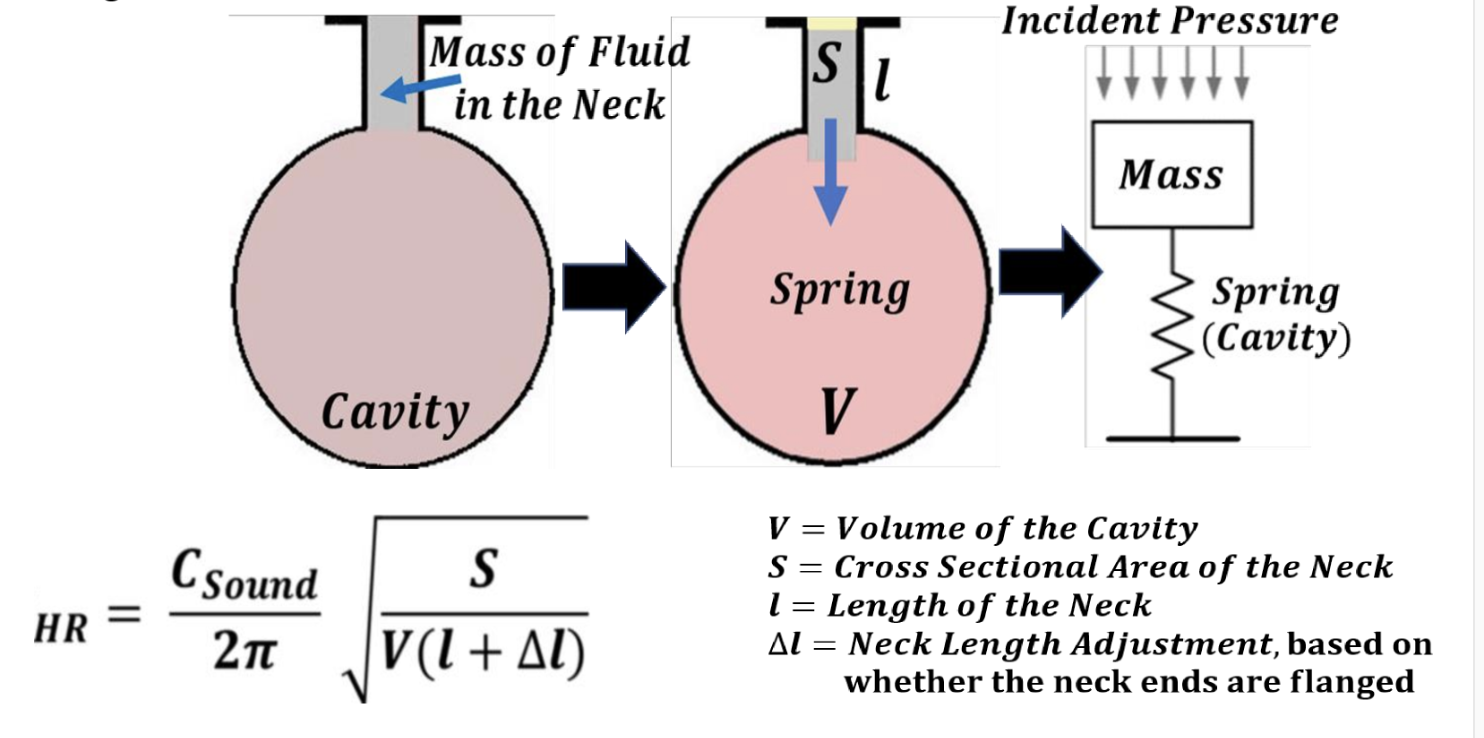
\includegraphics[width=0.8\linewidth,height=\textheight,keepaspectratio]
{images/Hill2018figure2screenshot.png}
\caption{Hill\autocite{Hill2018ResonanceFO} without permission.}\label{fig:resonator}
\end{figure}
We shall return to the question of the analysis of notes at a later stage, after
we have treated of the vibrations of strings, with the aid of which it is best
elucidated; but a very instructive experiment, due originally to Ohm and
improved by Helmholtz, may be given here.  Helmholtz\footnote{Tonempfindungen,
p. 109} took two bottles of the shape represented in the figure, one about
twice as large as the other.  These were blown by streams of air directed
across the mouth and issuing from gutta-percha tubes, whose ends had been
softened and pressed flat, so as to reduce the bore to the form of a narrow
slit, the tubes being in connection with the same bellows. By pouring in water
when the note is too low and by partially obstructing the mouth when the note
is too high, the bottles may be made to give notes with the exact interval of
an octave, such as b and b'. The larger bottle, blown alone, gives a somewhat
muffled sound similar in character to the vowel U; but, when both bottles are
blown, the character of the resulting sound is sharper, resembling rather the
vowel O. For.a short time after the notes had been heard separately Helmholtz
was able to distinguish them in the mixture; but as the memory of their
separate impressions faded, the higher note seemed by degrees to amalgamate
with the lower, which at the same time became louder and acquired a sharper
character. This blending of the two notes may take place even when the high
note is the louder.

Simple tones correspond to simple pendulous vibrations.  27. Seeing now that
notes are usually compound, and that only a particular sort called tones are
incapable of further analysis, we are led to inquire what is the physical
characteristic of tones, to which they owe their peculiarity. What sort of
periodic vibration is it, which produces a simple tone? According to what
mathematical function of the time does the pressure vary in the passage of the
ear? No question in Acoustics can be more important.

The simplest periodic functions with which mathematicians are acquainted are
the circular functions, expressed by a sine or cosine; indeed there are no
others at all approaching them in simplicity. They may be of any period, and
admitting of no other variation (except magnitude), seem well adapted to
produce simple tones. Moreover it has been proved by Fourier, that the most
general single-valued periodic function can be resolved into a series of
circular functions, having periods which are submultiples of that of the given
function. Again, it is a consequence of the general theory of vibration that
the particular type, now suggested as corresponding to a simple tone, is the
only one capable of preserving its integrity among the vicissitudes which it
may have to undergo. Any other kind is liable to a sort of physical analysis,
one part being differently affected from another. If the analysis within the
ear proceeded on a different principle from that effected according to the laws
of dead matter outside the ear, the consequence would be that a sound
originally simple might become compound on its way to the observer. There is no
reason to suppose that anything of this sort actually happens. When it is added
that according to all the ideas we can form on the subject, the analysis within
the ear must take place by means of a physical machinery, subject to the same
laws as prevail outside, it will be seen that a strong case has been made out
for regarding tones as due to vibrations expressed by circular functions. We
are not however left entirely to the guidance of general considerations like
these. In the chapter on the vibration of strings, we shall see that in many
cases theory informs us beforehand of the nature of the vibration executed by a
string, and in particular whether any specified simple vibration is a component
or not. Here we have a decisive test. It is found by experiment that, whenever
according to theory any simple vibration is present, the corresponding tone can
be heard, but, whenever the simple vibration is absent, then the tone cannot be
heard. We are therefore justified in asserting that simple tones and vibrations
of a circular type are indissolubly connected. This law was discovered by Ohm.

\chapter{Harmonic Motions}\label{harmonic-motions} % pdf page 36, LaTeX page 17

28.  Composition of harmonic motions of like period.  The vibrations expressed
by a circular function of the time and variously designated as simple,
pendulous, or harmonic, are so important in Acoustics that we cannot do better
than devote a, chapter to their consideration, before entering on the dynamical
part of our subject. The quantity, whose variation constitutes the vibration,
may be the displacement of a particle measured in a given direction, the
pressure at a fixed point in a fluid medium, and so on.  In any case denoting
it by u, we have
\begin{equation*} u =a \cos(2 \pi t/ \tau ) - \epsilon ), \tag{1}
\end{equation*}
in which a denotes the amplitude, or extreme value of
u; \(\tau\)is the periodic time, or period, after the lapse of which the values
of u recur; and \(\epsilon\) determines the phase of the vibration at the
moment from which t is measured.

Any number of harmonic vibrations of the same period affecting a variable
quantity, compound into another of the same type, whose elements are determined
as follows:
\begin{align*}
u & =\sum a \cos \left(\frac{2 \pi t}{\tau}-\epsilon\right) \\
& =\cos \frac{2 \pi t}{\tau}
\sum \left( a \cos \epsilon+\sin \frac{2 \pi t}{\tau} \Sigma a \sin \epsilon \right) \\
& =r \cos \left(\frac{2 \pi t}{\tau}-\theta\right) \tag{2}.
\end{align*}
if
\begin{equation*} r=\left\{\left(\sum a \cos \epsilon\right)^2+\left(\sum a
\sin \epsilon\right)^2\right\}^{\frac{1}{2}} . \tag{3}
\end{equation*}
and
\begin{equation*} \tan \theta=\frac{ \sum a \sin \epsilon }{\Sigma a \cos
\epsilon} \tag{4}
\end{equation*}
and

For example, let there be two components,
\[
u=a \cos \left(\frac{2 \pi t}{\tau}-\epsilon\right)+
a^{\prime} \cos \left(\frac{2 \pi t}{\tau}-\epsilon^{\prime}\right);
\]
then
\begin{equation*}
r=\left\{a^2+a^{\prime 2}+2 a a^{\prime} \cos
\left(\epsilon-\epsilon^{\prime}\right)\right\}^{\frac{1}{2}} \tag{5}
\end{equation*}
\begin{equation*} \tan \theta= \frac{a \sin \epsilon+a^{\prime}
\sin \epsilon^{\prime}}{a \cos \epsilon+a^{\prime} \cos \epsilon^{\prime}} \tag{6}.
\end{equation*}
Particular cases may be noted. If the phases of the two components agree,
\[u=\left(a+a^{\prime}\right) \cos \left(\frac{2 \pi t}{\tau}-\epsilon\right) .\]

If the phases differ by half a period,
\[u=\left(a-a^{\prime}\right) \cos
\left(\frac{2 \pi t}{\tau}-\epsilon\right),\]
so that if \(a'=a\), \(u\)
vanishes. In this case the vibrations are often said to \textit{interfere}, but
the expression is rather misleading. Two sounds may very properly be said to
interfere, when they together cause silence; but the mere superposition of two
Vibrations (whether rest is the consequence, or not) cannot properly be so
called. At least if this be interference, it is difficult to say what
non-interference can be. It will appear in the course of this work that when
vibrations exceed a certain intensity they no longer compound by mere addition;
\textit{this} mutual action might more properly be called interference, but it
is a phenomenon of a totally different nature from that with which we are now
dealing.

Again, if the phases differ by a quarter or by three-quarters of a period,
\(\cos(\epsilon- \epsilon')=0\), and
\[r= \sqrt{ a^2 +(a')^2}.\]
Harmonic vibrations of given period may be represented by lines drawn from a pole, the
lengths of the lines being proportional to the amplitudes, and the inclinations
to the phases of the vibrations. The resultant of any number of harmonic
vibrations is then represented by the geometrical resultant of the
corresponding lines. For example, if they are disposed symmetrically round the
pole, the resultant of the lines, or vibrations, is zero.
\begin{figure}[htbp]
% pdf page 34 \centering
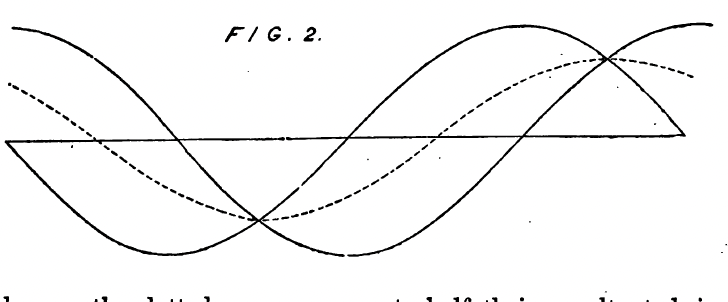
\includegraphics[width=0.8\linewidth,height=\textheight,keepaspectratio]{images/figure2.png}
\caption{Two harmonic curves of the same wave-length and amplitude have
different phases; the dotted curve represents half their resultant, being the
locus of points midway between those in which the two curves are met by any
ordinate.}\label{fig:superposition}
\end{figure}

29.  Harmonic Curve.  If we measure off along an axis of x distances
proportional to the time, and take w for an ordinate, we obtain the harmonic
curve, or curve of sines,
\[ u=a \cos \left(\frac{2 \pi xt}{\lambda}-\epsilon\right), \]
where \(\lambda\), called the wave-length, is
written in place of \(\tau \), both quantities denoting the range of the
independent variable corresponding to a complete recurrence of the function.
The harmonic curve is thus the locus of a point subject at once to a uniform
motion, and to a harmonic vibration in a perpendicular direction. In the next
chapter we shall see that the vibration of a tuning fork is simple harmonic; so
that if an excited tuning fork is moved with uniform velocity parallel to the
line of its handle, a tracing point attached to the end of one of its prongs
describes a harmonic curve, which may be obtained in a permanent form by
allowing the tracing point to bear gently on a piece of smoked paper.


30.  Beats.  If two harmonic vibrations of different periods coexist,
\[
u= a \cos \left(\frac{2 \pi t}{\tau}-\epsilon\right)-
a^{\prime} \cos \left(\frac{2 \pi t}{\tau^{\prime}}-\epsilon^{\prime}\right).
\]
The resultant cannot here
be represented as a simple harmonic motion with other elements.  If \(\tau \)
and \( \tau^{\prime}\) be incommensurable, the value of \(u\) never recurs;
but, if \( \tau \) and \( \tau^{\prime} \) be in the ratio of two whole
numbers, \(u\) recurs after the lapse of a time equal to the east common
multiple of \( \tau \) and \( \tau^{\prime} \); but the vibration is not simple
harmonic.  For example, when a note and its fifth are sounding together, the
vibration recurs after a time equal to twice the period of the graver.

One case of the composition of harmonic vibrations of different periods is
worth special discussion, namely, when the difference of the periods is small.
If we fix our attention on the course of things during an interval of time
including merely a few periods, we see that the two vibrations are nearly the
same as if their periods were absolutely equal, in which case they would, as we
know, be equivalent to another simple harmonic vibration of the same period.
For a few periods then the resultant motion is approximately simple harmonic,
but the same harmonic will not continue to represent it for long. The vibration
having the shorter period continually gains on its fellow, thereby altering the
difference of phase on which the elements of the resultant depend. For
simplicity of statement let us suppose that the two components have equal
amplitudes, frequencies represented by \(m\) and \(n\), where m-n is small, and
that when first observed their phases agree.  At this moment their effects
conspire, and the resultant has an amplitude double of that of the components.
But after a time
\[ \frac{1}{ 2(m-n) } \]
the vibration m will have gained half
a period relatively to the other;.and the two, being now in complete
disagreement, neutralize each other. After a further interval of time equal to
that above named, m will have gained altogether a whole vibration, and complete
accordance is once more re-established. The resultant motion is therefore
approximately simple harmonic, with an amplitude not constant, but varying from
zero to twice that of the components, the frequency of these alterations being
m-n. If two tuning forks with frequencies 500 and 501 be equally excited, there
is every second a rise and fall of sound corresponding to the coincidence or
opposition of their vibrations.

This phenomenon is called beats. We do not here fully discuss the question how
the ear behaves in the presence of vibrations having nearly equal frequencies,
but it is obvious that if the motion in the neighbourhood of the ear almost
ceases for a considerable fraction of a second, the sound must appear to fall.
For reasons that will afterwards appear, beats are best heard when the
interfering sounds are simple tones. Consecutive notes of the stopped diapason
of the organ shew the phenomenon very well, at least in the lower parts of the
scale. A permanent interference of two notes may be obtained by mounting two
stopped organ pipes of similar construction and identical pitch side by side on
the same wind chest. The vibrations of the two pipes adjust themselves to
complete opposition, so that at a little distance nothing can be heard, except
the hissing of the wind. If by a rigid wall between the two pipes one sound
could be cut off, the other would be instantly restored. Or the balance, on
which silence depends, may be upset by connecting, the ear with a tube, whose
other end lies close to the mouth of one of the pipes.

By means of beats two notes may be tuned to unison with great exactness.  The
object is to make the beats as slow as possible, since the number of beats in a
second is equal to the difference of the frequencies of the notes. Under
favourable circumstances beats so slow as one in 30 seconds may be recognised,
and would indicate that the higher note gains only two vibrations a minute on
the lower. Or it might be desired merely to ascertain the difference of the
frequencies of two notes nearly in unison, in which case nothing more is
necessary than to count the number of beats. It will be remembered that the
difference of frequencies does not determine the interval between the two
notes; that depends on the ratio of frequencies. Thus the rapidity of the beats
given by two notes nearly in unison is doubled, when both are taken an exact
octave higher.

% pdf page 40
Analytically
\[u=a \cos (2 \pi m t-\epsilon)+a^{\prime} \cos \left(2 \pi n t-\epsilon^{\prime}\right),\]
where \(m-n\) is small. Now
\(\cos \left(2 \pi n t-\epsilon^{\prime}\right)\)
may be written
\[\cos \left\{2 \pi m t-2 \pi(m-n) t-\epsilon^{\prime}\right\},\]
and we have
\[u=r \cos (2 \pi m t-\theta) \tag{1}, \]
where
\[
r^2=a^2+a^{\prime 2}+2 a a^{\prime} \cos \left\{2 \pi(m-n)
t+\epsilon^{\prime}-\epsilon\right\} \tag{2},
\]
\[
\tan \theta=
\frac{a \sin \epsilon+a^{\prime} \sin \left\{2 \pi(m-n) t+\epsilon^{\prime}\right\}}
{a \cos \epsilon+a^{\prime} \cos \left\{2 \pi(m-n) t+\epsilon^{\prime}\right\}} \tag{3}.
\]
The resultant vibration may thus be considered as harmonic with
elements \(r\) and \(\theta\), which are not constant but slowly varying
functions of the time, having the frequency \(m-n\).  The amplitude \(r\) is at
its maximum when
\[\cos \left\{2 \pi(m-n)
t+\epsilon^{\prime}-\epsilon\right\}=+1,\]
and at its minimum when
\[\cos \left\{2 \pi(m-n) t+\epsilon^{\prime}-\epsilon\right\}=-1,\]
the corresponding
values being \(a+a^{\prime}\) and \(a-a^{\prime}\) respectively.

31.  Fourier's Theorem. Another case of great importance is the composition of
vibrations corresponding to a tone and its harmonics, It is known that the most
general single-valued finite periodic function can be expressed by a series of
simple harmonics
\[ u=a_0+\sum_{n \geq 1} a_n \cos \left(\frac{2 \pi n t}{\tau}-\epsilon_n\right) \tag{1},\]
a theorem usually quoted as Fourier's.
Analytical proofs will be found in Todhunter's \textit{Integral Calculus} and
Thomson and Tait's \textit{Natural Philosophy}; and a line of argument almost
if not quite amounting to a demonstration will be given later in this work. A
few remarks are all that will be required here.

Fourier's theorem is not obvious. A vague notion is not uncommon that the
infinitude of arbitrary constants in the series of necessity endows it with the
capacity of representing an arbitrary periodic function.  That this is an error
will be apparent, when it is observed that the same argument would apply
equally, if one term of the series were omitted; in which case the expansion
would not in general be possible.

Another point worth notice is that simple harmonics are not the only functions,
in a series of which it is possible to expand one arbitrarily given. Instead of
the simple elementary term
\[\cos \left(\frac{2 \pi n t}{\tau}-\epsilon_n\right),\]
we might take
\[
\cos \left(\frac{2 \pi n t}{\tau}-\epsilon_n\right)+
\frac{1}{2} \cos \left(\frac{4 \pi n t}{\tau}-\epsilon_n\right),
\]
formed by adding a similar one in the same phase
of half the amplitude and period. It is evident that these terms would serve as
well as the others; for
\begin{align*}
\cos \left(\frac{2 \pi n t}{\tau}-\epsilon_n\right) &
= \cos \left(\frac{2 \pi n t}{\tau}-\epsilon_n\right)+
  \frac{1}{2} \cos \left(\frac{4 \pi n t}{\tau}-\epsilon_n\right) \\
- & \frac{1}{2}\left\{
       \cos \left(\frac{4\pi nt}{\tau}-\epsilon_n\right)+
  \frac{1}{2} \cos \left(\frac{8\pi nt}{\tau}-\epsilon_n\right)
        \right\} \\
+ & \frac{1}{4}\left\{\cos \left(\frac{8\pi nt}{\tau}-\epsilon_n\right)+
     \frac{1}{2} \cos \left(\frac{16\pi nt}{\tau}-\epsilon_n\right)\right\} \\
- & \ldots \\
\end{align*}
so that each term in Fourier's series,
and therefore the sum of the series, can be expressed by means of the double
elementary terms now suggested. This is mentioned here, because students, not
being acquainted with other expansions, may imagine that simple harmonic
functions are by nature the only ones qualified to be the elements in the
development of a periodic function. The reason of the preeminent importance of
Fourier's series in Acoustics is the mechanical one referred to in the
preceding chapter, and to be explained more fully hereafter, namely, that, in
general, simple harmonic vibrations are the only kind that are propagated
through a vibrating system without suffering decomposition.

32.  Vibrations in perpendicular directions. As in other cases of a similar
character, e.g. Taylor's theorem, if the possibility of the expansion be known,
the coefficients may be determined by a comparatively simple process. We may
write (1) of
\[
u=A_0+\sum_{n\geq 1} A_n \cos \frac{2 n \pi t}{\tau}+
\sum_{n\geq 1} B_n \sin \frac{2 n \pi t}{\tau} \tag{1}.
\]
Multiplying by \(\cos \frac{2 n \pi t}{\tau}\) or
\(\sin \frac{2 n \pi t}{\tau}\), and integrating over a complete period \([0,\tau]\),
we find
\[
\left.\begin{array}{l} A_n=\frac{2}{\tau} \int_0^\tau u \cos \frac{2 n \pi t}{\tau} d t \\
B_n=\frac{2}{\tau} \int_0^\tau u \sin \frac{2 n \pi t}{\tau} d t
\end{array}\right\} \tag{2}
\]
An immediate integration gives
\[A_0=\frac{1}{\tau} \int_0^\tau u d t \tag{3} \]
indicating that \(A_o\) is
the \textit{mean} value of \(u\) throughout the period.

The degree of convergence in the expansion of depends in general on the
continuity of the function and its derivatives. The series formed by successive
differentiations of (1) converge less and less rapidly, but still remain
convergent, and arithmetical representatives of the differential coefficients
of u, so long as these latter are everywhere finite. Thus (Thomson and Tait, \S
77), if all the derivatives up to the m inclusive are free from infinite
values, the series for u is more convergent than one with for coefficients.

\section{Beats of approximate consonances}
32 a.  The general explanation of the beats beard when two pure tones nearly in
union are sounded simultaneously has been discussed in § 80. But the occurrence
of beats is not confined to the case of approximate unison, at least when we
have to deal with compound notes. Suppose for example that the interval is an
octave. The graver note then usually includes a tone coincident in pitch with
the fundamental tone of the higher note.

If the interval be disturbed, the previously coincident tones separate
from one another, and give rise to beats of the same frequency as if
they existed alone. There is usually no difficulty in observing these
beats; but if one or both of the component tones concerned be very
faint, the aid of a resonator may be invoked.

In general we may consider that each consonant interval is characterized
by the coincidence of certain component tones, and if the interval be
disturbed the previously coincident tones give rise to beats. Of course
it may happen in any particular case that the tones which would coincide in
pitch are absent from one or other of the notes. The disturbance of the
interval would then, according to the above theory, not be attended by beats.
In practice faint beats are usually heard; but the discussion of this
phenomenon, as to which authorities are not entirely agreed, must be postponed.

33. Consonant intervals. Another class of compounded vibrations, interesting
from the facility with which they lend themselves to optical observation, occur
when two harmonic vibrations affecting the same particle are executed in
perpendicular directions, more especially when the periods are not only
commensurable, but in the ratio of two small whole numbers. The motion is then
completely periodic, with a period not many times greater than those of the
components, and the curve described is re-entrant. If w and v be the
coordinates, we may take
\[u=a \cos(2rnt-\epsilon), \quad v=b \cos(Qrm t) (1).\]
First let us suppose that the periods are equal, so that n'=n; the elimination
of t ges for the equation of the curve described,
\[\frac{u^2}{a^2}+\frac{v^2}{b^2}-\frac{2uv}{ab}\cos(\epsilon)-\sin^2(\epsilon)=0,\]
(2) representing in general an ellipse, whose position and dimensions depend
upon the amplitudes of the original vibrations and upon the difference of their
phases. If the phases differ by a quarter period, \(\cos(e)=0\), and the equation becomes
\[ \frac{u^2}{a^2} +  \frac{v^2}{b^2} =1.  \]

In this case the axes of the ellipse coincide with those of coordinates, If
further the two components have equal amplitudes, the locus degenerates into
the circle
\[ u^2 +  v^2 = a^2,\]
which is described with uniform velocity.
This shews how a uniform circular motion may be analysed into two rectilinear
harmonic motions, whose directions are perpendicular.

If the phases of the components agree, \(\epsilon = 0\), and the ellipse
degenerates into the coincident straight lines
\[ \left( \frac{u}{a} - \frac{v}{b}\right)^2 = 0 \]
if the difference of phase amount to half a period,
\[ \left( \frac{u}{a} + \frac{v}{b}\right)^2 = 0 \]

When the unison of the two vibrations is exact, the elliptic path remains
perfectly steady, but in practice it will almost always happen that there is a
slight difference between the periods. The consequence is that though a fixed
ellipse represents the curve described with sufficient accuracy for a few
periods, the ellipse itself gradually changes in correspondence with the
alteration in the magnitude of . It becomes therefore a matter of interest to
consider the system of ellipses represented by (2), supposing a and b
constants, but e variable.

Since the extreme values of u and v are +a, +b respectively, the ellipse is in
all cases inscribed in the rectangle whose sides' are 2a, 2b.  Starting with
the phases in agreement, or e=0, we have the ellipse coincident with the
diagonal F =0. As e increases from 0 to 7, the ellipse opens out until its equation becomes

From this point it closes up again, ultimately coinciding with the other
diagonal - + = 0, corresponding to the increase of e from 3a to m.  After this,
as e ranges from a to 27, the ellipse retraces its course until it again
coincides with the first diagonal. The sequence of changes is exhibited in Fig.  3,

FIG.3.

The ellipse, having already four given tangents, is completely determined by
its point of contact P (Fig. 4) with the line v=d.

In order to connect this with \(\epsilon\), e, it is sufficient to observe that
when \(v=b\), \(\cos(2 \pi nt) =1\); and therefore \(u=a \cos(\epsilon)\). Now
if the elliptic paths be the result of the superposition of two harmonic
vibrations of nearly coincident pitch, \(\epsilon\) varies uniformly with the
time, so that P itself executes a harmonic vibration along AA' with a frequency
equal to the difference of the two given frequencies.

34.  Lissajous’ Cylinder. Lissajous\footnote{Annales de Chimie (3) LI  147}
has shewn that this system of ellipses may be regarded as the different aspects
of one and the same ellipse described on the surface of a transparent cylinder.
In Fig. 5 A A' B' B represents the cylinder, of which AB' is a plane section.
Seen from an infinite distance in the direction of the common tangent at A to
the plane sections, the cylinder is projected into a rectangle, and the ellipse
into its diagonal. Suppose now that the cylinder turns upon its axis, carrying
the plane section with it. Its own projection remains a constant rectangle in
which the projection of the ellipse is inscribed. Fig. 6 represents the
position of the cylinder after a rotation through a right angle. It appears
therefore that by turning the cylinder round we obtain in succession all the
ellipses corresponding to the paths described by a point subject to two
harmonic vibrations of equal period and fixed amplitudes. Moreover if the
cylinder be turned continuously with uniform velocity, which insures a harmonic
motion for P, we obtain a complete representation of the varying orbit
described by the point when the periods of the two components differ slightly,
each complete revolution answering to a gain or loss of a single vibration
\footnote{By a vibration will always be meant in this work a complete cycle of
changes}. The revolutions of the cylinder are thus synchronous with the beats
which would result from the composition of the two vibrations, if they were to
act in the same direction.

FIG. 5.  FIG. 6.

35. Lissajous' Figures. Vibrations of the kind here considered are very easily
realized experimentally. A heavy pendulum-bob, hung from a fixed point by a
long wire or string, describes ellipses under the action of gravity, which may
in particular cases, according to the circumstances of projection, pass into
straight lines or circles. But in order to see the orbits to the best
advantage, it is necessary that they should be described so quickly that the
impression on the retina made by the moving point at any part of its course has
not time to fade materially, before the point comes round again to renew its
action. This condition is fulfilled by the vibration of a silvered bead (giving
by reflection a luminous point), which is attached to a straight metallic wire
(such as a knitting-needle), firmly clamped in a vice at the lower end.  When
the system is set into vibration, the luminous point describes ellipses, which
appear as fine lines of light. These ellipses would gradually contract in
dimensions under the influence of friction until they subsided into a
stationary bright point, without undergoing any other change, were it not that
in all probability, owing to some want of symmetry, the wire has slightly
differing periods according to the plane in which the vibration is executed.
Under these circumstances the orbit is seen to undergo the cycle of changes
already explained.

36. Optical methods of composition and analysis. So far we have supposed the
periods of the component vibrations to be equal, or nearly equal; the next case
in order of simplicity is when one is the double of the other. We have
\[u=a \cos(4n \pi t-\epsilon), \quad v= b \cos(2n \pi t).\]
The locus resulting from the elimination of \(t\) may be written
\[
\frac{u}{a} = \left( 2 \frac{v^2}{b^2} -1 \right) \cos (\epsilon ) +
\frac{2v}{b} \sqrt{1-\frac{v^2}{b^2}} ~~ \sin(\epsilon),
\]
(1) which for all values of \(\epsilon\) represents a curve inscribed in the
rectangle 2a, 2b.  \todo[inline]{ exponent of 2nd v smudged in text} If e=0, or
7, we have

o u 2 - a) (1 + i), representing parabolas, Fig. 7 shews the various curves for
the intervals of the octave, twelfth, and fifth.

\todo[inline]{Z is a sigma for summation} FIG C Z

To all these systems Lissajous' method of representation by the transparent
cylinder is applicable, and when the relative phase is altered, whether from
the different circumstances of projection in different cases, or continuously
owing to a slight deviation from exactness in the ratio of the periods, the
cylinder will appear to turn, so as to present to the eye different aspects of
the same line traced on its surface.

37.  Blackburn's pendulum.  There is no difficulty in arranging a vibrating
system so that the motion of a point shall consist of two harmonic vibrations
in perpendicular planes, with their periods in any assigned ratio, The simplest
is that known as Blackburn's pendulum. A wire ACB is fastened at A and B, two
fixed points at the same level, The bob P is attached to its middle point by
another wire CP. For vibrations in the plane of the diagram, the point of
suspension is practically C, provided that the wires are sufficiently
stretched; but for a motion perpendicular to this plane, the bob turns about D,
carrying the wire 4 OB with it. The periods of vibration in

A; 0 : B

the principal planes are in the ratio of the square roots of CP and DP.  Thus
if DC=3CP, the bob describes the figures of: the octave. To obtain the sequence
of curves corresponding to approximate unison ACB must be so nearly tight, that
CD is relatively small.

38.  Kaleidophone.  Another contrivance called the kaleidophone was originally
invented by Wheatstone. A straight thin bar of steel carrying a bead at its
upper end is fastened in a vice, as explained in a previous paragraph. If the
section of the bar is square, or circular, the period of vibration is
independent of the plane in which it is performed. But let us suppose that the
section is a rectangle with unequal sides. The stiffness of the bar --the force
with which it resists bending-- is then greater in the plane of greater
thickness, and the vibrations in this plane have the shorter period.  By a
suitable adjustment of the thicknesses, the two periods of vibration may be
brought into any required ratio, and the corresponding curve exhibited.

The defect in this arrangement is that the same bar will give only one set of
figures. In order to overcome this objection the following modification has
been devised. A slip of steel is taken whose rectangular section is very
elongated, so that as regards bending in one plane the stiffness is so great as
to amount practically to rigidity.  The bar is divided into two parts, and the
broken ends reunited, the two pieces being turned on one another through a
right angle, so that the plane, which contains the small thickness of one,
contains the great thickness of the ether. When the compound rod is clamped in
a vice at a point below the junction, the period of the vibration in one
direction, depending almost entirely on the length of the upper piece, is
nearly constant; but that in the second direction may be controlled by varying
the point at which the lower piece is clamped.

39. In this arrangement the luminous point itself executes the vibrations which
are to be observed; but in Lissajous' form of the experiment, the point of
light remains really fixed, while its image is thrown into apparent motion by
means of successive reflection from two vibrating mirrors. A small hole in an
opaque screen placed close to the flame of a lamp gives a point of light, which
is observed after reflection in the mirrors by means of a small telescope. The
mirrors, usually of polished steel, are attached to the prongs of stout tuning
forks, and the whole is so disposed that when the forks are thrown into
vibration the luminous point appears to describe harmonic motions in
perpendicular directions, owing to the angular motions of the reflecting
surfaces. The amplitudes and periods of these harmonic motions depend upon
those of the corresponding forks, and may be made such as to give with enhanced
brilliancy any of the figures possible with the kaleidophone. By a similar
arrangement it is possible to project the figures on a screen. In either case
they gradually contract as the vibrations of the forks die away.

40. The principles of this chapter have received an important application in
the investigation of rectilinear periodic motions. When a point, for instance a
particle of a sounding string, is vibrating with such a period as to give a
note within the limits of hearing, its motion is much too rapid to be followed
by the eye; so that, if it be required to know the character of the vibration,
some indirect method must be adopted. The simplest, theoretically, is to
compound the vibration under examination with a uniform motion of translation
in a perpendicular direction, as when a tuning fork draws a harmonic curve on
smoked paper.  Instead of moving the vibrating body itself, we may make use of
a revolving mirror, which provides us with an image in motion. In this way we
obtain a representation of the function characteristic of the vibration, with
the abscissa proportional to time.

But it often happens that the application of this method would be difficult or
inconvenient. In such cases we may substitute for the uniform motion a harmonic
vibration of suitable period in the same direction. To fix our ideas, let us
suppose that the point, whose motion we wish to investigate, vibrates
vertically with a period 7, and let us examine the result of combining with
this a horizontal harmonic motion, whose period is some multiple of 1, say, nr.
Take a rectangular piece of paper, and with axes parallel to its edges draw the
curve representing the vertical motion (by setting off abscissa proportional to
the time) on such a scale that the paper just contains repetitions or waves,
and then bend the paper round so as to form a cylinder, with a re-entrant curve
running round it. A point describing this curve in such a manner that it
revolves uniformly about the axis of the cylinder will appear from a distance
to combine the given vertical motion of period 7, with a horizontal harmonic
motion of period nr. Conversely therefore, in order to obtain the
representative curve of the vertical vibrations, the cylinder containing the
apparent path must be imagined to be divided along a generating line, and
developed into a plane. There is less difficulty in conceiving the cylinder and
the situation of the curve upon it, when the adjustment of the periods is not
quite exact, for then the cylinder appears to turn, and the contrary motions
serve to distinguish those parts of the curve which lie on its nearer and
further face.

41. The vibration microscope.  The auxiliary harmonic motion is generally
obtained optically, by means of an instrument called a vibration-microscope
invented by Lissajous. One prong of a large tuning fork carries a lens, whose
axis is perpendicular to the direction of vibration; and which may be used
either by itself, or as the object-glass of a compound microscope formed by the
addition of an eye-piece independently supported. In either case a stationary
point is thrown into apparent harmonic motion along a line parallel to that of
the fork's vibration.

The vibration-microscope may be applied to test the rigour and universality of
the law connecting pitch and period. Thus it will be found that any point of a
vibrating body which gives a pure musical note will appear to describe a
re-entrant curve, when examined with a vibration-microscope whose note is in
strict unison with its own. By the same means the ratios of frequencies
characteristic of the consonant intervals may be verified; though for this
latter purpose a more thoroughly acoustical method, to be described in a future
chapter, may be preferred.

42. Intermittent illumination.  Another method of examining the motion of a
vibrating body depends upon the use of intermittent illumination
\footnote{Plateau, Bull. de l'Aca. roy. de Belgique, t. III, p. 364, 1836}.
Suppose, for example, that by means of suitable apparatus a series of electric
sparks are obtained at regular intervals \(\tau\).  A vibrating body, whose
period is also \(\tau\), examined by the light of the sparks must appear at
rest, because it can be seen only in one position. If, however, the period of
the vibration differ from \(\tau\) ever so little, the illuminated position
varies, and the body will appear to vibrate slowly with a frequency which is
the difference of that of the spark and that of the body. The type of vibration
can then be observed with facility.

The series of sparks can be obtained from an induction-coil, whose primary
circuit is periodically broken by a vibrating fork, or by some other
interrupter of sufficient regularity. But a better result is afforded by
sunlight rendered intermittent with the aid of a fork, whose prongs carry two
small plates of metal, parallel to the plane of vibration and close together.
In each plate is a slit parallel to the prongs of the fork, and so placed as to
afford a free passage through the plates when the fork is at rest, or passing
through the middle point of its vibrations. On the opening so formed, a beam of
sunlight is concentrated by means of a burning glass, and the object under
examination is placed in the cone of rays diverging on the further side
\footnote{Topler, Phil. Mag. Jan. 1867.}.  When the fork is made to vibrate by
an electromagnetic arrangement, the illumination is cut off except when the
fork is passing through its position of equilibrium, or nearly so. The flashes
of light obtained by this method are not so instantaneous as electric sparks
(especially when a jar is connected with the secondary wire of the coil), but
in my experience the regularity is more perfect. Care should be taken to cut
off extraneous light as far as possible, and the effect is then very striking.

A similar result may be arrived at by looking at the vibrating body through a
series of holes arranged in a circle on a revolving disc.  Several series of
holes may be provided on the same disc, but the observation is not satisfactory
without some provision for securing uniform rotation.

Except with respect to the sharpness of definition, the result is the same when
the period of the light is any multiple of that of the vibrating body. This
point must be attended to when the revolving wheel is used to determine an
unknown frequency.

When the frequency of intermittence is an exact multiple of that of the
vibration, the object is seen without apparent motion, but generally in more
than one position. This condition of things is sometimes advantageous.

Similar effects arise when the frequencies of the vibrations and of the flashes
are in the ratio of two small whole numbers. If, for example, the number of
vibrations in a given time be half as great again as the number of flashes, the
body will appear stationary, and in general double.

\section{Random phases.}
42 a.  We have seen (§ 28) that the resultant of two isoperiodic vibrations of equal
amplitude is wholly dependent upon their phase relation, and it is of interest
to inquire what we are to expect from the composition of a large number \(n\)
of equal vibrations of amplitude unity, of the same period, and of phases
accidentally determined. The intensity of the resultant, represented by the
square of the amplitude § 245, \todo[inline]{volume 2 article245?} will of
course depend upon the precise manner in "which the phases are distributed, and
may vary from \(n^2\) to zero. But is there a definite intensity which becomes
more and more probable when \(n\) is increased without limit?

The nature of the question here raised is well illustrated by the special case
in which the possible phases are restricted to two opposite phases. We may then
conveniently discard the idea of phase, and regard the amplitudes as at random
positive or negative. If all the signs be the same, the intensity is \(n^2\);
if, on the other hand, there be as many positive as negative, the result is
zero. But although the intensity may range from 0 to \(n^2\), the smaller
values are more probable than the greater.

The simplest part of the problem relates to what is called in the theory of
probabilities the \textit{expectation} of intensity, that is, the mean
intensity to be expected after a great number of trials, in each of which the
phases are taken at random. The chance that all the vibrations are positive is
\(2^{-n}\) and thus the expectation of intensity corresponding to this
contingency is \(2^{-n} n^2\).  In like manner the expectation corresponding to
the number of positive vibrations being \(n-1\) is
\[2^{-n} n (n-2)^2,\]
and so on. The whole expectation of intensity is thus
\[
2^{-n} \left( \begin{pmatrix} n \\ 0 \end{pmatrix} n^2 +
\begin{pmatrix} n \\ 1\\ \end{pmatrix} (n-2)^2 +
\begin{pmatrix} n \\ 2\\ \end{pmatrix} (n-4)^2 + \ldots \right) =
\]
\[ 2^{-n} \sum_{k=0}^n \begin{pmatrix} n \\ k \end{pmatrix} (n-2k)^2. \]
(1) Now the sum of the (n + 1) terms of this series is simply \(n\), as may be
proved by comparison of coefficients of \(x^2\) in the equivalent forms

The expectation of intensity is therefore \(n\), and this whether \(n\), be great or small.

The same conclusion holds good when the phases are unrestricted. From (3) § 28,
if \(a_1 = a_2 = \ldots = 1\),
\[
r^2 = (cos \epsilon_1 + cos \epsilon_2 + \ldots)^2 +
      (sin \epsilon_1 + sin \epsilon_2 + \ldots)^2
\]
\[ n + 2 \sum cos ( \epsilon_2 - \epsilon_1 ) \]
(2), where under the sign of summation are to be included the cosines
of the \(n(n-1)/2\) differences of phase. When the phases are
accidentally the sum is as likely to be positive as negative;
and thus the mean value of
\(r^2\)
is
\(n\).

The reader must be on his guard here against a fallacy, which has misled
some eminent authors. We have nut proved that when n is large there is
any tendency for a single combination to give an intensity equal to n,
but the quite different proposition that in a large number of trials, in
e h of which the phases are distributed at random, the mean intensity
will tend more and more to the value n. It is true that even in a single
combination there is no reason why any of the cosines in (2) should be
positive rather than negative. From this we may infer that when n is
increased the sum of the terms tends to vanish in comparison with the number of
terms; but, the number of the terms being of the order n we can infer nothing
as to the value of the sum of the series in comparison with n.

So far there is no difficulty; but a complete investigation of this
subject involves an estimate of the relative probabilities of resultants
lying within assigned limits of magnitude. For example, we ought to be
able to say what is the probability that the intensity due to a large
number (re) of equal components is less than n. This problem may
conveniently be considered here, though it is naturally beyond the reach
of elementary methods. We will commence by taking it under the
restriction that the phases are of two opposite kinds only.

Adopting the statistical method of statement, let us suppose that there
are an immense number N of independent combinations, each consisting of
n unit vibrations, positive or negative, and combined accidentally. When
N is sufficiently large, the statistics become regular; and the number
of combinations in which the resultant amplitude is found equal to x may
be denoted by
\( N f(n, x)\), where
\(f\) is a definite function of
\(n\) and \(x\). Now suppose that each of the N
combinations receives another random contribution of ± 1, and inquire
how many of them will subsequently possess a resultant x. It is clear
that those only can do so which originally had amplitudes x-1 or x+1.
Half of the former, and half of the latter number will acquire the
amplitude x,
so that the number required is
\[ \frac{1}{2} Nf(n, x-1) + \frac{1}{2} Nf(n,x+1).\]
But this must be identical with the number corresponding to
\(n + 1\) and \(x\), so that
\[f(n+1, x)=\frac{1}{2} f(n,x-1) + \frac{1}{2} f(n,x+1).\]
(3) This equation of differences holds good for all integral values of a and
for all positive integral values of n. If f(n, a) he given for one value
of n, the equation suffices to determine (n, x) for all higher integral
values of n. For the present purpose the initial value of a is zero. In
that case we know that for
all values of x other than zero, and that when x = 0,(0, 0) = 1.

The problem proposed in the above form is perfectly definite ; but for
our immediate object it suffices to limit ourselves to the supposition
that n is great, regarding (a, d) as a continuous function of continuous
variables n and x, much as in the analogous problem of §§ 120, 121, 122.

Writing (3) in the form
\[f(n+1,x)-f(n,x)=\frac{1}{2} f(n,x-1) + \frac{1}{2} f(n,x+1) -f(n,x),\]
(4) we see that the left-hand member may then be identified with
\( df/dn\), and
the right-hand member with
\todo[inline]{I am not typing the correct equation}
\( df/dn\),
so that under
these circumstances the differential equation to which (3) reduces is of
the well-known form
\[ df/dn = df/dn.\]
(5)

The analogy with the conduction of heat is indeed very close; and the methods
developed by Fourier for the solution of problems in the latter subject are at
once applicable. The special condition here is that initially, that is when \(n
= 0\), \(f\) must vanish for all values of x other than zero. As may be
verified by differentiation, the special solution of (5) is then

(6)
in which is an \(A\) is an arbitrary constant to he determined from the
consideration that the whole number of combinations is \(N\).  Thus if \(dx\)
be large in comparison with unity, the number of combinations which have
amplitudes between \(x\) and \(x + dx\) is

while

so that in virtue of the known equality

\[ A \sqrt{2 \pi} = 1.\]

The final result for the number of combinations which have amplitudes between
\(x\) and \(x + dx\) is accordingly

The mean intensity is expressed by

as before.

We will now pass on to the more important problem in which the phases of
the n unit vibrations are distributed at random over the entire period.
In each combination the resultant amplitude is denoted by \(r\) and the
phase (referred to a given epoch) by
\(\theta \)
; and rectangular coordinates are taken so that
\[ x =r \cos \theta, y =r \sin \theta.\]
Thus any point (x, y) in the plane of reference represents a vibration
of amplitude \(r\) and phase
\(\theta \)
, and the whole system of
\(N\)
vibrations is
represented by a distribution of points, whose density it is our object
to determine. Since no particular phase can be singled out for
distinction, we know beforehand that the density of distribution will be
independent of \(\theta \).

Of the infinite number N of points we suppose that
\[
Nf n, X, y) dxdy
\]
are to be found within the infinitesimal area dxdy, and we will inquire as
before how this number would be changed by the addition to the n
component vibrations of one more unit vibration of accidental phase. Any
vibration which after the addition is represented by the point x, y must
before have corresponded to the point
\[ x' = x \cos \phi, y' = y' - \sin \phi.\]
where
\(\phi \)
represents the phase of the additional unit vibration. And, if for the
moment be regarded as given, to the area dxdy corresponds an equal area
\( dx' dy' \). Again, all values of
\(\phi \)
being equally probable, the factor necessary
under this head is
\(d \phi/(2 \pi) \).
Accordingly the whole number to be found in dx dy
after the superposition of the additional unit is

Ndxdy;

and this is to be equated to

Ndxdyf(n + 1, x, y);

so  that
f(n + 1, x, y) = (8).

The value of f (n, x', y') is
obtained by introduction of the values of x', y' and expansion:

( '. y') (
. y) - + 5 cos sin + 5 y sin B +

so that

( y') 2ir = ( y) + i

Also, n being very great,

f(n + 1, x, y) -f (n, x, y) = df/dn ;

and (8) reduces to
(9)
the usual equation for the conduction of heat in two dimensions.

In addition to (9), f has to satisfy the special condition of evanescence
when n 0 for all points other than the origin. The appropriate solution
is necessarily symmetrical round the origin, and takes the form (n, X,
y) = (10),

as may be verified by differentiation. The constant A is to
be determined by the condition that the whole number is N, Thus N = NArr
j dxdy NA 27ri J e rdr irAN

and the number of vibrations within the
area dxdy becomes e-w+ rfar(iM (11). ini

If we wish to find the number of vibrations which have amplitudes between \(r\) and
\(r+dr\),
 we must introduce polar coordinates and integrate with respect to
0.
The required number is thus \footnote{Phil. Mag. Aug. 1880.} (12)

The result may also be expressed by saying that the probability
of a resultant amplitude between \(r\) and \(r+dr\) when a large
number n of unit vibrations are compounded at random is

rr e- i rdr (13).

The mean intensity is given by 2n''\,' I = Jo as was to be expected. The
probability of a resultant amplitude less than \(r\) is J er rdr = 1 - (14),
or, which is the same thing, the probability of a resultant amplitude
greater than \(r\) is (15). The following table gives the probabilities of
intensities less than the fractions of n named in the first column. For
example, the probability of intensity less than n is 6321.
\begin{table}[h]
\centering
\begin{tabular}{cccc}
0.05 & 0.0488 & 0.80 & 0.5506\\
0.10 & 0.0952 & 100 & 0.6321\\
0.20 & 0.1813 & 1.50 & 0.7768\\
0.40 & 0.3296 & 2.00 & 0.8647\\
0.60 & 0.4512 & 3.00 & 0.9502\\
\end{tabular}
\caption{something tablulated on [0,3].}
\end{table}
It will be seen that, however great \(n\) may be, there is a reasonable, chance
of considerable relative fluctuations of intensity in different combinations.

If the amplitude of each component be a, instead of unity, as we have
hitherto supposed for brevity, the probability of a resultant amplitude
between \(r\) and \(r+dr\) is

e~ l 'rdr (16). The result is thus a function of n and a only through na
and would be unchanged if for example the amplitude became ti and the
number 4n. From this it follows that the law is not altered, even if the
components have different amplitudes, provided always that the whole
number of each kind is very great; so that if there be n components of
amplitude a, n of amplitude 9, and so on, the probability of a resultant
between \(r\) and r H-rfr is wa + n fP + That this is the case may perhaps
be made more clear by the consideration of a particular case. Let us
suppose in the first place that n+47i unit vibrations are compounded at random.

The appropriate law is given at once by (13) on substitution of n + 4n'
for that is

2 (n + rdr (18)i ` Now the combination of n+4n' unit vibrations may be
regarded as arrived at by combining a random combination of n unit
vibrations with a second random combination of 4n' units, and the second
random combination is the same as if due to a random combination of n'
vibrations each of amplitude 2 Thus (18) applies equally well to a
random combination of (n + n') vibrations, n of which are of amplitude
unity and a' of amplitude 2.

Although the result has no application to the theory of vibrations, it
may be worth notice that a similar method applies to the composition tn
three dimensions of unit vectors, whose directions are accidental. The
equation analogous to (8) gives in place of (9)

dn 6Vd dy ds

The appropriate solution, analogous to (13), is

V(is) ( )
expressing the probability of a resultant amplitude lying between \(r\) and
\(r+dr\) expressing the probability of a resultant amplitude lying
between \(r\) and \(r+dr\).

Here again the mean value of \(r^2\), to be expected in a great
number of independent combinations, is \(n\).

\chapter{Systems Having One Degree of Freedom}
\label{systems-having-one-degree-of-freedom}

43. The material systems, with whose vibrations Acoustics is concerned, are
usually of considerable complication, and are susceptible of very various modes
of vibration, any or all of which may coexist at any particular moment. Indeed
in some of the most important musical instruments, as strings and organ-pipes,
the number of independent modes is theoretically infinite, and the
consideration of several of them is essential to the most practical questions
relating to the nature of the consonant chords. Cases, however, often present
themselves, in which one mode is of paramount importance; and even if this were
not so, it would still be proper to commence the consideration of the general
problem with the simplest case-that of one degree of freedom. It need not be
supposed that the mode treated of is the only one possible, because so long as
vibrations of other modes do not occur their possibility under other
circumstances is of no moment.

\setcounter{equation}{0}

44.  Independence of amplitude and period.
The condition of a system possessing one degree of freedom is defined by
the value of a single coordinate u, whose origin may be taken to correspond to
the position of equilibrium. The kinetic and potential energies of the system
for any given position are proportional respectively to
\(\dot{u}^2\)
and
\(u^2\):
\begin{equation}
T= \frac{1}{2} m \dot{u}^2, \quad V = \frac{1}{2} \mu u^2
\end{equation}
where \(m\) and \(\mu\) are in general functions of \(u\). But if we
limit ourselves to the consideration of positions in the immediate
neighbourhood of that corresponding to equilibrium,
\(u\) is a small quantity, and
\(m\) and \(\mu\)
are sensibly constant. On this understanding we now proceed. If there be
no forces, either resulting from internal friction or viscosity, or impressed
on the system from without, the whole energy remains constant. Thus
\[
T+V=\textrm{constant}.
\]

Substituting for
\(T\) and \(V\)
their values, and differentiating with respect to the
time, we obtain the equation of motion
\begin{equation}
m \ddot{u} + \mu u = 0;
\end{equation}

of which the complete integral is
\begin{equation}
u = a \cos( nt - \alpha )
\end{equation}
where \(n^2 = \mu/m\), representing a harmonic vibration. It
will be seen that the period alone is determined by the nature of the system
itself; the amplitude and phase depend on collateral circumstances, If the
differential equation were exact, that is to say, if
\(T \propto \dot{u}^2\),
 and
\(V \propto u^2\), then, without any restriction, the
vibrations of the system about its configuration of equilibrium would be
accurately harmonic, But in the majority of cases the proportionality is only
approximate, depending on an assumption that the displacement
\(u\)
is always small
-- how small depends on the nature of: the particular system and the degree of
approximation required; and then of course we must be careful not to push the
application of the integral beyond its proper

But, although not to be stated without a limitation, the principle that the
vibrations of a system about a configuration of equilibrium have a period
depending on the structure of the system and not on the particular
circumstances of the vibration, is of supreme importance, whether regarded from
the theoretical or the practical side. If the pitch and the loudness of the
note given by a musical instrument were not within wide limits independent, the
art of the performer on many instruments, such as the violin and pianoforte,
would be revolutionized,

The periodic time
\begin{equation}
\tau = \frac{2 \pi}{n} = 2 \pi \frac{m}{\mu}
\end{equation}
\(m\) and \(\mu\)
so that an increase in
\(m\), or a decrease in
\(\mu\), protracts the duration of a
vibration. By a generalization of the language employed in the case of a
material particle urged towards a position of equilibrium by a spring,
\(m\)
may be
called the inertia of the system, and
\(\mu\) the force of the equivalent spring.
Thus an augmentation of mass, or a relaxation of spring, increases the periodic
time. By means of this principle we may sometimes obtain limits for the value
of a period, which cannot, or cannot easily, be calculated exactly.

45. Dissipative Forces.  The absence of all forces of a frictional character is
an ideal case, never realized but only approximated to in practice. The
original energy of a vibration is always dissipated sooner or later by
conversion into heat. But there is another source of loss, which though not,
properly speaking, dissipative, yet produces results of much the same nature.
Consider the case of a tuning fork vibrating \textit{in vacuo}. The internal
friction will in time stop the motion, and the original energy will be
transformed into heat. But now suppose that the fork is transferred to an open
space. In strictness the fork and the air surrounding it constitute a single
system, whose parts cannot be treated separately. In attempting, however, the
exact solution of so complicated a problem, we should generally be stopped by
mathematical difficulties, and in any case an approximate solution would be
desirable. The effect of the air during a few periods is quite insignificant,
and becomes important only by accumulation. We are thus led to consider its
effect as a disturbance of the motion which would take place \textit{in vacuo}.
The disturbing force is periodic (to the same approximation that the vibrations
are so), and may be divided into two parts, one proportional to the
acceleration, and the other to the velocity. The former produces the same
effect as an alteration in the mass of the fork, and we have nothing more to do
with it at present. The latter is a force arithmetically proportional to the
velocity, and always acts in opposition to the motion, and therefore produces
effects of the same character as those due to friction. In many similar cases
the loss of motion by communication may be treated under the same head as that
due to dissipation proper, and is represented in the differential equation with
a degree of approximation sufficient for acoustical purposes by a term
proportional to the velocity. Thus
\begin{equation}
\ddot{u} + \kappa \dot{u} + n^2 u = 0;
\end{equation}
is the equation of vibration for a
system with one degree of freedom subject to frictional forces. The solution is
\begin{equation}
u=A e^{-\kappa t/2}\cos \left(t \sqrt{n^2 - \kappa^2/4} -\alpha \right).
\end{equation}

If the friction be so great that \(\kappa^2/4 > n^2\),
the solution changes its form, and no longer corresponds to an oscillatory
motion; but in all acoustical applications
\(\kappa\)
is a small quantity. Under these
circumstances (2) may be regarded as expressing a harmonic vibration, whose
amplitude is not constant, but diminishes in geometrical progression, when
considered after equal intervals of time. The difference of the logarithms of
successive extreme excursions is nearly constant, and is called the Logarithmic
Decrement. It is expressed by
\(\kappa \tau/4\), if
\(\tau \)
be the periodic time.

The frequency, depending on
\( n^2 - \kappa^2/4 \), involves only the second power of ; so that
to the first order of approximation the friction has no effect on the period,-a
principle of very general application.

The vibration here considered is called the free vibration. It is that executed
by the system, when disturbed from equilibrium, and then left to itself.

46. Forced Vibrations.  We must now turn our attention to another problem, not
less important, the behaviour of the system, when subjected to a force varying
as a harmonic function of the time. In order to save repetition, we may take at
once the more general case including friction. If there be no friction, we have
only to put in our results x=0. The differential equation is

\[t + K + \nu = E \cos(pl) (1).\]

Assume \(U =A \cos(Pt -E) (2),\) and substitute :

\[a (n  - p ) \cos(pt-e) - pa \sin(pt)- e) = E \cos(c \cos(pt-e) - H \sin(e) \sin(pt-e); \]
whence, on equating coefficients of \(\cos(pt-c),\)
\(\sin(pt-),\)
\[a(n - p ) = E \cos(e) a p= E \sin(e)\]
so that the solution
may be written \(\sin(re) C (pt) ++\) (4), where \(\tan(c), (D)e\).

This is called a forced vibration; it is the response of the system to a force
imposed upon it from without, and is maintained by the continued operation of
that force. The amplitude is proportional to Z --the magnitude of the force,
and the period is the same as that of the force.

Let us now suppose Z given, and trace the effect on a given system of a
variation in the period of the force. The effects produced in different cases
are not strictly similar; because the frequency of the vibrations produced is
always the same as that of the force, and therefore variable in the comparison
which we are about to institute. We may, however, compare the energy of the
system in different cases at the moment of passing through the position of
equilibrium. It is necessary thus to specify the moment at which the energy is
to be computed in each case, because the total energy is not invariable
throughout the vibration.  During one part of the period the system receives
energy from the impressed force, and during the remainder of the period yields
it back again.

From (4), if u=0,

energy \(w w \sin(e)\) and is therefore a maximum, when sine=1, or, from (5),
p=n. If the maximum kinetic energy be denoted by 7, we have

THT, Sin7 (6).

The kinetic energy of the motion is therefore the greatest possible, when the
period of the force is that in which the system would vibrate freely under the
influence of its own elasticity (or other internal forces), without friction.
The vibration is then by (4) and (5),
\[u= - \sin(n t)\]
and, if be small, its
amplitude is very great. Its phase is a quarter of a period behind that of the
force.

The case, where p=n, may also be treated independently. Since the period of the
actual vibration is the same as that natural to the system,

t+ n'u=0, so that the differential equation (1) reduces to

\[xu = E \cos(pt),\]
whence by integration

\[-2 \cos(pt) dt = \sin(pf)\]
as before.

If p be less than , the retardation of phase relatively to the force lies
between zero and a quarter period, and when p is greater than n, between a
quarter period and a half period.

In the case of a system devoid of friction, the solution is

\[E = F \cos(Pl ..(T)e\]

When p is smaller than n, the phase of the vibration agrees with that of the
force, but when p is the greater, the sign of the vibration is changed. The
change of phase from complete agreement to complete disagreement, which is
gradual when friction acts, here takes place abruptly as p passes through the
value n. At the same time the expression for the amplitude becomes infinite. Of
course this only means that, in the case of equal periods, friction must be
taken into account, however small it may be, and however insignificant its
result when p and n are not approximately equal. The limitation as to the
magnitude of the vibration, to which we are all along subject, must also be
borne in mind.

That the excursion should be at its maximum in one direction while the
generating force is at its maximum in the opposite direction,.as happens, for
example, in the canal theory of the tides, is sometimes considered a paradox.
Any difficulty that may be felt will be removed by considering the extreme
case, in which the \emph{spring} vanishes, so that the natural period is
infinitely long. In fact we need only consider the force acting on the bob of a
common pendulum swinging freely, in which case the excursion on one side is
greatest when the action of gravity is at its maximum in the opposite
direction. When on the other hand the inertia of the system is very small, we
have the other extreme case in which the so-called equilibrium theory becomes
applicable, the force and excursion being in the same phase.

When the period of the force is longer than the natural period, the effect of
an increasing friction is to introduce a retardation in the phase of the
displacement varying from zero up to a quarter period. If, however, the period
of the natural vibration be the longer, the original retardation of half a
period is diminished -by something short of a quarter period; or the effect of
friction is to accelerate the phase of the displacement estimated from that
corresponding to the absence of friction. In either case the influence of
friction is to cause an approximation to the state of things that would prevail
if friction were paramount.

If a force of nearly equal period with the free vibrations vary slowly to a
maximum and then slowly decrease, the displacement does not reach its maximum
until after the force has begun to diminish. Under the operation of the force
at its maximum, the vibration continues to increase until a certain limit is
approached, and this increase continues for a time even although the force,
having passed its maximum, begins to diminish. On this principle the
retardation of spring tides behind the days of new and full moon has been
explained\footnote{Airy's Tides and Waves, \S 328}.

47. Principle of Superposition.  From the linearity of the equations it follows
that the motion resulting from the simultaneous action of any number of forces
is the simple sum of the motions due to the forces taken separately. Each force
causes the vibration proper to itself, without regard to the presence or
absence of any others. The peculiarities of a force are thus in a manner
transmitted into the motion of the system. For example, if the force be
periodic in time +, so will be the resulting vibration. Each harmonic element
of the force will call forth a corresponding harmonic vibration in the system.
But since the retardation of phase c, and the ratio of amplitudes a: EZ, is not
the same for the different components, the resulting vibration, though periodic
in the same time, is different in character from the force. It may happen, for
instance, that one of the components is isochronous, or nearly so, with the
free vibration, in which case it will manifest itself in the motion out of all
proportion to its original importance. As another example we may consider the
case of a system acted on by two forces of nearly equal period. The resulting
vibration, being compounded of two nearly in unison, is intermittent, according
to the principles explained in the last chapter.

To the motions, which are the immediate effects of the impressed forces, must
always be added the term expressing free vibrations, if it be desired to obtain
the most general solution. Thus in the case of one impressed force,

\[u = (E \sin(\epsilon ) / (p \kappa )) \cos(pt-\epsilon) + A e^{-1/2 \kappa
\tau } \cos \left( \sqrt{n^2 - \kappa^2/4} \right) (t - \alpha ) ) (1),\]
where A and
\(\alpha\) are arbitrary.

48. The distinction between forced and free vibrations is very important, and
must be clearly understood. The period of the former is determined solely by
the force which is supposed to act on the system from without; while that of
the latter depends only on the constitution of the system itself. Another point
of difference is that so long as the external influence continues to operate, a
forced vibration is permanent, being represented strictly by a harmonic
function; but a free vibration gradually dies away, becoming negligible after a
time.  Suppose, for example, that the system is at rest when the force \(E'
\cos(pt)\) begins to operate. Such finite values must be given to the constants
A and a in (1) of Article 47, that both
 u and w are initially zero. At first
then there is a free vibration not less important than its rival, but after a
time friction reduces it to insignificance, and the forced vibration is left in
complete possession of the field. This condition of things will continue so
long as the force operates. When the force is removed, there is, of course, no
discontinuity in the values of u or w, but the forced vibration is at once
converted into a free vibration, and the period of the force is exchanged for
that natural to the system.

During the coexistence of the two vibrations in the earlier part of the motion,
the curious phenomenon of beats may occur, in case the two periods differ but
slightly. For, n and p being nearly equal, and small, the initial conditions
are approximately satisfied by
\[u=a \cos(pt) -ae \cos(Vn - 4xt) - e.\]
There is thus a rise and fall in the motion, so long as e- remains sensible. This
intermittence is very conspicuous in the earlier stages of the motion of forks
driven by electromagnetism (Article 63).  [and may be utilized when it is
desired to adjust n and p to equality. The initial beats are to be made slower
and slower, until they cease to be perceptible. The vibration then swells
continuously to a maximum.]

49. Various Degrees of Damping.  Vibrating systems of one degree of freedom may
vary in two ways according to the values of the constants n and x. The
distinction of pitch is sufficiently intelligible; but it is worth while to
examine more closely the consequences of a greater or less degree of damping.
The most obvious is the more or less rapid extinction of a free vibration. The
effect in this direction may be measured by the number of vibrations which must
elapse before the amplitude is reduced in a given ratio. Initially the
amplitude may be taken as unity; after a time t, let it be \(\theta\). Then
\[\theta = e^{ - \kappa t/ 2 }.\]
If t= wr, we have =- 3 log 9. In a system
subject to only a moderate degree of damping, we may take approximately,

(1).

This gives the number of vibrations which are performed, before the amplitude
falls to 6.

The influence of damping is also powerfully felt in a forced vibration, when
there is a near approach to isochronism. In the case of an exact equality
between p and n, it is the damping alone which prevents the motion becoming
infinite. We might easily anticipate that when the damping is small, a
comparatively slight deviation from perfect isochronism would cause a large
falling off in the magnitude of the vibration, but that with a larger damping,
the same precision of adjustment would not be required. From the equations p

\[T =T, \sin() \tan(e)= = 3 -p r-2 T,-T P 2:\]
so that if be small, p must be
very very equal to n, in order to produce a motion not greatly less than the
maximum.

The two principal effects of damping may be compared by eliminating between (1)
and (2). The result is

log 0 e/a =7( (i (3),

where the sign of the square root must be so chosen as to make the right-hand
side negative.

If, when a system vibrates freely, the amplitude be reduced in the ratio 0
after vibrations; then, when it is acted on by a force (p), the energy of the
resulting motion will be less than in the case of perfect isochronism in the
ratio 7:7, It is a matter of indifference whether the forced or the free
vibration be the higher; all depends on the interval.

In most cases of interest the interval is small; and then, putting \(p=n +
\delta n\), the formula may be written,

\[\ln \theta / x = 2 \pi n/n  \sqrt{ T / T}\]

(4). The following table calculated from these formulae has been given by
Helmholtz\footnote{Tonempfindungen, p. 221}:

Interval corresponding to a reduction of the resonance to one-tenth. T : Ty=1 :
10,

Number of vibrations after which the intensity of a free vibration is re

\[\theta^2 = 1/10\]

1/8 tone 38.00 1/4 tone 19.00 1/2 tone 9.50 3/4 tone 6.33 Whole tone 4.75 5/4
tone 3.80 6/4 tone = minor third 3.17 7/4 tone 2.71 Two whole tones = major
third. 2.37

Formula (4) shews that, when \(\delta n\) is small, it varies \textit{cateris
paribus} as 1/x

50. String with load.  From observations of forced vibrations due to known
forces, the natural period and damping of a system may be determined. The
formulae are
\[7sn  \cos(pt-e),\]
where
\[\tan e= Ht  7 Pp\]
On the equilibrium
theory we should have v=z t. The ratio of the actual amplitude to this is

If the equilibrium theory be known, the comparison of amplitudes tells us the
value of m, say \(nt  \sin(pe 9\) and e is also known, whence

\[\cos(p  \sin(e\]

n= pi+( - 88), and Moose en (1).

51. Second system. As has been already stated, the distinction of forced and
free vibrations is important; but it may be remarked that most of the forced
vibrations which we shall have to consider as affecting a system, take their
origin ultimately in the motion of a second system, which influences the first,
and is influenced by it. A vibration may thus have to be reckoned as forced in
its relation to a system whose limits are fixed arbitrarily, even when that
system has a share in determining the period of the force which acts upon it.
On a wider view of the matter embracing both the systems, the vibration in
question will be recognized as free. An example may make this clearer. A
tuning-fork vibrating in air is part of a compound system including the air and
itself, and in respect of this compound system the vibration is free. But
although the fork is influenced by the reaction of the air, yet the amount of
such influence is small. For practical purposes it is convenient to consider
the motion of the fork as given, and that of the air as forced. No error will
be committed if the actual motion of the fork (as influenced by its
surroundings) be taken as the basis of calculation. But the peculiar advantage
of this mode of conception is manifested in the case of an approximate solution
being required. It may then suffice to substitute for the actual motion, what
would be the motion of the fork in the absence of air, and afterwards introduce
a correction, if necessary.

52.  Method of Dimensions.
Illustrations of the principles of this chapter may be drawn from all parts
of Acoustics. We will give here a few applications which deserve an early place
on account of their simplicity or importance.

A string or wire ACB is stretched between two fixed points A and B, and at its
centre carries a mass M, which is supposed to be so considerable as to render
the mass of the string itself negligible. When M is pulled aside from its
position of equilibrium, and then let go, it executes along the line CM
vibrations, which are the subject of inquiry. AC=CB=a.  CM=2. The tension of
the string in the position of equilibrium depends on the amount of the
stretching to which it has been subjected. In any other position the tension is
greater; but we limit ourselves to the case of vibrations so small that the
additional stretching is a negligible fraction of the whole. On this condition
the tension may be treated as constant. We denote it by 7.

FIG.9.

Thus, kinetic energy = Ma", and potential energy=2T7/a + a -a=T z
approximately.

The equation of motion (which may be derived also independently) is therefore

from which we infer that the mass M executes harmonic vibrations, whose period

The amplitude and phase depend of course on the initial circumstances, being
arbitrary so far as the differential equation is concerned..

Equation (2) expresses the manner in which 7 varies with each of the
independent quantities 7, M,a: results which may all be obtained by
consideration of the dimensions (in the technical sense) of the quantities
involved. The argument from dimensions is so often of importance in Acoustics
that it may be well to consider this first instance at length.

In the first place we must assure ourselves that of all the quantities on which
+ may depend, the only ones involving a reference to the three fundamental
units - of length, time, and mass - are a, M, and T. Let the solution of the
problem be written

This equation must retain its form unchanged, whatever may be the fundamental
units by means of which the four quantities are numerically expressed, as is
evident, when it is considered that in deriving it no assumptions would be made
as to the magnitudes of those units, Now of all the quantities on which f
depends, 7' is the only one involving time; and since its dimensions are (Mass)
(Length) (Time), it follows that when a and M are constant, ro 7-4; otherwise a
change in the unit of time would necessarily disturb the equation (3). This
being admitted, it is easy to see that in order that (3) may be independent of
the unit of length, we must have r 7'. at, when M is constant; and finally, in
order to secure independence of the unit of mass,

. ro Th, YU. al. To determine these indices we might proceed thus :-assume ro T
, M'.a';

then by considering the dimensions in time, space, and mass, we obtain
respectively

l=-2z2, O=a+e2, O0=a2+y,

whence as above

eat yat gal 73 YR 279

There must be no mistake as to what this argument does and does not prove. We
have assumed that there is a definite periodic time depending on no other
quantities, having dimensions in space, time, and mass, than those above
mentioned. For example, we have not proved that 7 is independent of the
amplitude of vibration. That, so far as it is true at all, is a consequence of
the linearity of the approximate differential equation.

From the necessity of a complete enumeration of all the quantities on which the
required result may depend, the method of dimensions is somewhat dangerous; but
when used with proper care it is unquestionably of great power and value.

53. Pitch.  The solution of the present problem might be made the foundation of
a method for the absolute measurement of pitch. The principal impediment to
accuracy would probably be the difficulty of making M sufficiently large in
relation to the mass of the wire, without at the same time lowering the note
too much in the musical scale.

FIG.10, im

The wire may be stretched by a weight M' attached to its further end beyond a
bridge or pulley at B. The periodic time would be calculated from

The ratio of M' : M is given by the balance. If a be measured in feet, and g =
322, the periodic time is expressed in seconds,

54.  Comparison with Uniform String.
In an ordinary musical string the weight, instead of being
concentrated in the centre, is uniformly distributed over its length.
Nevertheless the present problem gives some idea of the nature of the gravest
vibration of such a string. Let us compare the two cases more closely,
supposing the amplitudes of vibration the same at the middle point.

FIG. I

When the uniform string is straight, at the moment of passing through the
position of equilibrium, its different parts are animated with a variable
velocity, increasing from either end towards the centre. If we attribute to the
whole mass the velocity of the centre, it is evident that the kinetic energy
will be considerably over-estimated. Again, at the moment of maximum excursion,
the uniform string is more stretched than its substitute, which follows the
straight courses AM, MB, and accordingly the potential energy is diminished by
the substitution. The concentration of the mass at the middle point at once
increases the kinetic energy when = 0, and decreases the potential energy when
= 0, and therefore, according to the principle explained in Article 44,
prolongs the periodic time, For a string then the period is less than that
calculated from the formula of the last section, on the supposition that M
denotes the mass of the string. It will afterwards appear that.in order to
obtain a correct result we should have to take in stead of If only M. Of the
factor 5, by far the more important part, viz. 3 is due to the difference of
the kinetic energies.

55. Springs.  As another example of a system possessing practically but one
degree of freedom, let us consider the vibration of a spring, one end of which
is clamped in a vice or otherwise held fast, while the other carries a heavy
mass.

In strictness, this system like the last has an infinite number of independent
modes of vibration; but, when the mass of the spring is relatively small, that
vibration which is nearly independent of its inertia becomes so much the most
important that the others may be ignored. Pushing this idea' to its limit, we
may regard the spring merely as the origin of a force urging the attached mass
towards the position of equilibrium, and, if a certain point be not exceeded,
in simple proportion to the displacement. The result is a harmonic vibration,
with a period dependent on the stiffness of the spring and the mass of the

56. Appratus. In consequence of the oscillation of the centre of inertia, there is a
constant tendency towards the communication of motion to the supports, to
resist which adequately the latter must be very firm and massive. In order to
obviate this inconvenience, two precisely similar springs and loads may be
mounted on the same framework in a symmetrical manner. If the two loads perform
vibrations of equal amplitude in such a manner that the motions are always
opposite, or, as it may otherwise be expressed, with a phase-difference of half
a period, the centre of inertia of the whole system remains at rest, and there
is no tendency to set the framework into vibration. We shall see in a future
chapter that: this peculiar relation of phases will quickly establish itself,
whatever may be the original disturbance. In fact, any part of the motion which
does not conform to the condition of leaving the centre of inertia unmoved is
soon extinguished by damping, unless indeed the supports of the system are more
than usually firm.

57. Tuning fork. As in our first example we found a rough illustration of the fundamental
vibration of a musical string, so here with the spring and attached load we may
compare a uniform slip, or bar, of elastic material, one end of which is
securely fastened, such for instance as the tongue of a reed instrument. It is
true of course that the mass is not concentrated at one end, but distributed
over the whole length; yet on account of the smallness of the motion near the
point of support, the inertia of that part of the bar is of but little account.
We infer that the fundamental vibration of a uniform rod cannot be very
different in character from that which we have been considering. Of course for
purposes requiring precise calculation, the two systems are sufficiently
distinct; but where the object is to form clear ideas, precision may often be
advantageously exchanged for simplicity.

In the same spirit we may regard the combination of two springs and loads shewn
in Fig. 13 as a representation of a tuning fork. This instrument, which has
been much improved of late years, is indispensable to the acoustical
investigator. On a large scale and for rough purposes it may be made by welding
a cross piece on the middle of a bar of steel, so as to form a T, and then
bending the bar into the shape of a horse shoe, Q the handle a screw should be
cut, But for the better class of tuning forks it is preferable to shape the
whole out of one piece of steel. A division running from one end down the
middle of a bar is first made, the two parts opened out to form the prongs of
the fork, and the whole worked by the hammer and file into the required shape.
The two prongs must be exactly symmetrical with respect to a plane passing
through the axis of the handle, in order that during the vibration the centre
of inertia may remain unmoved, - unmoved, that is, in the direction in which
the prongs vibrate.

The tuning is effected thus. To make the note higher, the equivalent inertia of
the system must be reduced. This is done by filing away the ends of the prongs,
either diminishing their thickness, or actually shortening them. On the other
hand, to lower the pitch, the substance of the prongs near the bend may be
reduced, the effect of which is to diminish the force of the spring, leaving
the inertia practically unchanged; or the inertia may be increased (a method
which would be preferable for temporary purposes) by loading the ends of the
prongs with wax, or other material. Large forks are sometimes provided with
moveable weights, which slide along the prongs, and can be fixed in any
position by screws. As these approach the ends (where the velocity is greatest)
the equivalent inertia of the system increases. In this way a considerable
range of pitch may be obtained from one fork. The number of vibrations per
second for any position of the weights may be marked on the prongs.

The relation between the pitch and the size of tuning forks is remarkably
simple. In a future chapter it will be proved that, provided the material
remains the same and the shape constant, the period of vibration varies
directly as the linear dimension. Thus, if the linear dimensions of a tuning
fork be doubled, its note falls an octave.

58.  Forks give nearly pure tones.
The note of a tuning fork is a nearly pure tone. Immediately
after a fork is struck, high tones may indeed be heard, corresponding to modes
of vibration, whose nature will be subsequently considered; but these rapidly
die away, and even while they exist, they do not blend with the proper tone of
the fork, partly on account of their very high pitch, and partly because they
do not belong to its harmonic scale. In the forks examined by Helmholtz the
first of these overtones had a frequency from 5:8 to 66 times that of the
proper tone.

Tuning forks, are now generally supplied with resonance cases, whose effect is
greatly to augment the volume and purity of the sound, according to principles
to be hereafter developed. In order to excite them, a violin or cello bow, well
supplied with rosin, is drawn across the prongs in the direction of vibration.
The sound so produced will last a minute or more.

59.  Forks as standards of pitch.
As standards of pitch tuning forks are invaluable. The pitch of organ-pipes
varies with the temperature and with the pressure of the wind; that of strings
with the tension, which can -never be retained constant for long; but a tuning
fork kept clean and not subjected to violent changes of temperature or
magnetization, preserves its pitch with great fidelity.

[But it must not be supposed that the vibrations of a fork are altogether
independent of temperature. According to the observations of McLeod and Clarke
\footnote{Phil Trans, 1880, p. 12.} the frequency falls by 0.00011 of its value
for each degree Cent, of elevation.]

By means of beats a standard tuning fork may be copied with very great
precision. The number of beats heard in a second is the difference of the
frequencies of the two tones which produce them; so that if the beats can be
made so slow as to occupy half a minute each, the frequencies differ by only
1-30th of a vibration. Still greater precision might be obtained by Lissajous'
optical method.

Very slow beats being difficult of observation, in consequence of the
uncertainty whether a falling off in the sound is due to interference or to the
gradual dying away of the vibrations, Scheibler adopted a somewhat modified
plan. He took a fork slightly different in pitch from the standard - whether
higher or lower is not material, but we will say, lower, - and counted the
number of beats, when they were sounded together.  About four beats a second is
the most suitable, and these may be counted for perhaps a minute. The fork to
be adjusted is then made slightly higher than the auxiliary fork, and tuned to
give with it precisely the same number of beats, as did the standard. In this
way a copy as exact as possible is secured. To facilitate the counting of the
beats Scheibler employed pendulums, whose periods of vibration could be
adjusted.

[The question between slow and quick beats depends upon the circumstances of
the case. It seems to be sometimes supposed that quick beats have the advantage
as admitting of greater relative accuracy of counting. But a little
consideration shews that in a comparison of frequencies we are concerned not
with the relative, but with the absolute accuracy of the counting. If we
miscount the beats in a minute by one, it makes just the same error in the
result, whether the whole number of beats be 60 or 240.

60.  Scheibler's tonometer.
The method of beats was also employed by Scheibler to determine the
absolute pitch of his standards. Two forks were tuned to an octave, and a
number of others prepared to bridge over the interval by steps so small that
each fork gave with its immediate neighbours in the series a number of beats
that could be easily counted. The difference of frequency corresponding to each
step was observed with all possible accuracy. Their sum, being the difference
of frequencies for the interval of the octave, was equal to the frequency of
that fork which formed the starting point at the bottom of the series. The
pitch of the other forks could be deduced.

If consecutive forks give four beats per second, 65 in all will be required to
bridge over the interval from c' (256) to c'' (512). On this account the method
is laborious; but it is probably the most accurate for the original
determination of pitch, as it is liable to no errors but such as care and
repetition will eliminate. It may be observed that the essential thing is the
measurement of the difference of frequencies for two notes, whose ratio of
frequencies is independently known. If we could be sure of its accuracy, the
interval of the fifth, fourth, or even major third, might be substituted for
the octave, with the advantage of reducing the number of the necessary
interpolations. It is probable that with the aid of optical methods this course
might be successfully adopted, as the corresponding Lissajous' figures are
easily recognised, and their steadiness is a very severe test of the accuracy
with which the ratio is attained.

[It is essential to the success of this method that the pitch of each of the
numerous sounds employed should be definite, and in particular that the
vibrations of any fork should take place at the same rate whether that fork be
sounding in conjunction with its neighbour above or with its neighbour below.
There is no reason to doubt that this condition is sufficiently satisfied in
the case of independent tuning-forks; but an attempt to replace forks by a set
of reeds, mounted side by side on a common wind-chest, has led to error, owing
to a disturbance of pitch by mutual interaction ]

The frequency of large tuning forks may be determined by allowing them to trace
a harmonic curve on smoked paper, which may conveniently be mounted on the
circumference of a revolving drum. The number of waves executed in a second of
time gives the frequency.

In many cases the use of intermittent illumination described in Article 42
gives a convenient method of determining an unknown frequency.

61.  Scheibler’s methods of tuning.
A series of forks ranging at small intervals over an octave is very useful
for the determination of the frequency of any musical note, and is called
Scheibler's Tonometer. It may also be used for tuning a note to any desired
pitch. In either case the frequency of the note is determined by the number of
beats which it gives with the forks, which lie nearest to it (on each side) in
pitch,

For tuning pianofortes or organs, a set of twelve forks may be used giving the
notes of the chromatic scale on the equal temperament, or any desired system.
The corresponding notes are adjusted to unison, and the others tuned by
octaves. It is better, however, to prepare the forks so as to give four
vibrations per second less than is above proposed, Each note is then tuned a
little higher than the corresponding fork, until they give when sounded
together exactly four beats in the second, It will be observed that the
addition (or subtraction) of a constant number to the frequencies is not the
same thing as a mere displacement of the scale in absolute pitch.

In the ordinary practice of tuners a' is taken from a fork, and the other notes
determined by estimation of fifths. It will be remembered that twelve true
fifths are slightly in excess of seven octaves, so that on the equal
temperament system each fifth is a little flat. The tuner proceeds upwards from
a' by successive fifths, coming down an octave after about every alternate
step, in order to remain in nearly the same part of the scale. Twelve fifths
should bring him back to a. If this be not the case, the work must be
readjusted, until all the twelve fifths are too flat by, as nearly as can be
judged, the same small amount. The inevitable error is then impartially
distributed, and rendered as little sensible as possible. The octaves, of
course, are all tuned true. The following numbers indicate the order in which
the notes may be taken:

In practice the equal temperament is only approximately attained; but this is
perhaps not of much consequence, considering that the system aimed at is itself
by no means perfection.

Violins and other instruments of that class are tuned by true fifths from a'.

62.  Compound pendulum.
In illustration of \textit{forced} vibration let us consider the case of a
pendulum whose point of support is subject to a small horizontal harmonic
motion. Q is the bob attached by a fine wire to a moveable point P, OP= xo,
PQ=l, and x is the horizontal coordinate of Q. Since the vibrations are
supposed small, the vertical motion may be neglected, and the tension of the
wire equated to the weight of Q. Hence for the horizontal motion \( \ddot{x} +
\kappa \dot{x} + (x-x_o) g/\ell = 0 \).

FIG 14,

Now xo directly proportional to \(\cos(pt)\); so that putting \(g/l =n^2\), our
equation takes the form already treated of, viz.
\[ \ddot{x} + \kappa \dot{x} + n^2 x = E \cos(pt).  \]

If p be equal to n, the motion is limited only by the friction. The assumed
horizontal harmonic motion for P may be realized by means of a second pendulum
of massive construction, which carries P with it in its motion. An efficient
arrangement is shewn in the figure. A, B are iron rings screwed into a beam, or
other firm support; C, D similar rings attached to a stout bar, which carries
equal heavy weights H, F, attached near its ends, and is supported in a
horizontal position at right angles to the beam by a wire passing through the
four rings in the manner shewn. When the pendulum is made to vibrate, a point
in the rod midway between C and D executes a harmonic motion in a direction
parallel to CD, and may be made the point of attachment of another pendulum PQ.
If the weights H and F be very great in relation to Q, the upper pendulum
swings very nearly in its own proper period, and induces in Q a forced
vibration of the same period.  When the length PQ is so adjusted that the
natural periods of the two pendulums are nearly the same, Q will be thrown into
violent motion, even though the vibration of P be of but inconsiderable
amplitude, In this case the difference of phase is about a quarter of a period,
by which amount the upper pendulum is in advance. If the two periods be very
different, the vibrations either agree or are completely opposed in phase,
according to equations (4) and (5) of Article 46.

FIG. 16,

63.  Forks driven by electromagnetism, phonic wheel.
A very good example of a forced vibration is afforded by a fork under the
influence of an intermittent electric current, whose period is nearly equal to
its own. ACB is the fork; Ha small electromagnet, formed by winding insulated
wire on an iron core of the shape shewn in (similar to that known as `Siemens
armature'), and supported between the prongs of the fork. When an intermittent
current is sent through the wire, a periodic force acts upon the fork. This
force is not expressible by a simple circular function; but may be expanded by
Fourier's theorem in a series of such functions, having periods 7,4 7,47, etc.
If any of these, of not too small amplitude, be nearly isochronous with the
fork, the latter will be caused to vibrate; otherwise the effect is
insignificant. In what follows we will suppose that it is the complete period +
which nearly agrees with that of the fork, and consequently regard the series
expressing the periodic force as reduced to its first term.

In order to obtain the maximum vibration, the fork must be carefully tuned by a
small sliding piece or by wax\footnote{For this purpose wax may conveniently
be softened by melting it with a little turpentine.}, until its natural period
(without friction) is equal to that of the force. This is best done by actual
trial. When the desired equality is approached, and the fork is allowed to
start from rest, the forced and complementary free vibration are of nearly
equal amplitudes and frequencies, and therefore (Article 48) in the beginning
of the motion produce beats, whose slowness is a measure of the accuracy of the
adjustment. It is not until after the free vibration has had time to subside,
that the motion assumes its permanent character. The vibrations of a tuning
fork properly constructed and mounted are subject to very little damping;
consequently a very slight deviation from perfect isochronism occasions a
marked falling off in the intensity of the resonance.

The amplitude of the forced vibration can be observed with sufficient accuracy
by the ear or eye; but the experimental verification of the relations pointed
out by theory between its phase and that of the force which causes it, requires
a modified arrangement.

Two similar electromagnets acting on similar forks, and included in the same
circuit, are excited by the same intermittent current. Under these
circumstances it is clear that the systems will be thrown into similar
vibrations, because they are acted on by equal forces. This similarity of
vibrations refers both to phase and amplitude, Let us suppose now that the
vibrations are effected in perpendicular directions, and by means of one of
Lissajous' methods are optically compounded. The resulting figure is
necessarily a straight line. Starting from the case in which the amplitudes are
a maximum, viz. when the natural periods of both forks are the same as that of
the force, let one of them be put a little out of tune. It must be remembered
that whatever their natural periods may be, the two forks vibrate in perfect
unison with the force, and therefore with one another. The principal effect of
the difference of the natural periods is to destroy the synchronism of phase.
The straight line, which previously represented the compound vibration, becomes
an ellipse, and this remains perfectly steady, so long as the forks are not
touched. Originally the forks are both a quarter period behind the force, When
the pitch of one is slightly lowered, it falls still more behind the force, and
at the same time its amplitude diminishes, Let the difference of phase between
the two forks be c', and the ratio of amplitudes of vibration a: a. Then by (6)
of Article 46

\[a= \cos()\]

The following table shews the simultaneous values of a : a, and c'.

It appears that a considerable alteration of phase in either direction may be
obtained without very materially reducing the amplitude. When one fork is
vibrating at its maximum, the other may be made to differ from it on either
side by as much as 60 in phase, without losing more than half its amplitude, or
by as much as 45, without losing more than half its energy. By allowing one
fork to vibrate 45 in advance, and the other 45 degrees in arrear of the phase
corresponding to the case of maximum resonance, we obtain a phase difference of
90 in conjunction with an equality of amplitudes. Lissajous' figure then
becomes a circle.

[An intermittent electric current may also be applied to regulate the speed of
a revolving body. The phonic wheel, invented independently by M. La Cour and by
the author of this work is of great service in acoustical investigations. It
may take various forms; but the essential feature is the approximate closing of
the magnetic circuit of an electro-magnet, fed with an intermittent current, by
one or more soft iron armatures carried by the wheel and disposed symmetrical
round the circumference.  If in the revolution of the wheel the closest passage
of the armature synchronises with the middle of the time of excitation, the
electro-magnetic forces operating upon the armature during its advance and its
retreat balance one another. If however the wheel be a little in arrear, the
forces promoting advance gain an advantage over those hindering the retreat of
the armature, and thus upon the whole the magnetic forces encourage the
rotation.  Ill like manner if the phase of the wheel be in advance of that
first specified, forces are called into play which retard the motion.  By a
self-acting adjustment the rotation settles down into such a phase that the
driving forces exactly balance the resistances.  When the wheel runs lightly,
and the electric appliances are moderately powerful, independent driving may
not be needed. In this case of course the phase of closest passage must follow
that which marks the middle of the time of magnetisation. If, as is sometimes
advisable, there be an independent driving power, the phase of closest passage
may either precede or follow that of magnetisation.

Dangling\footnote{ Nature, May 28. 1878}

In some cases the oscillations of the motion about the phase into which it
should settle down are very persistent and interfere with the applications of
the instrument. A remedy may be found in a ring containing water or mercury,
revolving concentrically.  When the rotation is uniform, the fluid revolves
like a solid body and then exercises no influence. But when from any cause the
speed changes, the fluid persists for a time in the former motion, and thus
brings into play forces tending to damp out oscillations.]

64.  Fork interrupters.
The intermittent current is best obtained by a fork interrupter invented by
Helmholtz\footnote{Tonempfindungen, p. 190.}.  This may consist of a fork and
electromagnet mounted as before. The wires of the magnet are connected, one
with one pole of the battery, and the other with a mercury cup. The other pole
of the battery is connected with second mercury cup. A U-shaped rider of
insulated wire is carried by the lower prong just over the cups, at such a
height that during the vibration the circuit is alternately made and broken by
the passage of one end into and out of the mercury: The other end may be kept
permanently immersed. By means of the periodic force thus obtained, the effect
of friction is compensated, and the vibrations of the fork permanently
maintained. In order to set another fork into forced vibration, its associated
electromagnet may be included, either in the same driving-circuit, or in a
second, whose periodic interruption is effected by another rider dipping into
mercury cups.\footnote{I have arranged several interrupters on the above
plan, all the component parts being of home manufacture. The forks were made by
the village blacksmith. The cups consisted of iron thimbles, soldered on one
end of copper slips, the farther end being screwed down on the base board of
the instrument.  Some means of adjusting the level of the mercury surface is
necessary.  In Helmholtz' interrupter a horse-shoe electromagnet embracing the
fork is adopted, but I am inclined to prefer the present arrangement, at any
rate if the pitch be low. In some cases a greater motive power is obtained by a
horse-shoe magnet acting on a soft iron armature carried horizontally by the
upper prong and perpendicular to it. I have usually found a single Smee cell
sufficient battery power.}

The modus operandi of this kind of self-acting instrument is often imperfectly
apprehended. If the force acting on the fork depended only on its position - on
whether the circuit were open or closed - the work done in passing through any
position would be undone on the return, so that after a complete period there
would be nothing outstanding by which the effect of the frictional forces could
be compensated. Any explanation which does not take account of the retardation
of the current is wholly beside the mark. The causes of retardation are two:
irregular contact, and self-induction. When the point of the rider first
touches the mercury, the electric contact is imperfect, probably on account of
adhering air. On the other hand, in leaving the mercury the contact is
prolonged by the adhesion of the liquid in the cup to the amalgamated wire. On
both accounts the current is retarded behind what would correspond to the mere
position of the fork. But, even if the resistance of the circuit depended only
on the position of the fork, the current would still be retarded by its self
induction. However perfect the contact may be, a finite current cannot be
generated until after the lapse of a finite time, any more than in ordinary
mechanics a finite velocity can be suddenly impressed on an inert body. From
whatever causes arising\footnote{Any desired retardation might be obtained, in
default of other means, by attaching the rider, not to the prong itself, but to
the further end of a light straight spring carried by the prong and set into
forced vibration by the motion of its point of attachment.}, the effect of the
retardation is that more work is gained by the fork during the retreat of the
rider from the mercury, than is lost during its entrance, and thus a balance
remains to be set off against friction.

If the magnetic force depended only on the position of the fork, the phase of
its first harmonic component might be considered to be 180 in advance of that
of the fork's own vibration.  The retardation spoken of reduces this advance.
If the phase-difference be reduced to 90, the force acts in the most favourable
manner, and the greatest possible vibration is produced.

It is important to notice that (except in the case just referred to) the actual
pitch of the interrupter differs to some extent from that natural to the fork
according to the law expressed in (5) of Article 46, e being in the present
case a prescribed phase-difference depending on the nature of the contacts and
the magnitude of the self-induction. If the intermittent current be employed to
drive a second: fork, the maximum vibration is obtained, when the frequency of
the fork coincides, not with the natural, but with the modified frequency of
the interrupter.

The deviation of a tuning-fork interrupter from its natural pitch is
practically very small; but the fact that such a deviation is possible, is at
first sight rather surprising. The explanation (in the case of a small
retardation of current) is, that during that half of the motion in which the
prongs are the most separated, the electromagnet acts in aid of the proper
recovering power due to rigidity, and so naturally raises the pitch. Whatever
the relation of phases may be, the force of the magnet may be divided into two
parts respectively proportional to the velocity and displacement (or
acceleration). To the first exclusively is due the sustaining power of the
force, and to the second the alteration of pitch.

65.  Resonance.
The general phenomenon of resonance, though it cannot be exhaustively
considered under the head of one degree of freedom, is in the main referable to
the same general principles. When a forced vibration is excited in one part of
a system, all the other parts are also influenced, a vibration of the same
period being excited, whose amplitude depends on the constitution of the system
considered as a whole. But it not infrequently happens that interest centres on
the vibration of an outlying part whose connection with the rest of the system
is but loose. In such a case the part in question, provided a certain limit of
amplitude be not exceeded, is very much in the position of a system possessing
one degree of freedom and acted on by a force, which may be regarded as given,
independently of the natural period. The vibration is accordingly governed by
the laws we have already investigated. In the case of approximate equality of
periods to which the name of resonance is generally restricted, the amplitude
may be very considerable, even though in other cases it might be so small as to
be of little account; and the precision required in the adjustment of the
periods in order to bring-out the effect, depends on the degree of damping to
which the system is subjected, Among bodies which resound without an extreme
precision of tuning, may be mentioned stretched membranes, and strings
associated with sounding-boards, as in the pianoforte and the violin. When the
proper note is sounded in their neighbourhood, these bodies are caused to
vibrate in a very perceptible manner. The experiment may be made by singing
into a pianoforte the note given by any of its strings, having first raised the
corresponding damper. Or if one of the strings belonging to any note be plucked
(like a harp string) with the finger, its fellows will be set into vibration,
as may immediately be proved by stopping the first.

The phenomenon of resonance is, however, most striking in cases where a very
accurate equality of periods is necessary in order to elicit the full effect.
Of this class tuning forks, mounted on resonance boxes, are a conspicuous
example. When the unison is perfect the vibration of one fork will be taken up
by another across the width of a room, but the slightest deviation of pitch is
sufficient to render the phenomenon almost insensible. Forks of 256 vibrations
per second are commonly used for the purpose, and it is found that a deviation
from unison giving only one beat in a second makes all the difference. When the
forks are well tuned and close together, the vibration may be transferred
backwards and forwards between them several times, by damping them alternately,
with a touch of the finger. Illustrations of the powerful effects of
isochronism must be within the experience of every one. They are often of
importance in very different fields from any with which acoustics is concerned.
For example, few things are more dangerous to a ship than to lie in the trough
of the sea under the influence of waves whose period is nearly that of its own
natural rolling.

\section{Intermittent vibrations}
65 a. It has already (§ 30) been explained how the superposition
of two vibrations of equal amplitude and of nearly equal frequency gives rise
to a resultant in which the sound rises and falls in beats. If we represent the
two components by \( \cos() \cos()  \) the resultant is
\[ 2 \cos (\pi (Wi - t)) + \cos (\pi (t + Wo)),\]
(1) and it may be regarded as a vibration of frequency (w + w), and of
amplitude \(2 \cos (\pi (Z - l)) \). In passing through zero the amplitude changes
sign, which is equivalent to a change of phase of 180 ’, if the amplitude be
regarded as always positive. This change of phase is readily detected by
measurement in drawings traced by machines for compounding vibrations, and is a
feature of great importance. If a force of this character act upon a system
whose natural frequency is (Wi + n.j), the effect produced is comparatively
small. If the system start from rest, the successive impulses cooperate at
first, but after a time the later impulses begin to destroy the effect of
former ones. The greatest response would be given to forces of frequency Wi and
Wgi force

of frequency

Dangling\footnote{Phil Mag. May. 1875}

If, as in some experiments of Prof. A. M. Mayer\footnote{Phil Mag. May. 1875}
an otherwise steady sound is rendered intermittent by the periodic
interposition of an obstacle, a very different result is arrived at. In this
case the phase is resumed after each silence without reversal. If a force of
this character act upon an isochronous system, the effect is indeed less than
if there were no intermittence; but as all the impulses operate in the same
sense without any antagonism, the response is powerful. One kind of
intermittent vibration or force is represented by

 2(1+ cos(mt)) cos 2imt (2),

in which n is the frequency of the vibration, and m the frequency of
intermittence K The amplitude is here always positive, and varies between the
values 0 and 4. By ordinary trigonometrical transformation (2) may be put in
the form

2 cos 2vnt + cos 27r (n + m) t + cos 27r (n - m) t (3); which shows that the
intermittent vibration in question is equivalent to three simple vibrations of
frequencies n, n + m, n - m.  This is the explanation of the secondary sounds
observed by Mayer.

The form (2) is of course only a particular case. Another in which the
intensity of the intermittent sound rises more suddenly to its maximum is given
by
\[ i \cos im it \cos Tmt \]
(4), which may be transformed into
\[ f \cos 27rw + \cos 27r (w \]
\[ + w) t + \cos 27r (n - wi) t \]
\[ + i \cos 27r (n + 2m)  + i \cos 2w (n - 2m) t\]
(5).  There are here four secondary
sounds, the frequencies of the two new ones differing twice as much as before
from that of the primary sound.

The theory of intermittent vibrations is well illustrated by electrically
driven forks. A fork interrupter of frequency 128 gave a periodic current, by
the passage of which through an electro-magnet a second fork of like pitch
could be excited. The action of this current on the second fork could be
rendered intermittent by short-circuiting the electro-magnet. This was effected
by another interrupter of frequency 4, worked by an independent current from a
Smee cell. To excite the main current a Grove cell was employed. When the
contact of the second interrupter was permanently broken, so that the main
current passed continuously through the electro-magnet, the fork was, of
course, most powerfully affected when tuned to 128. Scarcely any response was
observable when the pitch was changed to 124 or 132.  But if the second
interrupter were allowed to operate, so as to render the periodic current
through the electro-magnet intermittent, then the fork would respond powerfully
'when tuned to 124 or 132 as well as when tuned to 128, but not when tuned to
intermediate pitches, such as 126 or 130.

Gram Brown and Tait. Edin, Proc, June, 1878. Acoustical Observations xi.  PUU
Mag. April, 1880.

INTERMITTENT VIBRATIONS.  73 65 a.]

The operation of the intermittence in producing a sensitiveness which would not
otherwise exist, is easily understood. When a fork of frequency 124 starts from
rest under the influence of a force of frequency 128, the impulses cooperate at
first, but after of a second the new impulses begin to oppose the earlier ones.
After

of a second, another series of impulses begins whose effect agrees with that of
the first, and so on. Thus if all these impulses are allowed to act, the
resultant effect is trifling; but if every alternate series is stopped off, a
large vibration accumulates.  Fig. 16 a.  The most general expression for a
vibration of frequency n, whose amplitude and phase are slowly variable with a
frequency th, is

(Ao + Ai cos rmt + i l s cos 4nmit + A cos 6imU + ...

 +f sin n f + sin rmt + jB,sin 67rmt-h ...

 Cj, + Cl cos 2irmt + C cos rmt -- cos smt + . . ,

+ dj sin 2rmt + 2a sin 4nmit +D sin rmt + . - .  cos 2mit sin 27171

(6);

and this applies both to the case of beats (e.g. if A only be finite) and to
such intermittence as is produced by the interposition of an obstacle. The
vibration in question is accordingly in all cases equivalent to a combination
of simple vibrations of frequencies n, w + , - w, w + 2m, n - 2m, etc.  It may
be well here to emphasise that a simple vibration implies infinite continuance,
and does not admit of variations of phase or amplitude. To suppose, as is
sometimes done in optical speculations, that a train of simple waves may begin
at a given phase or amplitude. To suppose, as is sometimes done in optical
speculations, that a train of simple waves may begin at a given epoch, continue
for a certain time involving it may be a large number of periods, and
ultimately cease, is a contradiction in terms.

66. Initial conditions. The solution of the equation for free vibration, viz,
\[ \ddot{u} + \kappa \dot{u} + n^ u = 0,\]
(1) may be put into another form by expressing the arbitrary constants of
integration \(A\) and \(\alpha \) in, terms of the initial values of
\(u\) and \(\dot{u}\) , which we may denote by
\(u_o\) and \(\dot{u}_o\).
We obtain at once
\[
u= e^{-\kappa 2/2} \left( \dot{u}_o \frac{ \sin( n' t)}{n'} +
u_o \left( \cos(n' t) + \frac{ \kappa}{2n'} \sin( n' t) \right) \right),
\]
(2) where \(n'= \sqrt{ n^2 - \kappa^2/4}\).  If there be no friction, \(\kappa =
0\), and then
\[u = \dot{u}_o \frac{ \sin( n t)}{n} + uo  \cos(nt).\]
(3) These results may be employed to obtain the solution of the complete equation
\[u + \kappa u + n2 u = U,\]
(4) where \(U\) is an explicit function of the time;
for from (2) we see that the effect at time \(t\) of a velocity
\(\delta \dot{u}\) communicated at time \(t'\) is
\[u= \delta \dot{u} \frac{ \sin( n' (t-t')}{n'}. \]
The effect of \(U\) is to generate in time \(dt'\) a velocity \(U dt'\),
whose result at time \(t\) will therefore be

\todo[inline]{petering out}

\[u = (1/n') U dt' e^{-1/2 \kappa (t-t') } \sin(n' (t-t'))\]
and thus the solution of (4) will be

(5).

If there be no friction, we have simply

(6),

U being the force at time t'.

The lower limit of the integrals i is so far arbitrary, but it will generally
be convenient to make it zero.

On this supposition u and t=0, and the complete solution is
\[un ot fi, \sin(nt) su \cos(nt) + 5 in wi\]

\[U dt\]
(7), or if there be no friction
\[\sin(n (t-t') Ud.\]

(8) When t is sufficiently great, the complementary terms tend to vanish on
account of the factor exp(.), and may then be omitted.

\section{Instability.}
66 a In § 66 we have limited the discussion to the case of
greatest acoustical importance, that is, we have supposed that, n is real, as
happens when is positive, and k not too great. But a more general treatment of
the problem of free vibrations is not without interest. Whatever may be the
values of v and k, the solution of (1) § 66 may be expressed

u = + B (1),

where fCj, xs are the roots of

 A + xe t + = 0 (2).  The case already discussed is that in which the values of
a are imaginary. The motion is then oscillatory, with amplitude which decreases
if k be positive, but increases if k be negative.

But if n though positive, be less than Jic , or if a be negative, n becomes
imaginary, that is fi becomes real. The motion expressed by (1) is then
non-oscillatory, and it depends upon the sign of A whether it increases or
diminishes with the time. From the solution of (2), viz, \( M \pm i - 4w \)
(3), it is evident that if n be positive and less than the two values of a are
of the same sign, and that the sign is the opposite of that of K. Hence if k be
positive, both terms in (1) diminish with the time, so that the system, however
disturbed, subsides again into a state of rest. If, on the contrary, k be
negative, the motion increases without limit.

We have still to consider the case of negative. The real values of a are then
of opposite sign. It is possible so to start the system from a displaced
position that it shall approach asymptotically the condition of rest in the
configuration of equilibrium; unless a special relation between displacement
and velocity is satisfied, the motion tends to increase without limit. Under
these circumstances the equilibrium must be regarded as unstable. In this sense
stability requires that n and k be both positive.

A word may not be out bf place as to the effect of an impressed force upon a
statically unstable system. If in § 46 we suppose so, the solution (7) does not
change its form merely bemuse n becomes negative. The fact that a system is
susceptible of purely periodic motion under the operation of an external
periodic force is therefore no evidence of stability.

67. Terms of second order.
For most acoustical purposes it is sufficient to consider the vibrations of
the systems, with which we may have to deal, as infinitely small, or rather as
similar to infinitely small vibrations.  This restriction is the foundation of
the important laws of isochronism for free vibrations, and of persistence of
period for forced vibrations.  There are, however, phenomena of a subordinate
but not insignificant character, which depend essentially on the square and
higher powers of the motion. We will therefore devote the remainder of this
chapter to the discussion of the motion of a system of one degree of freedom,
the motion not being so small that the squares and higher powers can be
altogether neglected.

The approximate expressions for the potential and kinetic energies will be of the form
\[
T= \frac{1}{2} (m_o + m_1 u) \dot{u}^2, \quad V = \frac{1}{2} (\mu_o + \mu_1 u) u^2
\]

If the sum of T and V be differentiated with respect to the time, we find as
the equation of motion
\[m + p + \mu t + 5m, +  1,"\]
is the impressed force, which
may be treated by the method of successive approximation. For the sake of
simplicity we will take the case where m,=0, supposition in no way affecting
the essence of the question. The inertia of the system is thus constant, while
the force of restitution is a composite function of the displacement, partly
proportional to the displacement itself and partly proportional to its square -
accordingly unsymmetrical with respect to the position of equilibrium. Thus for
free vibrations our equation is of the form (2), with the approximate solution
\[U \cos(Ne (2),\]
where A - the amplitude - is to be treated as a small
quantity. Substituting the value of w expressed by (2) in the last term, we
find
\[a (1 + \cos(2 n t)),\]
whence for a second approximation to the value of
\[u= A c o n n t - 25. + 2A \cos(Ont) (8)\]
shewing that the proper tone (n) of
the system is accompanied by its octave (2n), whose relative importance
increases with the amplitude of vibration. A trained ear can generally perceive
the octave in the sound of a tuning fork caused to vibrate strongly by means of
a bow, and with the aid of appliances, to be explained later, the existence of
the octave may be made manifest to any one. By following the same method the
approximation can be carried further; but we pass on now to the case of-a
system in which the recovering power is symmetrical with respect to the
position of equilibrium. The equation of motion is then approximately : ib + n'
ut Bub =0 (4) which may be understood to refer to the vibrations of a heavy
pendulum, or of a load carried at the end of a straight spring.

If we take as a first approximation \(w= A \cos(nf),\) corresponding to 8=0,
and substitute in the term multiplied by 8, we get

BA Bee

\[i+ n'u=- 7 \cos(3nt) - \cos(ne).\]

Corresponding to the last term of this equation, we should obtain in the
solution a term of the form \(c \sin(nf),\) becoming greater without limit with
c This, as in a parallel case in the Lunar Theory, indicates that our assumed
first approximation is not really an approximation at all, or at least does not
continue to be such, If, however, we take as our starting point \(u =A
\cos(me),\) with a suitable value for m, we shall find that the solution may be
completed with the aid of periodic terms only. In fact it is evident beforehand
that all we are entitled to assume is that the motion is approximately simple
harmonic, with a period approximately the same, as if B=0. A very slight
examination is sufficient to shew that the term varying as wu', not only may,
but must affect the period. At the same time it is evident that a solution, in
which the period is assumed wrongly, no matter by how little, must at length
cease to represent the motion with any approach to accuracy.

We take then for the approximate equation

\[i+nvu=- GZ 008 mt -  \cos(3mt)\]

(5), - of which the solution will be

\[BA \cos(3mt) 4 Om =n 6 =A \cos(mt) +\]
 provided that m be taken so as to satisfy

A (mt + nt) = 84 ,

or P= n 1 588 see (7)

The term in 8 thus produces two effects. It alters the pitch of the fundamental
vibration, and it introduces the twelfth as necessary accompaniment. The
alteration of pitch is in most cases exceedingly small - depending on the
square of the amplitude, but it is not altogether insensible. Tuning forks
generally rise a little, though very little, in pitch as the vibration dies
away. It may be remarked that the same slight dependence of pitch on amplitude
occurs when the force of restitution is of the form n u-+au , as may be seen by
continuing the approximation to the solution of (1) one step further than (3).
The result in that case is\footnote{[A correction is here introduced, the
necessity for which was pointed out to me by Dr Barton.]},
\[ m^2 = n^2 - \frac{5 \alpha^2 A^2 }{6 n^2} \]
 (8) The difference \(m-n\) is of the same
order in A in both cases; but in one respect there is a distinction worth
noting, namely, that in (8) m is always greater than \(n\), while in (7) it
depends on the sign of 8 whether its effect is to raise or lower the pitch.
However, in most cases of the unsymmetrical class the change of pitch would
depend partly on a term of the form \(\alpha u^2\), and partly on another of
the form \todo[inline]{ exponent of u is smudges, either 2 or 3} \(\beta u^3\),
and then ro ier (9).
\[ m^2 = n^2 - \frac{5 \alpha^2 A^2 }{6 n^2} + \frac{3\beta A^2 }{4} \]

[In all cases where the period depends upon amplitude, it is necessarily an
even function thereof, a change of sign in the amplitude being merely
equivalent to an alteration in phase of 180 degrees.]


68. Two harmonic forces.  We now pass to the consideration of the vibrations
forced on an unsymmetrical system by two harmonic forces
\[E \cos(pt), F \cos(gt).\]
 The equation of motion is
\[t+ Wu =-au + E \cos(pt+F)\]
 (1). To find a first
approximation we neglect the term containing a.  Thus m=n+ where e=
Substituting this in the term multiplied by a, we get
\[a + \nu = E \cos(pt) + F \cos(gt - e)\]

\[\cos(2pt) + \cos(qt-e) + e \cos((p-q) t+ e) + e \cos(p + 9) t-4 ,\]
whence as
a second approximation for
\[u =e \cos(pt) + f \cos(9)  -  \cos(2pt)\]
 (4). The
additional terms represent vibrations having frequencies which are severally
the doubles and the sum and difference of those of the primaries. Of the two
latter the amplitudes are proportional to the product of the original
amplitudes, shewing that the derived tones increase in relative importance with
the intensity of their parent tones.

\section{Fork interrupters}\label{interrupter} 68 a.
If an isolated vibrating, system be subject to internal dissipative
influences, the vibrations cannot be permanent, since they are dependent
upon an initial store of energy which suffers gradual exhaustion. In
order that the motion may be maintained, the vibrating body must be in
connection with a source of energy. We have already considered cases of
t s kind under the head of forced vibrations, where the system ks
subject to forces whose amplitude and phase are prescribed,
independently of the behaviour of the system. Such forces may have their
origin in revolving mechanism (such as electric alternators) governed so
as to move at a uniform speed. But more frequently the forces under
consideration depend upon the vibrations of other systems, and then the
question as to how the vibrations are to be maintained represents
itself. A good example is afforded by the case already discussed (§§ 63, 65)
of a fork maintained in vibration electrically by means of currents
governed by a fork interrupter. It has been pointed out that the
performance of the latter depends upon the magnetic forces operative
upon it differing in phase from the vibrations of the fork itself. With
the interrupter may be classed for the present purpose almost all
acoustical and musical instruments capable of providing a sustained
sound. It may suffice to mention vibrations maintained by wind organ
pipes, harmonium reeds, aeolian harps, etc.), by heat (singing flames,
Rijke's tubes, etc.), by friction (violin strings, finger glasses), and
the slower vibrations of clock pendulums and watch balance-wheels.

In considering whether proposed forces are of the right kind for the
maintenance or encouragement of a vibration, it is often convenient to
regard them as reduced to impulses. Suppose, to take a simple case, that
a small horizontal positive impulse acts upon the bob of a vibrating
pendulum. The effect depends, of course, upon the phase of the vibration
at the instant of the impulse. If the bob be moving positively at the
instant in question the vibration is encouraged, and this effect is a
maximum when the positive motion is greatest, that is, when the impulse
occurs at the moment of positive movement through the position of
equilibrium. This is the condition of things aimed at in designing a clock
escapement, for the effect of the force is then a maximum in encouraging
the vibration, and a minimum (zero to the first order of approximation)
in disturbing the period. Of course, if the impulse be half a period earlier or
later than is above supposed, the effect is to discourage the vibration, again
without altering the period. In like manner we see that if the impulse occur at
a moment of maximum elongation the effect is concentrated upon the period, the
vibration being neither encouraged nor discouraged.

In most cases the force acting upon a vibrating system in virtue of its
connection with a source of energy may be regarded as harmonic. It may
then be divided into two parts, one proportional to the displacement u
(or to the acceleration ii), the second proportional to the velocity u.
The inclusion of such forces does not alter the form of the equation of
vibration

u + icu-hn sO (1).

By the first part (proportional to i ) the pitch is modified and by the
second the coefficient of decay. If the altered k be still positive,
vibrations gradually die down ; but if the effect of the included forces
be to render k negative, vibrations tend on the contrary to increase.
The only case in which according to (1) a steady vibration is possible,
is when the complete value of k is zero. If this condition be satisfied,
a vibration of any amplitude is permanently maintained.

When K is negative, so that small vibrations tend to increase, a point
is of course soon reached beyond which the approximate equations cease
to be applicable. We may form an idea of the state of things which then
arises by adding to equation (1) a term proportional to a higher power
of the velocity. Let us take

+ ru + le + n u = 0 (2),

in which k and k are supposed to be small quantities. The approximate
solution of (2) is

u = .d. sin nt + - cos Snt (3),

in which A is given by

tc + Iku A s= 0 (4).

From (4) we see that no steady vibration is possible unless k and K have
opposite signs. If k and k be both positive, the vibration in all cases
dies down ; while if k and k be both negative, the vibration
(according to (2)) increases without limit. If k be negative and k positive, the
vibration becomes steady and assumes the amplitude determined by (4). A
smaller vibration increases up to this point, and a larger vibration
falls down to it. If on the other hand k be positive, while tc is
negative, the steady vibration abstractedly possible is unstable, a
departure in either direction from the amplitude given by (4) tending
always to increase
\footnote{On Maintained Vibrations, Phil, Mag. April, 1888}.

\section{68 b Maintainance of vibrations}\label{sect:68b}
68 b We will now consider briefly another and a very curious kind of
maintenance, of which the peculiarity is that the maintaining influence
operates with a frequency which is the double of that of the vibration
maintained. Probably the best known example is that form of Melde's
experiment, in which a fine string is maintained in transverse vibration
by connecting one of its extremities with the vibrating prong of a
massive tuning-fork, the direction of motion of the point of
attachment being parallel to the length of the string. The effect of the
motion is to render the tension of the string periodically variable ;
and at first sight there is nothing to cause the string to depart from
its equilibrium condition of straightness. It is known, however, that
under these circumstances the equilibrium may become unstable, and that
the string may settle down into a state of permanent and vigorous
vibration, whose period is the double of that of the fork.

As a simpler example, with but one degree of freedom, we may take a
pendulum, formed of a bar of soft iron and vibrating upon knife-edges.
Underneath is placed symmetrically a vertical bar electro-magnet,
through which is caused to pass an electric current rendered
intermittent by an interrupter whose frequency is twice that of the
pendulum. The magnetic force does not tend to displace the pendulum from
its equilibrium position, but produces the same sort of effect as if
gravity were subject to a periodic variation of intensity.

A similar result is obtained by causing the point of support of the
pendulum to vibrate in a vertical path. If we denote this motion by
\( \eta = \beta \sin 2 p t\),
the effect is as if gravity were variable by the term sin
\( 4 p^2  \beta \sin 2 p t\).

Of the same nature are the crispations observed by Faraday
\footnote{Phil. Tram. 1681, p. 898.} and others
upon the surface of water which oscillates vertically. Faraday arrived
experimentally at the conclusion that there were two complete vibrations
of the support for each complete vibration of the liquid.

In the following investigation \footnote{Phil. Mag. April, 1888.},
relative to the case of one degree of
freedom, we shall start with the assumption that a steady vibration is
in progress, and inquire under what conditions the assumed state of
things is possible.


If the force of restitution, or ' spring,'' of a body susceptible of
vibration be subject to an imposed periodic variation, the differential
equation takes the form
\todo[inline]{smudged}

a + c + (n - 2a sin 2pt) m 0 (1),
in which t and
a are supposed to be small. A similar equation would apply approximately
to the case of a periodic variation in the effective mass of the body.
The motion expressed by the solution of (1) can be regular only when it
keeps perfects time with the imposed variations. It will appear that
the necessary conditions cannot be satisfied rigorously by any simple
harmonic vibration, but we may assume

u = A  sin j
Tt- il, sin 3 t +Bi cos 3pt + sin pt + (2),

in which it is not necessary
to provide for sines and cosines of even multiples of p If the
assumption be justifiable, the solution in (2) must be convergent.
Substituting in the differential equation, and equating to zero the
coefficients of sin pt, cos pt, etc. we find

Ai (n - 1 ) - itpBi - oBi + olBi 0,

p )+ KpAi - tiA.i - aAt = 0

At (n - 9p ) - SxpBt - ttBi + oB, = 0,

.B, (n - Qp ) + 8 pil, + ail, - oul, 0 ; il, (n - 25p') - hicpBt - aBt +
aB, = 0,

f(n - 2op ) + OKpAt + ail, - ail, 0 ; These equations shew that il, Bt
are of the order a relatively to il, Bi that At, Bt axe of order a
relatively to il, B,, and so on. If we omit At Bt in the first pair of
equations, we find as a first approximation,

il, (n - p) - (sp + a) B, = 0,

(p - a) +. (n -p ) B, = 0 ; whence i - '' p y(.'' 5P)

ili p + an - p i (a + itp) (3),
and (n - p`f d - p (4).

Thus, if a be given, the value of p necessary for a regular
motion is definite; and p having this value, the regular motion is

sP sin(pt+e),
in which , being equal to arctan (B1/A1), is also definite.  On the
other hand, as is evident at once from the linearity of the original
equation, there is nothing to limit the amplitude of vibration.

These characteristics are preserved however far it may be
necessary to pursue the approximation. If
\(A_{m+1}\),
\(B_{m+1}\) may be
neglected, the first m pairs of equations determine the ratios of all
the coefficient leaving the absolute magnitude open; and they
provide further an equation connecting p and a, by which the
pitch is determined.

For the second approximation the second pair of equations
give

whence

a i A oP - 9p ' = P sin (pt + e) + cos (3pt + e) (5),

and from the first pair

tan = jw- - (a + p) (6).

while p is determined by

Returning to the first approximation, we see from (4) that the solution
is possible only under the condition that a be not less than i p. If a =
icp, then p - n that is, the imposed variation in the \emph{spring} must
be exactly twice as quick as the natural vibration of the body would be
in the absence of friction. From. (3) it appears that in this case € =
0, which indicates that the spring is a minimum one-eighth of a period
after the body has passed its position of equilibrium, and a maximum
one-eighth of a period before such passage. Under these circumstances
the greatest possible amount of energy is communicated to the system ;
and in the case contemplated it is just sufficient to balance the loss
by dissipation, the adjustment being evidently independent of the
amplitude.

If \( a <  Kp \) sufficient energy cannot pass to maintain the motion, whatever
may be the phase-relation ; but if \( a > Kp \), the balance
between energy
supplied and energy dissipated may be attained by such an alteration of
phase as shall diminish the former quantity to the required amount. The
alteration of phase may for this purpose be indifferently in either
direction ; but if e be positive, we must have

while if e be negative

If a be very much greater than Kp,  e = ± pi/4 which indicates
that when the
system passes through its portion of equilibrium the spring is at its
maximum or at its minimum.

The inference from the equation that the adjustment of pitch must be
absolutely rigorous for steady vibration will be subject to some
modification in practice; otherwise the experiment could not succeed. In
most cases n is to a certain extent a function of amplitude; so that if
have very nearly the required value, complete coincidence is attainable
by the assumption of an amplitude of large and determinate amount
without other alterations in the conditions of the system.

The reader who wishes to pursue this subject is referred to a paper by
the Author On the Maintenance of Vibrations by Forces of Double
Frequency, and on the Propagation of Waves through a Medium endowed with
a Periodic Structure, \footnote{Phil Mag., August, 1887}
in which the analysis
of Mr Hill
\footnote{
On the Part of the Motion of the Lunar Perigree which is a Function of
the Mean Motions of the Bun and Moon, Acta Mathematica 8 ; 1, 1886. Mr
Hills work was first published in 1877 is applied to the present problem.}

\section{68 c Absolute Pitch}\label{c}
68 c.
. The determination of absolute pitch by means of the siren has already
been alluded to (§ 17). In all probability first rate results might be
got by this method if proper provision, with the aid of a phonic wheel
for example, were made for uniform speed. In recent years several
experimenters have obtained excellent results by various methods; but a
brief notice of these is all that our limits will allow.

One of the most direct determinations is that of Koenig
\footnote{Wied. Ann. IX, p. 394, 1880.} to whom the
scientific world has long been indebted for the construction of much
excellent apparatus Tl is depends upon a special instrument, consisting
of a fork of 64 complete vibrations per second, the motion being
maintained by a clock movement acting upon an escapement. A dial is
provided marking ordinary time, and serves to record the number of
vibrations executed.' e, performance of the fork is tested by a
comparison between the instrument and any chronometer known to be
keeping good time; The standard fork of 256 complete vibrations was
compared with that of the instrument by observing the Lissajous's figure
appropriate to the double octave.

M. Koenig has also investigated the influence of resonators upon the
pitch of forks. Thus without a resonator a fork of 236 complete
vibrations sounded in a satisfactory manner for about 90 seconds. A
resonator of adjustable pitch was then brought into proximity, and the
pitch, originally much graver than that of the fork, was gradually
raised. Even when the resonator was still a minor third below the fork,
there was observed a slight diminution in the duration of the vibratory
movement, and at the same time an augmentation in the frequency of about
005. As the natural note of the resonator approached nearer to that of
the fork, this diminution in the time and this increase in frequency
became more pronounced up to the immediate neighbourhood of unison ; but
at the moment when unison was established, the alteration of pitch
suddenly disappeared, and the frequency became exactly the same as in
the absence of the resonator. At the same time the sound was powerfully
reinforced; but this exaggerated intensity fell off rapidly and the
vibration died away after 8 or 10 seconds. The pitch of the resonator
being again raised a little, the sound of the fork began to change in
the opposite direction, being now as much too grave as before the unison
was reached it had been too acute. The displacement then fell away by
degrees, as the pitch of the resonator was further raised, and the
duration of the vibrations gradually recovered its original value of
about 90 seconds. The maximum disturbance in the frequency observed by
Koenig was 035 complete vibrations. For the explanation of these effects
see § 117.

The temperature coefficient found by Koenig is 0.000112, so that the pitch
of a 256 fork falls 0286 for each degree Cent, by which the temperature rises.

In determinations of absolute pitch
\footnote{Nature, XVIX. p. 12, 1877; Phil Trans, 1868, Part I. p. 316.}
by the Author of this work an
electrically maintained interrupter fork, whose frequency may for
example be 32, was employed to drive a dependent fork of pitch 128. When
the apparatus is in good order, there is a fixed relation between the
two frequencies, the one being precisely four times the other. The
higher is of course readily compared by beats, or by optical methods,
with a standard of 128, whose accuracy is to be tested. It remains to
determine the frequency of the interrupter fork itself.

For this purpose the interrupter is compared with the pendulum of a
standard clock whose rate is known. The comparison may be direct, or the
intervention of a phonic wheel (§ 63) may be invoked. In either case the
pendulum of the clock id provided with a silvered bead upon which is
concentrated the light from a lamp. Immediately in front of the pendulum
is placed a screen perforated by a somewhat narrow vertical slit. The
bright point of light reflected by the bead is seen intermittently,
either by looking over the prong of the interrupter or through a hole in
the disc of the phonic wheel. In the first case there are 32 views per
second, but in the latter this number is reduced by the intervention of
the wheel. In the experiments referred to the wheel was so arranged that
one revolution corresponded to four complete vibrations of the
interrupter, and there were thus 8 views of the pendulum per second,
instead of 32. Any deviation of the period of the pendulum from a
precise multiple of the period of intermittence shews itself as a cycle
of changes in the appearance of the flash of light, and an observation
of the duration of this cycle gives the data for a precise comparison of
frequencies.

The calculation of the results is very simple. Supposing in the first
instance that the clock is correct, let a be the number of cycles per
second perhaps between the wheel and the clock. Since the period of a
cycle is the time required for the wheel to gain, or lose, one
revolution upon the clock, the frequency of revolution is 8 ± a. The
frequency of the auxiliary fork is precisely 16 times as great, i.e. 128
± 16a. If b be the number of beats per second between the auxiliary fork
and the standard, the frequency of the latter is

128 ± 16a ± 6.

An error in the mean rate of the clock is readily allowed for ; but care
is required to ascertain that the actual rate at the time of observation
does not differ appreciably from the mean rate. To be quite safe it
would be necessary to repeat the determinations at intervals over the
whole time required to rate the clock by observation of the stars. In
this case it would probably be convenient to attach a counting apparatus
to the phonic wheel.

In the method of McLeod and Clarke' time, given by a clock, is recorded
automatically upon the revolving drum of a chronograph, which is
maintained by a suitable governor in uniform rotation. The circumference
of the drum is marked with a grating of equidistant lines parallel to
the axis, and the comparison between the drum and the standard fork is
effected by observation of the wavy pattern seen when the revolving
grating is looked at past the edges of the vibrating prongs. . These
observers made a special investigation as to the effect of bowing a fork
upon previously existing vibrations. Their conclusion is that in the
case of unloaded forks no sensible change of phase occurs.

Phil. Tram. 1880, Part 1. p. 1. 88 ONE DEGREE OF FREEDOM. 68

In the chronographic method of Prof. A. M. Mayer
\footnote{National Academy of Sciences, Washington, Memoirs Vol III. p. 48, 1884.}
the fork under
investigation is armed with a triangular fragment of thin sheet metal,
one milligram in weight, and actually traces its vibrations as a curve
of sines upon smoked paper. The time is recorded by small electric
discharges from an induction apparatus, under the control of a clock,
and delivered from the same tracing, point. Although the disturbance due
to the tracing point appears to be very small, it is doubtful whether
this method could compete in respect of accuracy with those above
described where the comparison with the standard is optical or
acoustical. On the other hand, it has the advantage of not requiring a
uniform rotation of the drum, and the apparatus lends itself with
facility to the determination of small intervals of time after the
manner originally proposed by T. Young\footnote{Lectures, Vol. I. p. 191.}.

\section{68 d Determination of Pitch}\label{pitch}
68 d. The methods hitherto described for the determination of absolute
pitch, with the exception of that of Scheibler, may be regarded as
rather mechanical in their character, and they depend for the most part
upon somewhat special apparatus It is possible, however, to determine
pitch with fair accuracy with no other appliances than a common
harmonium and a watch, and as the process is instructive in respect of
the theory of overtones, a short account will here be given of it
\footnote{Nature, Jan. 28, 1879.}.

The fundamental principle is that the absolute frequencies of two
musical notes can be deduced from the interval between them, i.e. the
ratio of their frequencies, and the number of beats which they occasion
in a given time when sounded together. For example, if c and y denote
the frequencies of two notes whose interval is an equal temperament
major third, we know that y s 1 25992 x. At the same time the number of
beats heard in a second depending upon the deviation of the third from
true intonation, is - ox. In the case of the notes of a harmonium, which
are rich in overtones, these beats are readily counted, and thus two
equations are obtained from which the values of x and y are at once
found,




Of course in practice the truth of an equal temperament third could not
be taken for granted, but the difficulty thence arising would be easily
met by including in the counting all the three major thirds which
together make up an octave. Suppose, for example, that the frequencies
of c, e, f, c are respectively a, y, x, 2x, and that the beats per
second between d and y are a, between y and z are 6, and between z a d
2x are c. Then

4y - bx SB a, 5y ss b, 8a; - 5x ss c, from which x (25a + 206 + 16c),

y = J (32a + 256 + 20c),

X J (40a + 326 + 25c).

In the above statements the octave c - c' is for simplicity supposed to
be true. The actual error could readily be allowed for if required ; but
in practice it is not necessary to use c at all, inasmuch as the third
set of beats can be counted equally well between g and c.

The principal objection to the method in the above form is that it
presupposes the absolute constancy of the notes, for example, that y is
the same whether it is being sounded in conjunction with x or in
conjunction with z. This condition is very imperfectly satisfied by the
notes of a harmonium.

In order to apply the fundamental principle with success, it is
necessary to be able to check the accuracy of the interval which is
supposed to be known, at the same time that the beats are being counted.
If the interval be a major tone (9 : 8), its exactness is proved by the
absence of beats between the ninth component of the lower and the eighth
of the higher note, and a counting of the beats between the tenth
component of the lower and the ninth of the higher note completes the
necessary data for determining the absolute pitch.

The equal temperament whole tone (1.12246) is intermediate between the
minor tone (1.11111) and the major tone (1.12500), but lies much nearer
to the latter. Regarded as a disturbed major tone, it gives slow beats,
and regarded as a disturbed minor tone it gives quick ones. Both sets of
beats con be heard at the same time, and when counted (by two observers)
give the means of calculating the absolute pitch of both notes. If x and
y be the frequencies of the two notes, a and b the frequencies of the
Slow and quick beats respectively

9x-8y=a,  9y-10x=b,
whence
x = 9 a+ 8b, y = 10a + 9b

The application of this method in no way .assumes the truth of the equal
temperament whole tone, and in fact it is advantageous to flatten the
interval somewhat, so as to make it lie more nearly midway between the
major and the minor tone. In this way the rapidity of the quicker beats
is diminished, which facilitates the counting.

The course of an experiment is then as follows. The notes C and D are
sounded together, and at a given signal the observers begin counting the
beats situated at about df and on the scale. After the expiration of a
measured interval of time a second signal is given, and the number of both
sets of beats is recorded.

For further details of the method reference must be made to the'
original memoir, but one example of the results may be given here. The
period being 10 minutes, the number of beats recorded were 2392 and
2341, giving x = 67.09 as the pitch of C.
\chapter{Vibrating Systems in General}\label{vibrating-systems-in-general}

69. We have now examined in some detail the oscillations of a system possessed
of one degree of freedom, and the results, at which we have arrived, have a
very wide application. But material systems enjoy in general more than one
degree of freedom. In order to define their configuration at any moment several
independent variable quantities must be specified, which, by a generalization
of language originally employed for a point, are called the coordinates of the
system, the number of independent coordinates being the index of freedom.
Strictly speaking, the displacements possible to a natural system are
infinitely various, and cannot be represented as made up of a finite number of
displacements of specified type. To the elementary parts of a solid body any
arbitrary displacements may be given, subject to conditions of continuity. It
is only by a process of abstraction of the kind so constantly practised in
Natural Philosophy, that solids are treated as rigid, fluids as incompressible,
and other simplifications introduced so that the position of a system comes to
depend on a finite number of coordinates.  It is not, however, our intention to
exclude the consideration of systems possessing infinitely various freedom; on
the contrary, some of the most interesting applications of the results of this
chapter will lie in that direction. But such systems are most conveniently
conceived as limits of others, whose freedom is of a more restricted kind. We
shall accordingly commence with a system, whose position is specified by a
finite number of independent coordinates y,, Yo Ye etc.

70. The main problem of Acoustics consists in the investigation of the
vibrations of a system about a position of stable equilibrium, but it will be
convenient to commence with the statical part of the subject. By the Principle
of Virtual Velocities, if we reckon the coordinates \(\psi_1\), \(\psi_2\),
etc. from the configuration of equilibrium, the potential energy of any other
configuration will be a homogeneous quadratic function of the coordinates,
provided that the displacement be sufficiently small. This quantity is called
V, and represents the work that may be gained in passing from the actual to the
equilibrium configuration. We may write
\begin{equation} V = \frac{1}{2} \sum_{i,j\geq 1} c_{ij} \psi_{i} \psi_{j}
= \frac{1}{2} \langle \vec{ \psi}, C \vec{ \psi}, \rangle
\end{equation}

Since by supposition the equilibrium is thoroughly stable, the quantities
\(c_{ij}\)
must be such that \(V\) is positive for all real values of the
coordinates.

\setcounter{equation}{0}

71. Reciprocal relation.
If the system be displaced from the zero configuration by the action of
given forces, the new configuration may be found from the Principle of Virtual
Velocities. If the work done by the given forces on the hypothetical
displacement \( {\{\delta \psi_k\}}_{k\geq 1} \) be
\begin{equation}
\sum_i \Psi_{i} \psi_{i}
\end{equation}
this expression must be equivalent to
\( \delta V\)
so that since
\( {\{\delta \psi_k\}}_{k\geq 1} \)
 are independent, the new position
of equilibrium is determined by
\begin{equation}
\frac{\del V}{\del \psi_i} = \Psi_{i}
\end{equation}
or by (1) of Article 70,
\begin{equation}
C \vec{ \psi}= \vec{\Psi},
\end{equation}
where \(C\) is symmetric.

From these equations the coordinates may be determined in terms of the forces.
If y be the determinant

V= (4), the solution of (3) may be written

These equations determine y,, Y etc. uniquely, since y does not vanish, as
appears from the consideration that the equations \(d V / d \psi = 0\) etc.
could otherwise be satisfied by finite values of the coordinates, provided only
that the ratios were suitable, which is contrary to the hypothesis that the
system is thoroughly stable in the zero configuration.

72. If ,W, and wy, be two sets of displacements and corresponding forces, we
have the following reciprocal relation,

a Re 2 A (1),

as may be seen by substituting the values of the forces, when each side of (1)
takes the form,

\[vy + \cos().\]

Suppose in (1) that all the forces vanish except V, and V,';

then, (2).

If the forces V, and WV,' be of the same kind, we may suppose them equal, and
we then recognise that a force of any type acting alone produces a displacement
of a second type equal to the displacement of the first type due to the action
of an equal force of the second type, For example, if 4 and B be two points of
a rod supported horizontally in any manner, the vertical deflection at A, when
a weight W is attached at B, is the same as the deflection at B, when W is
applied to A\footnote{On this subject, see Phil, Mag., Deo., 1874, and March,
1875}.

73. Since V is a homogeneous quadratic function of the coordinates,

dV V 2V'= ay hit ay, Yat ce

or, if V,, V,, etc.

be the forces necessary to maintain the displacement represented by ,, f,,
etc.,

ZV = Vih, + Wy, (2).

If , + Ay, v,+Ay,, etc. represent another displacement for which the necessary
forces are V,+AV,, V,+AW,, etc., the corresponding potential energy is given by

so that we may write (3),

where \( \Delta V\) is the difference of the potential energies in the two
cases, and we must particularly notice that by the reciprocal relation, Article
72 (1), ZV.Ap=ZAV. pe (4).

From (3) and (4) we may deduce two important theorems, relating to the value of
V for a system subjected to given displacements, and to given forces
respectively.

74. Statical Theorems. The first theorem is to the effect that, if given
displacements (not sufficient by themselves to determine the configuration)
be produced in a system by forces of corresponding types, the resulting value of
V for the system so displaced, and in equilibrium, is as small as it can be
under the given displacement conditions; and that the value of V for any other
configuration exceeds this by the potential energy of the configuration which
is the difference of the two. The only difficulty in the above statement
consists in understanding what is meant by `forces of corresponding types.'
Suppose, for example, that the system is a stretched string, of which a given
point P is to be subject to an obligatory displacement; the force of
corresponding type is here a force applied at the point P itself. And
generally, the forces, by which the proposed displacement is to be made, must
be such as would do no work on the system, provided only that displacement were
not made.

By a suitable choice of coordinates, the given displacement conditions may be
expressed by ascribing given values to the first r coordinates y,, ,,.-. Y,,
and the conditions as to the forces will then be represented by making the
forces of the remaining types V,,., V, etc., vanish. If w+Ay refer to any other
configuration of the system, and + AY be the corresponding forces, we are to
suppose that

\[\Delta Ay, \Delta Ay,\]

, etc as far as

\[\Delta y,\]
 all vanish. Thus for the first r suffixes Ay vanishes, and for
the remaining suffixes VW vanishes. Accordingly = AW is also zero, Hence

which proves that if the given displacements be made in any other than the
prescribed way, the potential energy is increased by the energy of the
difference of the configurations,

By means of this theorem we may trace the effect on V of any relaxation in the
stiffness of a system, subject to given displacement conditions, For, if after
the alteration in stiffness the original equilibrium configuration be
considered, the value of V corresponding thereto is by supposition less than
before; and, as we have just seen, there will be a still further diminution in
the value of V when the system passes to equilibrium under the altered
conditions. Hence we conclude that a diminution in V as a function of the
coordinates entails also a diminution in the actual value of V when a system is
subject to given displacements. It will be understood that in particular cases
the diminution spoken of may vanish\footnote{See a paper on General Theorems
relating to Equilibrium and Initial and Steady Motions, Phil, Mag., March,
1875.}.

For example, if a point P of a bar clamped at both ends be displaced laterally
to a given small amount by a force there applied, the potential energy of the
deformation will be diminished by any relaxation (however local) in the
stiffness of the bar.

75. The second theorem relates to a system displaced by given forces, and
asserts that in this case the value of V in equilibrium is greater than it
would be in any other configuration in which the system could be maintained at
rest under the given forces, by the operation of mere constraints. We will shew
that the removal - of constraints increases the value of V.

The coordinates may be so chosen that the conditions of constraint are
expressed by Wr = 0, Wry, WL =0 (1).

We have then to prove that when V,,, V, etc. are given, the value of V is least
when the conditions (1) hold. The second configuration being denoted as before
by w, + Ay, etc., we see that for suffixes up to 7 inclusive y vanishes, and
for higher suffixes AV vanishes, Hence AV =F Ay- =0, and therefore (2), shewing
that the increase in V due to the removal of the constraints is equal to the
potential energy of the difference of the two configurations.

76. Impulses. We now pass to the investigation of the initial motion of a system which
starts from rest under the operation of given impulses. The motion thus
acquired is independent of any potential energy which the system may possess
when actually displaced, since by the nature of impulses we have to do only
with the initial configuration itself. The initial motion is also independent
of any forces of a finite kind, whether impressed on the system from without,
or of the nature of viscosity.

If P, Q, R be the component impulses, parallel to the axes, on a particle m
whose rectangular coordinates are x, y, z, we have by D'Alembert's Principle

Sim (43a + pSy + 282) = 3 (Pat O dy + Rbz)(1),

where x, y, z denote the velocities acquired by the particle in virtue of the
impulses, and 8z, dy, dz correspond to any arbitrary displacement of the system
which does not violate the connection of its parts. It is required to transform
(1) into an equation expressed by the independent generalized coordinates.

For the first side,

Zim (68a + y dy + 252) = = By, Em (2-77 ay, alles +80)

+3y, 3m (a 2 a, +92 ti ap) +

=5y, 3m (0 FF 495 4 it tag)

= 34,2 aes a 2),

where T, the kinetic energy of the system, is supposed to be expressed as a
function of ,, ,, de.

On the second side,

3S (Pia+ O dy + BBe) = by, Em(P FE + Q gt + Ra +

\[=  \xi  \delta \psi + \xi  \delta \psi\]

(3), if

\[\sum m (P+Q+R) = \xi etc\]

The transformed equation is therefore

(a - 6) oh +(S7 = B) ht =0 (4),

where \(\delta \psi,\) \(\delta \psi\) etc. are now completely independent.
Hence to determine the motion we have

ar , a dy, dp, (5),

where

\[\xi, \xi\]

etc. may be considered as the generalized components of impulse.

77. Since 7 is a homogeneous quadratic function of the generalized coordinates,
we may take; T= gash + boas + + + + + (1),

whence

= - ih. = Vi + - a,b, + a+

aT Senne 2), = Vi +O, at Ys TH )

ay,

where there is no distinction in value between a,, and a,,. Again, by the
nature of 7, ,

rag ay,"

The theory of initial motion is thus \todo[inline]{guessing 'thus'} analogous
to that of the displacement of a system from a configuration of stable
equilibrium by steadily applied forces. In the present theory the initial
kinetic energy J' bears to the velocities and impulses the same relations as in
the former V bears to the displacements and forces respectively. In one respect
the theory of initial motions is the more complete, inasmuch as 7' is exactly,
while V is in general only approximately, a homogeneous quadratic function of
the variables.

If ry, ty +E, Ey ++. denote one set of velocities and impulses for a system
started from rest, and ,y, a second set, we may prove, as in Article 72, the
following reciprocal relation:\footnote{Thomson and Tait, \S 313,}

EW + ah, +. Ex + Exh, F (4)

This theorem admits of interesting application to fluid motion. It is known,
and will be proved later in the course of this work, that the motion of a
frictionless incompressible liquid, which starts from rest, is of such a kind
that its component velocities at any point are the corresponding differential
coefficients of a certain function, called the velocity-potential. Let the
fluid be set in motion by a prescribed arbitrary deformation of the surface S
of a closed space described within it. The resulting motion is determined by
the normal velocities of the elements of S, which, being shared by the fluid in
contact with them, are denoted by ae, if w be the velocity-potential, which
interpreted physically denotes the impulsive pressure. Hence by the theorem, if
v be the velocity-potential of a second motion, corresponding to another

set of arbitrary surface velocities aid

fu Gas = fo 2 dS (5)

-an equation immediately following from Green's theorem, if besides S there be
only fixed solids immersed in the fluid. The present method enables us to
attribute to it a much higher generality. For example, the immersed solids,
instead of being fixed, may be free, altogether or in part, to take the motion
imposed upon them by the fluid pressures.

78.  Kelvin’s Theorem.  A particular case of the general theorem is worthy of
special notice. In the first motion let:

and in the second,

Then (1)

In words, if, by means of a suitable impulse of the corresponding type, a given
arbitrary velocity of one coordinate be impressed on a system, the impulse
corresponding to a second coordinate necessary in order to prevent it from
changing, is the same as would be required for the first coordinate, if the
given velocity were impressed on the second.

As a simple example, take the case of two spheres 4 and B immersed in a liquid,
whose centres are free to move along certain lines. If A be set in motion with
a given velocity, B will naturally begin to move also.  The theorem asserts
that the impulse required to prevent the motion of B, is the same as if the
functions of A and B were exchanged: and this even though there be other rigid
bodies, C, D, etc., in the fluid, either fixed, or free in whole or in part.

The case of electric currents mutually influencing each other by induction is
precisely similar. Let there be two circuits A and B, in the neighbourhood of
which there may be any number of other wire circuits or solid conductors. If a
unit current be suddenly developed in the circuit A, the electromotive impulse
induced in B is the same as there would have been in A, had the current been
forcibly developed in B.

79.  Thomson's Theorem. The motion of a system, on which given arbitrary
velocities are impressed by means of the necessary impulses of the
corresponding types, possesses a remarkable property discovered by Thomson. The
conditions are that y, are given,

while vanish, Let w, etc. correspond to the actual motion; and

to another motion satisfying the same velocity conditions, For each suffix
either Ay or vanishes.  Now for the kinetic energy of the supposed motion,

But by the reciprocal relation (4) of Article 77

of which the former by hypothesis is zero; so that (1),

shewing that the energy of the supposed motion exceeds that of the actual
motion by the energy of that motion which would have to be compounded with the
latter to produce the former. The motion actually induced in the system has
thus less energy than any other satisfying the same velocity conditions. In a
subsequent chapter we shall make use of this property to find a superior limit
to the energy of a system set in motion with prescribed velocities.

If any diminution be made in the inertia of any of the parts of a system, the
motion corresponding to prescribed velocity conditions will in general undergo
a change. The value of 7 will necessarily be less than before; for there would
be a decrease even if the motion remained unchanged, and therefore a fortiori
when the motion is such as to make J' an absolute minimum. Conversely any
increase in the inertia increases the initial value of 7.

This theorem is analogous to that of Article 74. The analogue for initial
motions of the theorem of Article 75, relating to the potential energy of a
system displaced by given forces, is that of Bertrand, and may be thus stated
:-If a system start from rest under the operation of given impulses, the
kinetic energy of the actual motion exceeds that of any other motion which the
system might have been guided to take with the assistance of mere constraints,
by the kinetic energy of the difference of the motions\footnote{Thomson and
Tait, \S 311. Phil. Mag. March, 1875.}.

[The theorems of Kelvin and Bertrand represent different aspects of the same
truth. Let us suppose that the prescribed impulse is entirely of the first type
Then T = whether the motion be free or be subjected to any constraint. Further,
under any given circumstances as to constraint, is proportional to fi, and the
ratio : yfri may be regarded as the moment of inertia; so that r = Kelvin’s
theorem asserts that the introduction of a constraint can only increase the
value of T when is given. Hence whether be given or not, the constraint can
only increase the ratio of 2T to  1 or of f, to yjrj. Both theorems are
included in the statement that the moment of inertia is increased by the
introduction of a constraint.]


80.  Lagranges equations.
We will not dwell at any greater length on the mechanics of a system
subject to impulses, but pass on to investigate Lagrange's equations for
continuous motion. We shall suppose that the connections binding together the
parts of the system are not explicit functions of the time; such cases of
forced motion as we shall have to consider will be specially shewn to be within
the scope of the investigation.

By D'Alembert's Principle in combination with that of Virtual Velocities, Ln
(8a + dy + 282) = (X dx+ Vy + Zcz) (1), where 62, Sy, 5z denote a displacement
of the system of the most general kind possible ,without violating the
connections of its parts. Since the displacements of the individual particles
of the system are mutually related, dz, are not independent. The object now is
to transform to other variables y, which shall be independent. We have

\[ \ddot{x} \delta x = \]
so that
\[ \sum m (eda + dy + 282) = ag (ada + ySy + 262) - \delta T.  \]
 But (Article 76) we have already found that
\[\sum m\]

while

\[\delta T r=\]

if T be expressed as a quadratic function of \(\psi_1\), \(\psi_2\), whose
coefficients are in general functions of \(\psi_1\), \(\psi_2\).  Also

inasmuch as \((d/dt) \delta \psi 1 = \delta (d/dt) \psi 1\) Accordingly (2).

Thus, if the transformation of the second side of (1) be (3),

we have equations of motion of the form (4)

Since W denotes the work done on the system during a displacement Sy, VY may be
regarded as the generalized component of force.

In the case of a conservative system it is convenient to separate from V those
parts which depend only on the configuration of the system. Thus, if v denote
the potential energy, we may write

where V is now limited to the forces acting on the system which

are not already taken account of in the term dV/ d psi .

81.  The Dissipation function.
There is also another group of forces whose existence it is often
advantageous to recognize specially, namely those arising from friction or
viscosity. If we suppose that each particle of the system is retarded by forces
proportional to its component velocities, the effect will be shewn in the
fundamental equation (1) Article 80 by the addition to the left-hand member of
the terms

where\(\kappa x\), \(\kappa y\), \(\kappa z\), are coefficients independent of the
velocities, but possibly dependent on the configuration of the system. The
transformation to the independent coordinates
\[
{\{\phi_k\}}_{k\geq 1}
\]
is effected in a similar manner to that of

Sm (68a + y dy + 282) considered above (Article 80), and gives dF dF bp, - Sy +
oes (1) where F= =bh + 5 Lb, tee + t Davy ig (2).

F, it will be observed, is like Z a homogeneous quadratic function of the
velocities, positive for all real values of the variables. It represents half
the rate at which energy is dissipated.

The above investigation refers to retarding forces proportional to the absolute
velocities; but it is equally important to consider such as depend on the
relative velocities of the parts of the system, and fortunately this can be
done without any increase of complication. For example, if a force act on the
particle 2, proportional to c,- equal and opposite force acting on the particle
z,. The additional terms in the fundamental equation will be of the form

which may be written

and so on for any number of pairs of mutually influencing particles.  The only
effect is the addition of new terms to F, which still appears in the form (2)
\footnote{The differences referred to in the text may of course pass into
differential coefficients in the case of a body continuously deformed.}.  We
shall see presently that the existence of the function F, which may be called
the Dissipation Function, implies certain relations among the coefficients of
the generalized equations of vibration, which carry with them important
consequences\footnote{The Dissipation Function appears for the first time, so
far as I am aware, in a paper on General Theorems relating to Vibrations,
published in the Proceedings of the Mathematical Society for June, 1873}.

But although in an important class of cases the effects of viscosity are
represented by the function F, the question remains open whether such a method
of representation is applicable in all cases.

I think it probable that it is so; but it is evident that we cannot expect to
prove any general property of viscous forces in the absence of a strict
definition which will enable us to determine with certainty what forces are
viscous and what are not.  In some cases considerations of symmetry are
sufficient to shew that the retarding forces may be represented as derived from
a dissipation function.  At any rate whenever the retarding forces are
proportional to the absolute or relative velocities of the parts of the system,
we shall have

The equations of motion may not be written in the form (3)

82. Coexistence of small motions.
We may now introduce the condition that the motion takes place in the
immediate neighbourhood of a configuration of thoroughly stable equilibrium;
T and F are then homogeneous quadratic functions of the velocities with
coefficients which are - to be treated as constant, and V is a similar function
of the coordinates themselves, provided that (as we suppose to be the case) the
origin of each coordinate is taken to correspond with the configuration of
equilibrium. Moreover all three functions are essentially positive. Since terms
of the form ed are of the second order of small quantities, the equations of
motion become linear, assuming the form

\(= \Psi\) (1) where under V are to be included all forces acting on the system not
already provided for by the differential coefficients of F' and V.  The three
quadratic functions will be expressed as follows:

T= Fa + + oe + (2), V= te + 6, . + + +

where the coefficients a, b, c are constants.

From equation (1) we may of course fall back on previous results by supposing
F' and JV, or -F and 7, to vanish.

A third set of theorems of interest in the application to Electricity may be
obtained by omitting J' and V, while F is retained, but it is unnecessary to
pursue the subject here.

If we substitute the values of T, F and V, and write D for \(d/dt\), we obtain
a system of equations which may be put into the form

(3) where \(e_{rs}\) denotes the quadratic operator
\[ e_{rs}= a_{rs}D^2+ b_{rs}D+ c_{rs} \]
 (4). It must be particularly remarked that since
\[ a_{rs}= a_{sr}, b_{rs}= b_{sr}, c_{rs}= c_{sr}, \]
it follows that
\[ e_{rs}=e_{sr}.  \]

Article 82, page 103-104, pdf page 117

[The theory of motional forces, i.e. forces proportional to the velocities, has
been further developed in the second edition of Thomson and Tait's Natural
Philosophy (1879). In the most general case the equations may be written

  As)  3 + (bit + Aj) j+ . .

 (d- )   + ( a - a) +     3

where 6r - ftfr ffrt  8tr (7 )

Of these the terms with the coefficients b can be derived from the dissipation
function

F = + . . . + + . . . .

The terms in on the other hand do not represent dissipation, and are called the
gyrostatic terms.

If we multiply the first of equations (6) b)' - i, the second by etc., and then
add, we obtain

+ 2 + (S).

Id this the first term represents the rate at which energy is being stored in
the system; 2Fis the rate of dissipation; and the two together account for the
work done upon the system by the external forces.]

83. Before proceeding further, we may draw an important inference from the
linearity of our equations. If corresponding respectively to the two sets of
forces V,V,VW', Vy, two motions denoted by Wi, W,',--. be possible, then must
also be possible the motion ,+,+ in conjunction with the forces V,+V,', V,+V,
Or, as a particular case, when there are no impressed forces, the superposition
of any two natural vibrations constitutes also a natural vibration. This is the
celebrated principle of the Coexistence of Small Motions, first clearly
enunciated by Daniel Bernoulli. It will be understood that its truth depends in
general on the justice of the assumption that the motion is so small that its
square may be neglected.

[Again, if a system be under the influence of constant forces 1, etc., which
displace it into a new position of equilibrium, the vibrations which may occur
about the new position are the same as those which might before have occurred
about the old position.]

84. Coexistence of small motions. To investigate the free vibrations, we
must put V,, W,,. equal to zero; and we will commence with a system on which no
frictional forces act, for which therefore the coefficients e, etc. are even
functions of the symbol D. We have

enV, + es at =0 enh, + 6h, + =0 From these equations, of which there are as
many (m) as the system possesses degrees of liberty, let all but one of the
variables be eliminated. The result, which is of the same form whichever be the
coordinate retained, may be written

TV HO .. (2), where vy denotes the determinant

(3),

and is (if there be no friction) an even function of D of degree 2m. Let 2, A,
be the roots of y=0 considered as an equation in D. Then by the theory of
differential equations the most general value of is

p= Ae 4 A'e 4 Be 4 Be 4 ce. - (4), .

where the 2m quantities A, A', B, B', are arbitrary constants. This form holds
good for each of the coordinates, but the constants in the different
expressions are not independent. In fact if a particular solution be

y= Ae", p=Ae, etc., the ratios A, : A,: a are completely determined by the
equations ,

(5), where in each of the coefficients such as e,, d, is substituted for D.
Equations (5) are necessarily compatible, by the condition that d, is a root of
y=0. The ratios A,: A, : A,' corresponding to the root -, are the same as the
ratios A,:.A,:A,:, but for the other pairs of roots ,, -A,, etc. there are
distinct systems of ratios.

85. The nature of the system with which we are dealing imposes an important
restriction on the possible values of A. If A, were real, either , or -2, would
be real and positive, and we should obtain a particular solution for which the
coordinates, and with them the kinetic energy denoted by

increase without limit. Such a motion is obviously impossible for conservative
system, whose whole energy can never differ from the sum of the potential and
kinetic energies with which it was animated at starting. This conclusion is not
evaded by taking A, negative; because we are as much at liberty to trace the
motion backwards as forwards, It is as certain that the motion never was
infinite, as that it never will be. The same argument excludes the possibility
of a complex value of 2.

We infer that all the values of are purely imaginary, corresponding to real
negative values of. Analytically, the fact that the roots of y = 0, considered
as an equation in D, are all real and negative, must be a consequence of the
relations subsisting between the coefficients (4) in virtue of the fact that
for all real values of the variables T and V are positive. The case of two
degrees of liberty will be afterwards worked out in full.

86.  Normal coordinates.  The form of the solution may now be advantageously
changed by writing in, for
,, etc. (where +=,/-1), and taking new arbitrary constants. Thus
\[ap, = A \cos(n,t-a) + B \cos(n,t- 8) + C \cos(n,t -) +...\]
\[ap, = A \cos(n,t - a) + B \cos(n,t - 8) + C \cos(n,t -y) +...\]
\[p, = A \cos(n,t-) + B \cos(nt - 8) + C \cos(nt -) +...\]
 (1), where n,', n,', etc. are the m roots of the equation of
m degree in n found by writing -n for D in y=0.. For each value of n the ratios
.A,:;.A,:A,... are determinate and real.

This is the complete solution of the problem of the free vibrations of a
conservative system. We see that the whole motion may be resolved into m normal
harmonic vibrations of (in general) different periods, each of which is
entirely independent of the others, If the motion, depending on the original
disturbance, be such as to reduce itself to one of these (n,), we have
\[ap, =A \cos(nt-a), wp, =A \cos((nt-a), etc (2),\]
where the ratios A,:A,:A,... depend
on the constitution of the system, and only the absolute amplitude and phase
are arbitrary. The several coordinates are always in similar (or opposite)
phases of vibration, and the whole system is to be found in the configuration
of equilibrium at the same moment,

We perceive here the mechanical foundation of the supremacy of harmonic
vibrations. If the motion be sufficiently small, the differential equations
become linear with constant coefficients; while circular (and exponential)
functions are the only ones which retain their type on differentiation.

87.  Periods of free vibrations
The m periods of vibration, determined by the equation v =0, are quantities
intrinsic to the system, and must come out the same whatever coordinates may be
chosen to define the configuration, But there is one system of coordinates,
which is especially suitable, that namely in which the normal types of
vibration are defined by the vanishing of all the coordinates but one. In the
first type the original coordinates y,, ,, etc., have given ratios; let the
quantity fixing the absolute values be c,; so that in this type each coordinate
is a known multiple of c,.  So in the second type each coordinate may he
regarded as a known multiple of a second quantity c,, and so on. By a suitable
determination of the m quantities c,, ,, etc., any configuration of the system
may be represented as compounded of the m configurations of these types, and
thus the quantities c themselves may be looked upon as coordinates defining the
configuration of the system. They are called the normal coordinates
\footnote{Thomson and Tait's Natural Philosophy, first edition 1867, § 587.}.

When expressed in terms of the normal coordinates. T and V are reduced to sums
of squares; for it is easily seen that if the products also appeared, the
resulting equations of vibration would not be satisfied by putting any m-1 of
the coordinates equal to zero, While the remaining one was finite. .

We might have commenced with this transformation, assuming from Algebra that
any two homogeneous quadratic functions can be reduced by linear
transformations to sums of squares\footnote{See Routh Rigid Dynamics, p. 408}.
Thus

where the coefficients (in which the double suffixes are no longer required)
are necessarily positive.

Lagrange' 8 equations now become a,,+c,c, =0, 4 of which the solution is

\[c,= A \cos(n,t - a), c, =B \cos(nt- 8), etc (3)\]
- where A, B,... are arbitrary constants, and (4).

[The vibrations expressed by the various normal coordinates are completely
independent of one another, and the energy of the whole motion is the simple
sum of the parts corresponding to the several normal vibrations taken
separately. In fact by (1)
\[ T + V = c_1 A_1^2/2  + c_2 A_2^2/2 + \]
(5).  By the nature of the case the coefficients a are necessarily positive.
But if the equilibrium be unstable, some of the coefficients c may be negative.
Corresponding to any negative c, n becomes imaginary and the circular functions
of the time are replaced by exponentials.

In any motion proportional to \(e^{\lambda t}\) the disturbance is equally
multiplied in equal times, and the degree of instability may be considered to
be measured by \(\lambda \). If there be more than one unstable mode, the
relative importance is largely determined by the corresponding values of X.
Thus, if -H in which Xi, X, then whatever may be the finite ratio of A : B,
the first term ultimately acquires the preponderance, inasmuch as Ae  : = (A B)
In general, unstable equilibrium when disturbed infinitesimally will be
departed from according to that mode which is most usable, viz. for which X is
greatest. In a later chapter we shall meet with interesting applications of
this principle.

The reduction to normal coordinates allows us readily to trace what occurs when
two of the values of become equal. It is evident that there is no change of
form. The spherical pendulum may be referred to as a simple example of equal
roots. It is remarkable that both Lagrange and Laplace fell into the error of
supposing that equality among roots necessarily implies terms containing t as a
factor\footnote{Thomson and Tait, 2nd edition, § 345 m.}

The analytical theory of the general case (where the coordinates are not
normal) has been discussed by Somof\footnote{St Petersb. Acad, Sci. Mem, 1.
1859.} and by Routh\footnote{Stability of Motion (Adams Prize Essay for 1877).
See also Routh’s Rigid Dynamics, 5th edition, 1892.}]

% Many articles refer back to this one.
88. The interpretation of the equations of motion leads to a theorem of
considerable importance, which may be thus stated\footnote{Proceedings of the
Mathematical Society, June 1873.}.  The period of a conservative system'
vibrating in a constrained type about a position of stable equilibrium is
stationary in value when the type is normal. We might prove this from the
original equations of vibration, but it will be more convenient to employ the
normal coordinates. The constraint, which may be supposed to be of such a
character as to leave only one degree of freedom, is represented by taking the
quantities c in given ratios.

If we put a ,=A,O, ,=A,D, GC. (1),

6 is a variable quantity, and A, A,, etc. are given for a given constraint.

The expressions for J' and V become T= ha,A2+ fade (8)

= gc A+ o4o (6), whence, if 6 varies as \(\cos(pt),\) (2).

This gives the period of the vibration of the constrained type and it is
evident that the period is stationary, when all but one of the coefficients A,
A,... vanish, that is to say, when the type coincides with one of those natural
to the system, and no constraint is needed.

[In the foregoing statement the equilibrium is supposed to be thoroughly
stable, so that all the quantities c are positive. But the theorem applies
equally even though any or all of the c’s be negative. Only if itself be
negative,, the period becomes imaginary. In this case the stationary character
attaches to the coefficients of t in the exponential terms, quantities which
measure the degree of instability.

Corresponding theorems, of importance in other branches of science, may be
stated for systems such that only T and F, or only V and F, are sensible

The stationary property of the roots of Lagrange’s determinant (3) § 84,
suggests a general method of approximating to their values. Beginning with
assumed rough approximations to the ratios A '- we may calculate a first
approximation to p from

With this value of p we may recalculate the ratios .di : ri, ... from any (m -
1) of equations (5) § 84, then again by application of (3) determine an
improved value of p. and so on.]

By means of this theorem we may prove that an increase in the mass of any part
of a vibrating system is attended by a prolongation of all the natural periods,
or at any rate that no period can be diminished.  Suppose the increment of mass
to be infinitesimal. After the alteration, the types of free vibration will in
general be changed; but, by a suitable constraint, the system may be made to
retain any one of the former types. If this be done, it is certain that any
vibration which involves a motion of the part whose mass has been increased
will have its period prolonged. Only as a particular case (as, for example,
when a load is placed at the node of a vibrating string) can the period remain
unchanged. The theorem now allows us to assert that the removal of the
constraint, and the consequent change of type, can only affect the period by a
quantity of the second order and that therefore in the limit the free period
cannot be less than before the change. By integration we infer that a finite
increase of mass must prolong the period of every vibration which involves a
motion of the part affected, and that in no case can the period be diminished;
but in order to see the correspondence of the two sets of periods, it may be
necessary to suppose the alterations made by steps.

Conversely, the effect of a removal of part of the mass of a vibrating system
must be to shorten the periods of all the free vibrations,

In like manner we may prove that if the system undergo such a change that the
potential energy of a given configuration is diminished, while the kinetic
energy of a given motion is unaltered, the periods of the free vibrations are
all increased, and conversely. This proposition may sometimes be used for
tracing the effects of a constraint; for if we suppose that the potential
energy of any configuration violating the condition of constraint gradually
increases, we shall approach a state of things in which the condition is
observed with any desired degree of completeness. During each step of the
process every free vibration becomes (in general) more rapid, and a number of
the free periods (equal to the degrees of liberty lost) become infinitely
small. The same practical result may be reached without altering the potential
energy by supposing the kinetic energy of any motion violating the condition to
increase without limit. In this case one or more periods become infinitely
large, but the finite periods are ultimately the same as those arrived at when
the potential energy is increased, although in one case the periods have been
throughout increasing, and in the other diminishing. This example shews the
necessity of making the alterations by steps; otherwise we should not
understand the correspondence of the two sets of periods. Further illustrations
will be given under the head of two degrees of freedom.

By means of the principle that the value of the free periods is stationary, we
may easily calculate corrections due to any deviation in the system from
theoretical simplicity. If we take as a hypothetical type of vibration that
proper to the simple system, the period so found will differ from the truth by
quantities depending on the squares of the irregularities. Several examples of
such calculations will be given in the course of this work.

89. Another point of importance relating to the period of a system vibrating in
an arbitrary type remains to be noticed. It appears from (2) Article 88, that
the period of the vibration corresponding to any hypothetical type is included
between the greatest and least of those natural to the system. In the case of
systems like strings and plates which are treated as capable of continuous
deformation, there is no least natural period; but we may still assert that the
period calculated from any hypothetical type cannot exceed that belonging to
the gravest normal type. When therefore the object is to estimate the longest
proper period of a system by means of calculations founded on an assumed type,
we know a priori that the result will come out too small,

In the choice of a hypothetical type judgment must be used, the object being to
approach the truth as nearly as can be done without too great a sacrifice of
simplicity. Thus the type for a string heavily weighted at one point might
suitably be taken from the extreme case of an infinite load, when the two parts
of the string would be straight. As an example of a calculation of this kind,
of which the result is known, we will take the case of a uniform string of
length J, stretched with tension 7,, and inquire what the period would be on
certain suppositions as to the type of vibration.

Taking the origin of at the middle of the string, let the curve of vibration on
the positive side be

\[y = \cos(pt) (1 - F) (D),\]
and on the negative side the image of this in the
axis of y, n being not less than unity. This form satisfies the condition that
y vanishes when 2=+4/. We have now to form the expressions for 7' and V, and it
will be sufficient to consider the positive half of the string only. Thus, p
being the longitudinal density,
\[t = - P E \sin(pt) a p y' de =\]
\[\cos(pt)\]

2(n+1)(2n+1) Hence (2). If n=1, the string vibrates as if the mass were
concentrated in its middle point, and

If n=2, the form is parabolic, and

The true value of p for the gravest type is a so that the assumption of a
parabolic form gives a period which is too small in the ratio m : /10 or 9936:
1. The minimum of p', as given by (2), occurs when n= 2641 70474, and gives

The period is now too small in the ratio

It will be seen that there is considerable latitude in the choice of a type,
even the violent supposition that the string vibrates as two straight pieces
giving a period less than ten \(\%\) in error. And whatever type we choose to
take, the period calculated from it cannot be greater than the truth,

[In the above applications it is assumed that there are no unstable modes. When
unstable modes exist, the statement is that a constrained mode if stable
possesses a frequency of vibration less than that of the highest normal mode,
and if unstable has a degree of instability less than that of the most unstable
normal mode.]

90.  Approximately simple systems.
The rigorous determination of the periods and types of vibration of a given
system is usually a matter of great difficulty, arising from the fact that the
functions necessary to express the modes of vibration of most continuous bodies
are not as yet recognised in analysis. It is therefore often necessary to fall
back on methods of approximation, referring the proposed system to some other
of a character more amenable to analysis, and calculating corrections depending
on the supposition that the difference between the two systems is small. The
problem of approximately simple systems is thus one of great importance, more
especially as it is impossible in practice actually to realise the simple forms
about which we can most easily reason.

Let us suppose then that the vibrations of a simple system are thoroughly
known, and that it is required to investigate those of a system derived from it
by introducing small variations in the mechanical functions. If ,, c,, etc. be
the normal coordinates of the original system,

\[T=tad + ha9g7+..., V=to co+he,\]

at \(\cos(y)\) and for the varied system, referred to the same coordinates,
which are now only approximately normal, in which 8a, 8a, 8c,;, Sc,, etc. are
to be regarded as small quantities.  In certain cases new coordinates may
appear, but if so their coefficients must be small. From (1) we obtain for the
Lagrangian equations of motion, - (2).

In the original system the fundamental types of vibration are those which
correspond to the variation of but a single coordinate at a time.  Let us fix
our attention on one of them, involving say a variation of c, while all the
remaining coordinates vanish. The change in the system will in general entail
an alteration in the fundamental or normal types; but under the circumstances
contemplated the alteration is .small. The new normal type is expressed by the
synchronous variation of the other coordinates in addition to c,; but the ratio
of any other c, to c, is small. When these ratios are Known, t the normal mode
of the altered system will be determined.

Since the whole motion is simple harmonic, we may suppose that each coordinate
varies as \(\cos(pt)\), and substitute in the differential equations -p," for D
. In the s equation c, occurs with the finite coefficient - 4, p,' - - b4,, p+
c, + ,,.

The coefficient of i is ce, + 8c,,The other terms are to be neglected in a
first approximation, since both the coordinate (relatively to c,) and its
coefficient are small quantities, Hence

etc,, - P,Sar, , , : t bp - ig (D) Now = Pete =0, and thus 9: 9,= a aoe a (4),

the required result,

If the kinetic energy alone undergo variation

8a Bat hp PE a (6) The corrected value of the period i is determined by the rth
equation of (2), not hitherto used. We may write it,

-D2 a - pe B ay + 6 + B6 + p + Bay + 86 = 0. Substituting for , : - from (4),
we get

(6):

The first term gives the value of p," calculated without allowance for the
change of type, and is sufficient, as we have already proved, when: the square
of the alteration in the system may be neglected. The terms included under the
symbol which the summation extends to all values of s other than 1, give the
correction due to the change of type and are of the second order. Since a, and
a, are positive, the sign of any term depends upon that of p,'-p,. If p,'p,',
that is, if the mode s be more acute than the mode r, the correction is
negative, and makes the calculated note graver than before; but if the mode s
be the graver, the correction raises the note. If r refer to the gravest mode
of the system, the whole correction is negative; and if r refer to the acutest
mode, the whole correction is positive, as we have already seen by another
method.

91.  Examples As an example of the use of these formula, we may take the case of a
stretched string, whose longitudinal density p is not quite constant. If a be
measured from one end, and y be the transverse displacement, the configuration
at any time c will be expressed by

\[y= = , \sin()+ g, \sin()+ 4, \sin(7) + (1),\]

l being the length of the string. c,c, are the normal coordinates for
p=constant, and though here p is not strictly constant, the configuration of
the system may still be expressed by means of the same quantities. Since the
potential energy of any configuration is the same as if p=constant,5V=0. For
the kinetic energy we have
\[ar . 2 .  7+80=4/ o( \sin(7)+ \sin()=" +...) dz 2\]

\[ar 2 =44 p \sin(mr) da + h de f \sin(t)ae dat + p \sin() \sin(dat)\]

If p were constant, the products of the velocities would disappear, since c,,
c,, etc., are, on that supposition, the normal coordinates. As it is, the
integral coefficients, though not actually evanescent, are small quantities.
Let p=p,+6p; then in our previous notation

\[a,=4lp,, 8a, =   dp \sin(t)5 ae, ba,.=   Sp \sin(i Tr) \sin(ra),\]

Thus the type of vibration is expressed by +c=a,

or, since a =ris

198 . ,: ,= Fe zal 2a in de, (2).

Let us apply this result to calculate the displacement of the 7 nodal point of
the second mode (r=2), which would be in the middle, if the string were
uniform. In the neighbourhood of this point, if x = 41 + 8, the approximate
value of y is ar

\[y= \sin(d) +9, \sin()= + \sin(4)...  +507 ,c + = g co 2 +. +\]

Hence when y=0,

ba Bt Bem one (B)

and where

= ral,e 23p Ein 7 a i n dt (4).

To shew the application of these formulae, we may suppose the irregularity to
consist in a small load of mass p,v situated at =1, though the result might be
obtained much more easily directly. We have

= 8 P-4 3-4

from which the value of 8 The real value of Sx is, however, very simple.  The
series within brackets may be written

which is equal to

T1442" . Rest

The value of the definite integral is \(\pi/(4 \sin(\pi/4)),\)
\footnote{Todhunter's Integral Calculus \S 255}, and thus

\[ delta x = \]
as may also be readily proved by equating the periods of
vibration of the two parts of the string, that of the loaded part being
calculated approximately on the assumption of unchanged type.

As an example of the formula (6) Article 90 for the period, we may take the
case of a string carrying a small load p, at its middle point. --We have:

and thus, if P, be the value corresponding to = 0, we get when r is even, p.=P,
and when 7 -is odd,

(5), : = where the summation is to be extended to all the odd values of 8
other than r if r=,

Now

in which the values of s are 8, 5, 7,9 Accordingly

and (6), giving the pitch of the gravest tone accurately as far as the square
of the ratio : I.

In the general case the value of p,', correct as far as the first order in Sp,
will be

92. Normal functions.  The theory of vibrations throws great light on
expansions of arbitrary functions in series of other functions of specified
types. The best known example of such expansions is that generally called after
Fourier, in which an arbitrary periodic function is resolved into a series of
harmonics, whose periods are submultiples of that of the given function. It is
well known that the difficulty of the question is confined to the proof of the
possibility of the expansion; if this be assumed, the determination of the
coefficients is easy enough. What I wish now to draw attention to is, that in
this, and an immense variety of similar cases, the possibility of the expansion
may be inferred from physical considerations.

To fix our ideas, let us consider the small vibrations of a uniform string
stretched between fixed points. We know from the general theory that the whole
motion, whatever it may be, can be analysed into a series of component motions,
each represented by a harmonic function of the time, and capable of existing by
itself. If we can discover these normal types, we shall be in a position to
represent the most general vibration possible by combining them, assigning to
each an arbitrary amplitude and phase.

Assuming that a motion is harmonic with respect to time, we get to determine
the type an equation of the form

whence it appears that the normal functions are

\[y= \sin(7)  y= sin, y= \sin(T)T be.\]

We infer that the most general position which the string can assume is capable
of representation by a series of the form

\[A, \sin()+4, \sin(72) 4. A A, \sin(277) 4\]

which is particular case of Fourier's theorem. There would be no difficulty in
proving the theorem in its most general form.

So far the string has been supposed uniform. But we have only to introduce a
variable: density, or even a single load at any Point of the string, in order
to alter completely the expansion whose possibility may be inferred from the
dynamical theory. It is unnecessary to dwell here on this subject, as we shall
have further examples in the chapters on the vibrations of particular systems,
such as bars, membranes, and confined masses of air.

\section{One and several constraints} 92 a.
In § 88 we have a formula for the frequency of vibration applicable when by the
imposition of given constraints the original system is left with only one
degree of freedom. It is of interest to trace also the effect of less complete
constraints, such as may he expressed by linear relations among the
normal coordinates of number less by at least two than that of the
(original) degrees of freedom. Thus we may suppose that
\[
\begin{bmatrix} f_1 & f_2 & f_2 & \ldots \\ g_1 & g_2 & g_2 & \ldots \\
h_1 & h_2 & h_2 & \ldots \\ \ldots & \ldots & \ldots & \ldots
\end{bmatrix} \begin{bmatrix} \phi_1 \\ \phi_2 \\ \vdots \end{bmatrix} = 0
\]
(1).  If the number of equations (r) fall short of the number of
the degrees of freedom by unity, the ratios are fully determined, and
the case is that of but one outstanding degree of freedom discussed in § 88.

This problem may be treated in mote than one way, but the most
instructive procedure is to trace the effect of additions to \(T\) and
\(V\). We will suppose that equations (1) § 87 ore altered to

T = (2)

V= (3) and that F, not previously existent, is now

F = (4).  The connection with the proposed problem will be understood
by supposing for instance that a = 0, = 0, while \( \gamma = \infty \).
By (3) the potential energy of any displacement violating the condition

=0 (5) is then infinite, and this is tantamount to the Imposition of
the constraint represented by (5).

Lagrange’s equations with  written for D now become
(6).

If we multiply the first of these by i (aX + Ci), the second by y(asX
+ C)s and so on, and add the results together, the factor
(Ji + s + ... )
will divide out, and the determinant takes the form A' QjK + Cl
+~ + aK + fiK + y~

If any one of the quantities a, 3, 7 become infinite while the others
remain finite, the effect is equivalent to the imposition of the
constraint (5), and the result may be written \footnote{Routh's Rigid
Dynamics, 5th edition, 1893. Article 87.}

 (oA, + c)-0 (8) .

When multiplied out this equation is of degree in X , one degree of
freedom having been lost.

If we put 9 = 0, (7) is an equation of the mth degree in X , and the
coefficients, 7 enter in the same way as do a,, Ci; Ott V, o.

In order to refer more directly to the case of vibrations about stable
equilibrium, we will write p for -X . The values of p belonging to the
unaltered system, viz. n , n, ,..., are given as before by

c,-a,ni =0f c,-a,B, =0, a,.. (9);

and we will also write

where \(\nu^2\) relates to the supposed additions to T and V considered
as belonging to an independent vibrator. Let the order of magnitude of
these quantities be

 1  9

We shall see that there is a root of (7) between each consecutive pair of the quantities (11).

%ONE CONSTRAINT.  121 92 a.]

Our equation may be written

 i (7 - 1 ) (Pb

+ b(7 - ap ) (ci - a ) (Ci - OsP )

+

+ (ci-a p )(c,-a ) = 0 (12).

When coincides with any of the quantities (11), all but one of the
terms in (12) vanish, and the sign of the expression is the same as
that of the term which remains over. When p   ti , all the terms are
positive, so that there is no root less than 'mi .  When p’ s ni , the
expression (12) reduces to the positive quantity

 i (7   ) (c - (c - ObV)

When p rises to n, , (12) becomes

 i (7 -  ) (0i - OiW, ) (c, - a,m, ) ;

and this is negative, since the factor (cj - Oim, ) is now negative.
Hence there is a root of (12) between and m, . When p ss m, the
expression is again positive, and thus there is a root between \(n^2\)
and \(n^2\). This argument may be continued, and it proves that there
is a root of (12) between any consecutive two of the (m + 1) quantities
(11). The m roots of (12) are no accounted for, and there is none
greater than \(n^2\). If we compare the values of the roots before and
after the change, we see that the effect is to cause a movement which
is in every case towards \(\nu^2\) \footnote{It will be understood that
in particular cases the movement may vanish.} Considered absolutely the
movement is in one direction for those roots that are greater than v
and in the opposite direction for those that sire less than v .
Accordingly the interval from n, to nr+i in which 1 lies, contains
after e change two roots, one on either side of v .

If V be less than any of the quantities m as happens when.' 7 = 0, one
rx t lies bet 'een v and Ui', one between mi and m, , and 0p. Thus
every root is depressed On the other hand if s   n , every root is
increased. This happens if \(\alpha=0\). (§ 88.)

The results now arrived at are of course, independent of the special
machinery of normal coordinates used in the investigation.  If to any
part of a system (ni ) be attached a vibrator \(\nu^2\) having a single
degree of freedom, the effect is to displace the quantities rii’,
... in the direction of v . Let us now suppose that a second change is
Toade in the vibrator whereby a becomes a + a', and y comes 7 + 7'.
Every root of the determinants equation moves towards v where 7' - aV'
=sO. If we suppose that = 1 , the movements are in all cases in the
same directions as before. Going back now to the original system, and
supposing that a, 7 grow from zero to their actual values in such a
manner that remains constant, we see that during this process the roots
move without regression in the direction of closer agreement with V .

As a and 7 become infinite, one root of (12) moves to coincidence with
1, while the remaining (m - 1) roots, corresponding to the constrained
system, are given by

 2(c-ap) = 0 (13).

and are independent of the value of

Particular cases are obtained by supposing either = 0, or i   = 00 .
Whether the constraint is effected by making infinite the kinetic
energy of any motion, or the potential energy of any displacement,
which violates it, makes no difference to the vibrations which remain.
In the first case one vibration becomes infinitely slow, and in the
second case one becomes infinitely quick.  However the constraint be
arrived at, the (m- 1) frequencies of vibration of the constrained
system separate \footnote{But in particular cases the  ``separation''
may vanish; The theorem in the text was proved for two degrees of
freedom in the first edition of this work. In its generality it appears
to be due to Routh.} the m frequencies of the original system.

Any number of examples of this theorem may be invented without
difficulty. Consider the case of a uniform stretched string, held at
both ends and vibrating transversely. This is the original system. Now
introduce a constraint by holding at rest a point which divides the
length in the proportion (say) of 3 : 2.  The two parts vibrate
independently, and the frequencies for each part form an arithmetical
progression. If the frequencies proper to the undivided string be 1 ,
2, 3, 4 ; those for the parts are
(5/2) (1, 2, 3, ...) and (5/2) (1, 2, 3, ...).
The beginning of each series is shewn in the accompanying
scheme ; 123456789 10 11 12 . 1 ‘I

f U 8

u

 11

6i Sh

Uol


111

 14

m 0

n

10

and it will be seen that between any consecutive numbers in the first
row there is a number to be found either in the second or in the third
row. In the case of 5 and 10 we have an extreme condition of things ;
but the slightest displacement of the point at which the constraint is
applied will displace one of the fives, tens etc. ;to the left and the
other to the right.

The coincidences may be avoided by dividing the string incommensurably.
Thus, if x be an incommensurable number less than unity, one of the
series of quantities mjx, m (l - x where m is a whole number, can be
found which shall lie between any given consecutive integers, and but
one such quantity can be found.

Again, let us suppose that a system is referred to coordinates which
are not normal (§ 84), and let the constraint represented by 1 = 0 be
imposed. The determinant of the altered system is formed from that of
the original system by erasing the first row and the first column. It
may be called Vj, and from this again may be formed in like manner a
new determinant Vj, and so on.  These determinants form a series of
functions of p regularly decreasing in degree ; and we conclude that
the roots of each separate the roots of that immediately preceding
\footnote{Routh's Rigid Dynamics, 5th edition, Routh’s Rigid Dynamics,
Sth edition. Part II, Article 58}.

It may be remarked that while for the sake of simplicity of statement
we have supposed that the equilibrium of the original system was
thoroughly stable, as also that of the vibration brought into
connection therewith, these restrictions may easily be dispensed with.
In any case the series of positive and negative.

quantities, ni , and may be arranged in algebraic order,

and the effect of the vibrator is to cause a movement of every value
ofp in the direction of v .

In order to extend the above theory we will now suppose that the
addition to T is

and the addition to F, (15).

If we set (16),

and BO on, Lagrange’s equations become (17), (18),
and so on, the number of equations being equal to the number (m) of
coordinates ,  .... The number of additions (r), corresponding to the
letters f, g, A, ..., is supposed to be less than m.

From the above m equations let r new ones be formed, as follows. For
the first multiply (17) by i (aiX +   ), (18) by 4 (a,V + e,), and so
on, and add the results together. For the second proceed in the same
manner, u g the multipliers giHP +  h), +  manner fi r the third

equation use h instead of g, and so on. In this way we obtain r
equations which may be written (19), (20).

and so on, where for brevity (21).

The determinantal equation, of the rth order, is thus l F'-tSF , tFQ.

If, for example, there be two additions to T and V of the kind prescribed, the
equation is
(23),
and herein
(-Fi + (Gi + + ...) - + ...) = 22(F,e,-jF;G0  (24).

Equation (23) is in general of the mth degree in
and determines the frequencies of vibration. In the extreme case where
F' and G are made infinite, the system is subject to the two
constraints
+5 202+ ...=0J (25),
and the equation \footnote{This result is due to Routh, loc cit § 67} giving the (m - 2) outstanding
roots is (a,X + cO (a,X 4- c.) (a X + c,)(a,  + cy In general if the
system be subject to the r constraints (1), the determinantal equation (27).

If r be leas than m, this determinant can be resolved \footnote{
Salmon, Lectures on Higher Algebra, § 24.} into a sum of squares of
determinants of the same order (r). Thus if there be three constraints,
the first of these squares is F, F, I 0. 0, 0,

Hi H, H, m.  and the others are to be found by including every
combination of the m suffixes taken three together. To fall back upon
the original notation we have merely in (28) to replace the capital
letters F, G,... by , g,..., and to introduce the denominator

(oj X + Cl) (oaV + c,) (a,X + c,).

The determinantal equation for a system originally of m degrees of
freedom and subjected to r constraints is thus found. Its form is
largely determined by the consideration that it must remain unaffected
by interchanges either of the letters or of the suffixes.
That it would become nugatoiy if two of the conditions of constraint coincided,
could also have been foreseen. If r = m - 1, the system is reduced to one
degree of freedom, and the equation is

(29), in agreement with § (88).

There are theories, parallel to the foregoing, for systems in
which T and F, or V and F, are alone sensible. In these cases, if
the functions be intrinsically positive, the normal motions are
proportional to exponential functions of the time such as
The quantities Ti, Ts,... are called the time constants, or
persistences, of
the motions, being the times occupied by the motions in
subsiding in the ratio of e:l. The new persistences, after the
introduction of a constraint, will separate the original values.

The best illustrations of this theory are electrical, where the
motions are not restricted to be small. Suppose
(to take an electro-magnetic example) that in one branch of a network of
conductors there is introduced a coil of persistence (when closed,
upon itself) equal to t the original persistences being Ti, r,,....
Then the new persistences lie in all. cases nearer to r, and they
separate the quantities t T, ts.... If r' be made infinite as by
increasing the self-induction of the additional coil without limit,
or be made to vanish as by breaking the contact in the branch,
the result is a constraint, and the new values of the persistences
separate the former ones.
93.  Initial conditions.  The determination of the coefficients to suit
arbitrary initial conditions
may always be readily effected by the fundamental property of the normal
functions, and it may be convenient to sketch the process here for systems like
strings, bars, membranes, plates, etc. in which there is only one dependent
variable \(\xi\) to be considered. If u1, u2, be the normal functions, and
\[\phi_1,\phi_2, ...\]
the corresponding coordinates,
\[xi =\phi_1 u1 +\phi_2 u2 +\]

(1) The equations of free motion are G, +76, =0, , +26, =0, Ke (2), of which
the solutions are

\[\phi_1 = A1 \sin(n1 t + B1 \cos(n1 t\]
\[\phi_2 = A2 \sin(n2 t + B2 \cos(n2 t\]

(3). The initial values of \(xi\) and \(xi\) are therefore

and the problem is to determine A,, ,,.. B, B,... 80 as to correspond with
arbitrary values of and ,.

If \(\rho dx\) be the mass of the element dx, we have from (1)

\[T= (1/2) \int \rho \xi dx  =\]

But the expression for T in terms of

\[\phi_1,\phi_2,\]

etc., cannot contain the products of the normal generalized velocities, and
therefore every integral of the form

\[\int  \rho u r  u s  = 0 (5).\]

Hence to determine B, we have only to multiply the first of equations (4) by
\(\rho u\), and integrate over the system. We thus obtain

B, fe u dx = (6)

Similarly, (7)

The process is just the same whether the element dx be a line, area, or volume.

The conjugate property, expressed by (5), depends upon the fact that the
functions u are normal. As soon as this is known by the solution of a
differential equation or otherwise, we may infer the conjugate property without
further proof, but the property itself is most intimately connected with the
fundamental variational equation of motion Article 94.

94. If V be the potential energy of deformation, \(\xi\) the displacement, and
\(\rho\) the density of the (line, area, or volume) element dx, the equation of
virtual velocities gives immediately

\[\delta V + \int \rho \xi \delta \xi dx =0 (1).\]

In this equation 5V is a symmetrical function of \(\xi\) and \(\delta \xi,\) as
may be readily proved from the expression for V in terms of generalized
coordinates. In fact if

\[V = t + \cot Cui, + ove\]
\[\delta V =  + Cy os Hove +6, (hd, + .5y,) +\]

Suppose now that \(\xi\) refers to the motion corresponding to a normal
function u,, so that \(\xi +n \xi =0\), while \(\delta \xi\) is identified with
another normal function u,; then

\[\delta V =  n I p u,u,da.\]

Again, if we suppose, as we are equally entitled to do, that \(\xi\) varies as
u, and \(\delta \xi\) as u, we get for the same quantity \(\delta V\),

\[\delta V =  n \int \rho u u dx;\]
and therefore
\[(n2 - n2) \int \rho  u  u dx  =0 (2),\]
from which the conjugate property follows, if the motions
represented respectively by u, and u, have different periods.

A good example of the connection of the two methods of treatment will be found
in the chapter on the transverse vibrations of bars.

95.  Conjugate property.
Professor Stokes\footnote{A Dynamical Theory of Diffraction, Cambridge
Trans. Vol. IX.} has drawn attention to a very general law connecting those
parts of the free motion which depend on the initial displacements of a system
not subject to frictional forces, with those which depend on the initial
velocities. If a velocity of any type be communicated to a system at rest, and
then after a small interval of time the opposite velocity be communicated, the
effect in the limit will be -to start the system without velocity, but with a
displacement of the corresponding type. We may readily prove from this that in
order to deduce the motion depending on initial displacements from that
depending on the initial velocities, it is only necessary to differentiate with
respect to the time, and to replace the arbitrary constants (or functions)
which express the initial velocities by those which express the corresponding
initial displacements.

Thus, if \(\phi\) be any normal coordinate satisfying the equation
\[ \phi + n^2 \phi = 0, \]
the solution in terms of the initial values of \(\phi\) and \(\dot{\phi}\) is
\[ \phi = \phi_o cos(nt) + (1/n) dot \phi_o sin nt \]
(1), of which the first term
may be obtained from the second by Stokes' rule.

\chapter{Vibrating Systems in General Continued}
\label{vibrating-systems-in-general-continued}

96. WHEN dissipative forces act upon a system, the character of the motion is
in general more complicated. If two only of the functions T, F, and V be
finite, we may by a suitable linear transformation rid ourselves of the
products of the coordinates, and obtain the normal types of motion. In the
preceding chapter we have considered the case of F=0. The same theory with
obvious modifications will apply when 7'=0, or V=0, but these cases though of
importance in other parts of Physics, such as Heat and Electricity, scarcely
belong to our present subject.

The presence of friction will not interfere with the reduction of T and V to
sums of squares; but the transformation proper for them will not in general
suit also the requirements of F. The general equation can then only be reduced
to the form

4,9, +b, , + Bobs t 6.6, =e (1), and not to the simpler form applicable to a
system of one degree of freedom, viz. a,b, + 0,6, +0,,=B,, Ke. (2).

. We may, however, choose which pair of functions we shall reduce, though in
Acoustics the choice would almost always fall on T and V.

There is, however, a not unimportant class of cases in which the reduction
of all three functions may be effected; and the theory then assumes an
exceptional simplicity. Under this head the most important are probably those
when F is of the same form as T or V. The first case occurs frequently, in
books at any rate, when the motion of each part of the system is resisted by a
retarding force, proportional both to the mass and velocity of the part. The
same exceptional reduction is possible when F is a linear function of Z' and V,
or when T is itself of the same form as V. In any of these cases, the equations
of motion are of the same form as for a system of one degree of freedom, and
the theory possesses certain peculiarities which make it worthy of separate
consideration.

The equations of motion are obtained at once from T, F and V (1),

in which the coordinates are separated. For the free vibrations we have only to
put , =0, etc., and the solution is of the form
\[o= mle + 4, ( \cos(n't + 5 \sin(we) (2), \]
b where \( \kappa , a', n' =/(n -tx) \), and c, and c, are the
initial values of c and c.

The whole motion may therefore be analysed into component motions, each of
which corresponds to the variation of but one normal coordinate at a time. And
the vibration in each of these modes is altogether similar to that of a system
with only one degree of liberty. After a certain time, greater or less
according to the amount of dissipation, the free vibrations become
insignificant, and the system returns sensibly to rest.

[If F be of the same form as T, all the values of k are equal, viz. all
vibrations die out at the same rate.]

Simultaneously with the free vibrations, but in perfect independence of them,
there may exist forced vibrations depending on the quantities.  Precisely as in
the case of one degree of freedom, the solution of

ad + b + cp = Div (3),

may be written

\[c =5   \sin(n' (t- t) )B de\]

(4), where as above k=b+a, W=c+a, n=A/(n -4fe'). To obtain the complete
expression for we must add to the right-hand member of (4), which makes the
initial values of c and c vanish, the terms given in (2) which represent the
residue at time c of the initial values \(\phi\) , and \(\dot{\phi} \) . If there be no
friction, the value of \(\phi\) in (4) reduces to
\[ \phi = Gat \sin(n (tt)  dl,\]
(5)

98.  T, F, V SIMULTANEOUSLY REDUCIBLE
The complete independence of the normal coordinates leads to an interesting
theorem concerning the relation of the subsequent motion to the initial
disturbance. For if the forces -which act upon the system be of such a
character that they do no work on the displacement indicated by 8c,, then ,=0.
No such forces, however long continued, can produce any effect on the motion
c,. If it exist, they cannot destroy it; if it do not exist, they cannot
generate it. The most important application of the theorem is when the forces
applied to the system act at a node of the normal component c,, that is, at a
point which the component vibration in question does not tend to set in motion.
Two extreme cases of such forces may be specially noted, (1) when the force is
an impulse, starting the system from rest, (2) when it has acted so long that
the system is again at rest under its influence in a disturbed position. So
soon as the force ceases, natural vibrations set in, and in the absence of
friction would continue for an indefinite time. We infer that whatever in other
respects their character may be, they contain-no component of the type c. This
conclusion is limited to cases where T, F, V admit of simultaneous reduction,
including of course the case of no friction.

The formulae quoted in Article 97 are applicable to any kind of force, but
it will often happen that we have to deal only with the effects of impressed
forces of the harmonic type, and we may then advantageously employ the more
special formulae applicable to such forces. In using normal coordinates, we
have first to calculate the forces, etc. corresponding to each period, and
thence deduce the values of the coordinates themselves. If among the natural
periods (calculated without allowance for friction) there be any nearly
agreeing in magnitude with the period of an impressed force, the corresponding
component vibrations will be abnormally large, unless indeed the force itself
be greatly attenuated in the preliminary resolution. Suppose, for example, that
a transverse force of harmonic type and given period acts at a single point of
a stretched string. All the normal modes of vibration will, in general, be
excited, not however in their own proper periods, but in the period of the
impressed force; but any normal component, which has a node at the point of
application will not be excited.

The magnitude of each component thus depends on two things:

(1) on the situation of its nodes with respect to the point at which the force
is applied, and (2) on the degree of agreement between its own proper period
and that of the force. It is important to remember that in response to a simple
harmonic force, the system will vibrate in general in ail its modes, although
in particular cases it may sometimes be sufficient to attend to only one of
them as being of paramount importance.

100. Equilibrium theory.
When the periods of the forces operating are very long relatively to the
free periods of the system, an equilibrium theory is sometimes adequate, but in
such a case the solution could generally be found more easily without the use
of the normal coordinates. Bernoulli's theory of the Tides is of this class,
and proceeds on the assumption that the free periods of the masses of water
found on the globe are small relatively to the periods of the operative forces,
in which case the inertia of the water might be left out of account. As a
matter of fact this supposition is only very roughly and partially applicable,
and we are consequently still in the dark on many important points relating to
the tides. The principal forces have a semi-diurnal period, which is not
sufficiently long in relation to the natural periods concerned, to allow of the
inertia of the water being neglected. But if the rotation of the earth had been
much slower, the equilibrium theory of the tides might have been adequate.

A corrected equilibrium theory is sometimes useful, when the period of the
impressed force is sufficiently long in comparison with most of the natural
periods of a system, but not so in the case of one or two of them. It will be
sufficient to take the case where there is no friction.  In the equation

afp+cp=, or g+np=2, suppose that the impressed force varies as \(\cos(pt)\).
Then

The equilibrium theory neglects p in comparison with 1', and takes

Suppose now that this course is justifiable, except in respect of the single
normal coordinate c,. We have then only to add to the result of the equilibrium
theory, the difference between the true and the there assumed value of c,, viz.

(3)

The other extreme case ought also to be noticed. If the forced vibrations be
extremely rapid, they may become nearly independent of the potential energy of
the system. Instead of neglecting p in comparison with n , we have then to
neglect n in, comparison with p , which gives

If there be one or two coordinates to which this treatment is not applicable,
we may supplement the result, calculated on the hypothesis that V is altogether
negligible, with corrections for these particular coordinates.

101.  Special initial conditions.
Before passing on to the general theory of the vibrations of systems
subject to dissipation, it may be well to point out some peculiarities of the
free vibrations of continuous systems, started by a force applied at a single
point. On the suppositions and notations of Article 93, the configuration at
any time is deter mined by = GU, + Pla + P b (1), where the normal coordinates
satisfy equations of the form AD, + 6,6 = D (2)

Suppose now that the system is held at rest by a force applied at the point Q.
The value of , is determined by the consideration that ,5c, represents the work
done upon the system by the impressed forces during a hypothetical displacement
df= 684, u, that is

8c, Zu, dx; thus so that initially by (2). = u, (Q) (3).

If the system be let go from this configuration at t=0, we have at any
subsequent time c,

\[u, ()  Zaz = \cos(nt u,(Q)  Zde = \cos(20,\]

(4) and at the point P

\[u,(P) u(.)   Zde = \cos(10) n,    p u,'dx\]

(5). At particular points ,(P) and u,(Q) vanish, but on the whole

u, (P) u, () + pus neither converges, nor diverges, with the series for S
therefore converges with n,''.

Again, suppose that the system is started by an impulse from the configuration
of equilibrium. In this case initially

a= 6 dt=u 2de,

whence at time c

\[\sin(n)\]

(6). This gives

\[u, (P) u(.)  2d c=  \sin(LL) n, i pu, da\]

(7), shewing that in this case the series converges with n,"', that is more
slowly than in the previous case.

In both cases it may be observed that the value of c is symmetrical with
respect to P and Q, proving that the displacement at time c for the point P
when the force or impulse is applied at Q, is the same as it would be at if the
force or impulse had been applied at P. This is an example of a very general
reciprocal theorem, which we shall consider at length presently.

As a third case we may suppose the body to start from rest as deformed by a
force uniformly distributed, over its length, area, or volume. We readily find

u,(P).Z. ju,da SY Se (8). n, pu, da

The series for will be more convergent than when the force is concentrated in a
single point.

In exactly the same way we may treat the case of a continuous body whose motion
is subject to dissipation, provided that the three functions T, F, V be
simultaneously reducible, but it is not necessary to write down the formulae.

\[f= Z \cos(nt)\]

If the three mechanical functions T, F and V of any system be not
simultaneously reducible, the natural vibrations (as has already been observed)
are more complicated in their character. When, however, the dissipation is
small, the method of reduction is still useful; and this class of cases besides
being of some importance in itself will form a good introduction to the more
general theory. We suppose then that T and V are expressed as sums of squares
V=he6o2+4e,o+... , Povadistadite da while F still appears in the more general
form

F=3 b.; +4 bab, beet bib. h, Fo (2). The equations of motion are accordingly

in which the coefficients 6, etc. are to be treated as small.

If there were no friction, the above system of equations would be satisfied by
supposing one coordinate c, to vary suitably, while the other coordinates
vanish.. In the actual case there will be a corresponding solution in which the
value of any other coordinate c, will be small relatively to c,.

Hence, if we omit terms of the second order, the r equation becomes, Of, +b, +
6p =0..(4), from which we infer that c, varies approximately as if there were
no change due to friction in the type of vibration. If c, vary as e, we obtain
to determine p,

,p, +B p, +6 =0 (5). The roots of this equation are complex, but the real part
is small in comparison with the imaginary part.  [The character of the motion
represented by (5) has already been discussed (§ 45). The rate at which the
vibrations die down is proportional to \(b_{rr}\) and the period, if the term
be still admitted, is approximately the same as if there were no dissipation.]

From the equation, if we introduce the supposition that all the coordinates
vary as e'', we get

a + c+ b = 0, terms of the second order being omitted; whence

gb ale Pe , 3 = pia, +6, a,(p2-pAy (6).

This equation determines approximately the altered type of vibration.  Since
the chief part of p, is imaginary, we see that the coordinates c, are
approximately in the same phase, but that phase differs by a quarter period
from the phase of c, Hence when the function F does not reduce to a sum of
squares, the character of the elementary modes of vibration is less simple than
otherwise, and the various parts of the system are no longer simultaneously in
the same phase.

We proved above that, when the friction is small, the value of p, may be
calculated approximately without allowance for the change of type; but by means
of (6) we may obtain a still closer approximation, in which the squares of the
small quantities are retained. The r equation (3) gives

(7)

The leading part of the terms included under being real, the correction has no
effect on the real part of p, on which the rate of decay depends.

\section{Small dissipative forces}\label{sect:102a} 102 a.
Following the electrical analogy we may conveniently
describe the forces expressed by F as forces of resistance. In
§ 102 we have seen that if the resistances be small, the periods
are independent of them. We may therefore extend to this case
the application of the theorems with regard to the effect upon
the periods of additions to T and V, which have been already
proved when there, are no resistances.

By (5) § 102, if the forces of resistance be increased, the rates
of subsidence of all the normal motions are in general increased
with them; but in particular cases it may happen that there
is no change in a rate of subsidence.

It is natural to inquire whether this conclusion is limited to
small resistances, for at first sight it would appear likely to hold
good generally. An argument sufficient to decide this question
may be founded upon a particular case. Consider a system formed
by attaching two loads at any points of a stretched string vibrating
transversely. If the mass of the string itself be neglected, there
are two degrees of freedom and two periods of vibration corresponding
to two normal modes. In each of these modes both loads
in general vibrate. Now suppose that a force of resistance is
introduced retarding the motion of one of the loads, and that this
force gradually increases. At first the effect is to cause both kinds
of vibration to die out and that at an increasing rate, but afterwards
the law changes. For when the resistance becomes infinite,
it is equivalent to a constraint, holding at rest the load upon which
it acts. The remaining vibration is then unaffected' by resistance,
and maintains itself indefinitely. Thus the rate of subsidence of
one of the normal modes has decreased to evanescence in spite of a
continual increase in the forces of resistance \(F\).  This case is of
course sufficient to disprove the suggested general theorem.
103.  GENERAL EQUATIONS
We now return to the consideration of the general equations of Article 84.

If y,, y,, etc. be the coordinates and V,, V,, etc. the forces, we have (1)

where (2).

For the free vibrations \(\Psi_1\), etc. vanish. If \(\Grad\) be the determinant

\[\Grad = det e (3)\]

the result of eliminating from (1) all the coordinates but one, is

\[\Grad \psi = 0 (4).\]

Since \(\Grad\) now contains odd powers of D, the 2m roots of the equation
\(\Grad = 0\) no longer occur in equal positive' and negative pairs, but
contain a real as well as an imaginary part. The complete integral may however
still be written

\[\psi = A exp( \mu 1 t) + A' exp( \mu' 1 t) + B exp( \mu 2 t) + B' exp( \mu' 2 t),\]

(3), where the pairs of conjugate roots are

\[\mu 1, \mu' 1, \mu 2, \mu' 2,\]

etc. Corresponding to each root, there is a particular solution such as

Ha=Aet , W=Aet, ,=A,e

in which the ratios A1:A2:A3,... are determined by the equations of motion, and
only the absolute value remains arbitrary. In the present case however (where
\(\Grad\) contains odd powers of D) these ratios are not in general real, and
therefore the variations of the coordinates w,, ,, etc. are not synchronous in
phase. If we put ,=a,+78,, w =a,-718,, etc., we see that none of the quantities
a can be positive, since in that case the energy of the motion would increase
with the time, as we know it cannot do.

Enough has now been said on the subject of the free vibrations of a system in
general. Any further illustration that it may require will be afforded by the
discussion of the case of two degrees of freedom, Article 112, and by the
vibrations of strings and other special bodies with which we shall soon be
occupied. We resume the equations (1) with the view of investigating further
the nature of forced vibrations.

\section{103 a Routh's theorems} 103 a.
The general argument (85, 103) from considerations
of energy as to the nature of the roots of the determinantal
equation (Thomson and Tait’s Natural Philosophy, 1st edition 1867)
has been put into a more mathematical form by Routh
\footnote{Rigid Dynamics, 5th edition, Ch. VII}.
His investigation relates to the most general form of the equation in
which the relations § 82
Ori =  lri (1 )
are not assumed. But for the sake of brevity and as sufficient
for almost all acoustical problems, these relations will here be
supposed to hold.

We shall have occasion to consider two solutions corresponding
to two roots fi, V of the equation. For the first we have
etc
(2),
and for the second
= (3).

In either of these solutions, for example (2), the ratios
\[ M_1 : M_2 : M_3 : \ldots \]
are determinate when
\(\mu \) has been chosen. They are real when
\(\mu \) is real; and when
\(\mu \) is complex (a + ), they take the form
P ± i Q.

If now we substitute the values of y r from (2) in the equations
of motion, we get

+ bii i + c) Mj + (aijAt 4- + Ck) ifa + =0

(Uia A + bi2fl + Cii) Ml + (Ojh A + iajAt + Csa) -Jfa + =0

The first result is obtained by multiplying these equations in
order by Mi, M , etc. and adding. . Tt may be written

Afjr + ii A + (7 = 0, (5),

where

A = aiiMi + + aiiMiMi+ (6),

P = + bi MiM 4 (7),

 ~    Mi + c M + Ci iM + (8),

The functions A, B, C, are, it will be seen, the same as we have
already denoted by T, F, and V respectively; but the varied
notation may be useful as reminding us that there is as yet no
limitation upon the nature of these quadratic functions.

The following inferences from (5) are drawn by Routh :

(a) If A, B,0 either be zero, or be one-signed functions of
the same sign, the fundamental determinant cannot have a real
positive root. For if x were real, the coefficients ilfi, ilf
would be real. We should thus have the sum of three positive
quantities equal to zero.

(jS) If there be no forces of resistance, i.e. if the term B be
absent, and if A and C be one-signed and have the same sign,
the fundamental determinant cannot have a real root, positive or
negative.

(7) If A, B, U be one-signed functions, but if the sign of
B be opposite to that of A and C, the fundamental determinant
cannot have a real negative root.

The second equation is obtained as before from (4), except that
now the multipliers are Ni, iVs, appropriate to the root v. The
result may be written

A(j ,v)fj, + B(fi,v)fi + C(ji,,v)-0 (9),
where 2i4. (jif v) - I +

+ o (M,N,+ M ,)+ (10)
with similar suppositions for and G(n,v). A(fi,v) is
thus a symmetrical function of the Af’s and ITa, so that

A(ji,p)=A (v, n) (11).

It will be observed that according to this notation A (fi, n) is
the same as .4 in (6).
In like manner \(A(j,v) + B(j,v) + C(j,v)=0\) (12),
shewing that \(i\), \(v\) are both roots of the quadratic, whose coefficients
are \(A(i,v)\), \(B(i,v)\), \(C(i,v)\). Accordingly
B (ft, v)

14 + 1 =

A(it,vy
G ( , v)
.(13).
We will now suppose that 4, v are two conjugate complex
roots, so that

fjL = 0L- il3, v = a-i 3,
where a, fi are real. Under these circumstances if Mi, M , be
+ + then will be Pi - iQi, P2-iQi,

, the P 8 and Q s being real. Thus by (10) 2-4 ( Ir, I ) = Qqi (P I + Qi ) + CI22 (P 2 1 Q’l) +

+ 2o,,(PiP,+ Q,g,)-f

= 24(P) + 24(Q) (m

In (14) 4(P), A(Q) are functions, such as (6), of real variables.
From (13) we now find

.(15).
A(P) + A(Q)
+  A(P) + A(Q)

From these Routh deduces the following conclusions :

(S) If A and B be one-signed and have the same sign
(whether C be a one-signed function or not), then the real part a
of every imaginary root must be negative and not zero. But if B
be absent, then the real part of every imaginary root is zero.

(s) If A and C be one-signed and have opposite signs, then
whatever may be the character of B, there can be no imaginary
roots.

It may be remarked that if P do not occur, and if p and v
be different roots of the determinant, it follows from (9), (12) that
A ( i,i')O(ft,y) = 0.
.(17).

When the number of degrees of freedom is finite, the fundamental determinant
may be expanded in powers of fi, giving
an equation of degree 27n. The condition of stability
is that all the real roots and the real parts of all the complex
roots should be negative. If, as usual, complex quantities x-i y
be represented by points whose coordinates are x, y, the condition
is that all points representing roots should lie to the left of the
axis of y. The application of Cauchy’s rule relative to the
number of roots within any contour, by taking as the contour the
infinite semi-circle' on the positive side of the axis of y, is very
fully discussed by Souths who has thrown the results into forms
convenient for practical application to particular cases.

\section{103 b Instability}\label{sect:103b}
103 b. The theorems of § 103 a do not exhaust all that general
mechanical principles would lead us to expect as to the character
of the roots of the fundamental determinant, and it may be well
to pursue the question a little further. We will suppose throughout that A is
one-signed and positive.

If B and C be both one-signed and positive, we see that the
equilibrium is thoroughly stable ; for from (a) it follows that there
can be no positive root, and from (5) that no complex root can have
its real part positive.

In like manner the equations of § 103 a suffice for the case
where C is one-signed and positive, B one-signed and negative.
By (5) every real root is positive, and by (15) the real part
of every complex root. Hence the equilibrium is unstable in
every mode.

 Adams Prise Essay 1877; Rigid Dynamics 1890.

When C is one-signed and negative, all the roots are real (f) ;
but (5) does not tell us whether they are positive or negative.
When B s 0, we know (§ 87) that the roots occur in pairs of equal
numerical value and of opposite sign. In this case therefore
there are m positive and m negative roots. We will prove that
this state of things cannot be disturbed by B. For if the determinant be
expanded, the coefficient of is the discriminant of A,
and the coefficient of i is the discriminant of C. By supposition
neither of these quantities is zero, and thus no root of the equation
can be other than finite. Hence as B increases from zero to its
actual magnitude as a function of the variables, no root of the
equation can change sign, and accordingly there remain
positive and m negative roots. It should be noticed that in this
argument there is no restriction upon the character of B,

In the case of a real root the values of

are real, and

thus the motion is such as might take place under a constraint
reducing the system to one degree of freedom. But if this constraint were
actually imposed, there would be two corresponding
values of fi, being the values given by (5). In general only one of
these is applicable to the question in hand. Otherwise it would
be possible to define m kinds of constraint, one or other of which
would be consistent with any of the 2m roots. But this could
only happen when the three functions C are simultaneously
reducible to sums of squares (§ 97).

When B=0, there are vi modes of motion, and two roots for
each mode. In the present application to the case where C is
one-signed and negative, each of the m modes for B=0 gives
one positive and one negative root. The positive root denotes
instability, and although the negative root gives a motion which
diminishes without limit, the character of instability is considered
to attach to the mode as a whole, and all the m modes are said
to be unstable. But when B is finite, there are in general 2m
distinct modes with one root corresponding to each. Of the
2m modes m are unstable, but the remaining m modes must be
reckoned as stable. On the whole, however, the equilibrium is
unstable, so that the influence of B, even when positive, is insufficient to obviate the instability due to the character of C.

We must not prolong much further our discussion of unstable
systems, but there is one theorem respecting real roots toe
fundamental to be passed over. It may be regarded as an extension of that of § 88.

The value of fi corresponding to a given constraint if ; if, :
is one of the roots of (5) : and it follows from (4) that the value of
 i is stationary when the imposed constraint coincides with one of
the modes of free motion The effect of small changes in A , B, C
may thus be calculated from (5) without allowance for the
accompanying change of type.


Let C, being negative for the mode under consideration,
undergo numerical increase, while A and B remain unchanged as
functions of the coordinates. The latter condition requires that
the roots of (5), one of which is positive and one negative, should
move either both towards zero or both away from zero ; and the
first condition excludes the former alternative. Whether it be
the positive or the negative root of (5) which is the root of the
determinant, we infer that the 'Change iii question causes the
latter to move away from zero.

In like manner if A increase while B and C remain unchanged,
the movement of the root whether positive or negative, is
necessarily towards zero.

Again, if A and G be given, while B increases algebraically
as a function of the variables, the movement of the root of the
determinant must be in the negative direction.

An algebraic increase in B thus increases the stability, or
decreases the instability, in every mode. A numerical increase
in C or decrease in A on the other hand promotes the stability
of the stable modes and the instability of the unstable modes.

We can do little more than allude to the theorem relating to
the effect of a single constraint upon a system for which C is
one-signed and negative. Whatever be the nature of B, the
(m - 1) positive roots of the determinant, appropriate to the
system after the constraint has been applied, will separate the m
positive roots of the original determinant, and a like proposition
will hold for the negative roots. Upon this we may found a
generalization of the foregoing conclusions analogous to that
of § 92 a. Consider an independent vibrator of one degree of
freedom for which C is positive, and let the roots of the frequency
equation be Vi, one negative and one positive. If we regard
this as forming part of the system, we have in all (2m -t- 2) roots.
The effect of a constraint by which the two parts of the system
are connected will be to reduce the (2m + 2) back to 27ii. Of
these the m positive will separate the (m + 1) quantities formed
of the m positive roots of the original equation together with
(the positive) V, and a similar proposition will hold for the negative
roots. The effect of the vibrator upon the original system is thus
to cause a movement of the positive roots towards i g, and a
movement of the negative roots towards vj. This conclusion
covers all the previous statements as to the effect of changes in
A, B, C upon the values of the roots.

Enough has now been said on the subject of the free vibrations of a system in
general. Any further illustration that it
may require will be afforded by the discussion of the case of two
degrees of freedom, § 112, and by the vibrations of strings and other
special bodies with which we shall soon be occupied. We resume
the equations (1) § 103, with the view of investigating further the
nature of forced vibrations.
104. Forced vibrations.  In order to eliminate from the equations all the
coordinates but one (), operate on them in succession with the minor
determinants

dy dy dy

de,,' de, , de,' etc., and add the results together; and in like manner for the
other coordinates. We thus obtain as the equivalent of the original system of
equations

vy =u, 4 Vy, +7 V,+..

de, de,, de, dy dy dy Ws ae Vitae Vat ge Vet (1), Wy Wy 4 Wh= we, it a, Yet ae,
Yet see

Corresponding

in which the differentiations of y are to be made without recognition of the
equality subsisting between ec,, and.e,,.

The forces V,, V,, etc. are any whatever, subject, of course, to the condition
of not producing so great a displacement or motion that the squares of the
small quantities become sensible. If, as is often the case, the forces
operating be made up of two parts, one constant with respect to time, and the
other periodic, it is convenient to separate in imagination the two classes of
effects produced. The effect due to the constant forces is exactly the same as
if they acted alone, and is found by the solution of a statical problem. It
will therefore generally be sufficient to suppose the forces periodic, the
effects of any constant forces, such as gravity, being merely to alter the
configuration about which the vibrations proper are executed. We may thus
without any real loss of generality confine ourselves to periodic, and
therefore by Fourier's theorem to harmonic forces.

We might therefore assume as expressions for V,, etc. circular functions of the
time; but, as we shall have frequent occasion to recognise in the course of
this work, it is usually more convenient to employ an imaginary exponential
function, such as Ee, where is a constant which may be complex. When the
corresponding symbolical solution is obtained, its real and imaginary parts may
be separated, and belong respectively to the real and imaginary parts of the
data. In this way the analysis gains considerably in brevity, inasmuch as
differentiations and alterations of phase are expressed by merely modifying the
complex coefficient without changing the form of the function. We therefore
write
\[ \Psi_1 = E_1 e^{ipt}, \Psi_2 = E_2 e^{ipt}, \dots \]

The minor determinants of the type
\[ \frac{d}{d_{rs}} \nabla \]
are rational
integral functions of the symbol D, and operate on \( \Psi_1, \Psi_2, \dots \)
according to the law
\[f(D) e^{ipt} = f (ip) e^{ipt}.\]

(2). Our equations therefore assume the form
\[ \nabla \psi_1 = A_1 e^{ipt} , \nabla \psi_2 = A_2 e^{ipt} ,  \dots \]
(3), where A, A, etc. are certain
complex constants. And the symbolical solutions are

W,=A,v"e", etc.,

or by (2),

=A a 4 v= 7p' Co (4),

where y (tp) denotes the result of substituting ip for D in y. Consider first
the case of a system exempt from friction. vy and its differential coefficients
are then even functions of D, so that y (ip) is real.  Throwing away the
imaginary part of the solution, writing R,e'' for A,, etc. we have

R, w= vp)

If we suppose that the forces V,, etc. (in the case of more than one
generalized component) have all the same phase, they may be expressed by

\[E cos(pt+a), HE \cos(pt+a), etc.\]

\[\cos(8)(pt +0),\]

(5) and then, as is easily seen, the coordinates themselves agree in phase with
the forces :

\[R v= vp) \cos(PE +)  (6).\]

The amplitudes of the vibrations depend among other things on the magnitude of
y(cp). Now, if the period of the forces - be the same as one of those belonging
to the free vibrations, Vv (tp) =0, and the amplitude becomes infinite. This
is, of course, just the case in which it is essential to introduce the
consideration of friction, from which no natural system is really exempt.

If there be friction, y (ip) is complex; but it may be divided into two
parts-one real and the other purely imaginary, of which the latter depends
entirely on the friction. Thus, if we put

(7),

V. V; are even functions of ip, and therefore real. If as before \(A = R e^{i
\theta}\), our solution takes the form

or, on throwing away the imaginary part, (8), (9).

We have said that \(\Grad\) (cp) depends entirely on the friction; but it is
not true, on the other hand, that y,(ip) is exactly the same, as if there had
been no friction. However, this is approximately the case, if the friction be
small; because any part of y (tp), which depends on the first power of the
coefficients of friction, is necessarily imaginary. Whenever there is a
coincidence between the period of the force and that of one of the free
vibrations, v, (ip) vanishes, and we have \(\tan \gamma = - \infty\), and
therefore indicating a vibration of large amplitude, only limited by the
friction.

On the hypothesis of small friction, 6 is in general small, and so also is y,
except in case of approximate equality of periods. With certain exceptions,
therefore, the motion has nearly the same (or opposite) phase with the force
that excites it.

When a force expressed by a harmonic term acts on a system, the resulting
motion is everywhere harmonic, and retains the original period, provided always
that the squares of the displacements and velocities may be neglected. This
important principle was enunciated by Laplace and applied by him to the theory
of the tides. Its great generality was also recognised by Sir John Herschel, to
whom we owe a formal demonstration of its truth\footnote{Encyc. Metrop. \S
323., Also Outlines of Astronomy, \S 650}.

If the force be not a harmonic function of the time, the types of vibration in
different parts of the system are in general different from each other and from
that of the force. The harmonic functions are thus the only ones which preserve
their type unchanged, which, as was remarked in the Introduction, is a strong
reason for anticipating that they correspond to simple tones.

105.  Inexorable motions.
 We now turn to a somewhat different kind of forced vibration, where,
instead of given forces as hitherto, given inexorable motions are prescribed.

If we suppose that the coordinates

,, y,,... W, are given functions of the time, while the forces of the remaining
types

Vi Vig --- V,, vanish, the equations of motion divide themselves into two
groups, viz.  (1) and (2)

In each of the m - r equations of the latter group, the first r terms are known
explicit functions of the time, and have the same effect as known forces acting
on the system. The equations of this group are therefore sufficient to
determine the unknown quantities; after which, if required, the forces
necessary to maintain the prescribed motion may be determined from the first
group. It is obvious that there is no essential difference between the two
classes of problems of forced vibrations.

106. Reciprocal Theorem. % page 111 The motion of a system devoid of friction
and executing simple harmonic vibrations in consequence of prescribed
variations of some of the coordinates, possesses a peculiarity parallel to
those considered in Article 74, 79. Let

\[v,=A \cos(pt), w,=A \cos(pt), \ldots, \]
in which the quantities A1 ... Ar
are regarded as given, while the remaining ones are arbitrary. We have from the
expressions for T and V, Article 82, 2(T+V) =(6,+ pa) A +... + (Cy + p'
a,,)A,A,+ id

\[+ s (Cy,  p a,,) A Feet (Cs  p'a,,) A,A, +  \cos(Apt),\]
from which we see
that the equations of motion express the condition that H, the variable part of
7'+ V, which is proportional to

(c,,- p'a,,) APH... + (Cy -p'a) AA, Ht ore (1), shall be stationary in value,
for all variations of the quantities A,..., A, Let p'' be the value of p
natural to the system when vibrating under the restraint defined by the ratios

A, : A... A, 2 Ay toes Ag 5 then

\[p= {ho Aft... +c,4,A,+...} + {a,A2+...44,4,4,4...},\]
so that

\[E= p -p'  (2).\]

-- From this we see that if p be certainly less than p; that is, if the
prescribed period be greater than any of those natural to the system under
the partial constraint represented by

then E is necessarily positive, and the stationary value -- there can be but one
-- is an absolute minimum. For a similar reason, if the prescribed period be
Jess than any of those natural to the partially constrained system, EZ is an
absolute maximum algebraically, but arithmetically an absolute minimum. But
when p' lies within the range of possible values of p'', H may be positive or
negative, and the actual value is not the greatest or least possible. Whenever
a natural vibration is consistent with the imposed conditions, that will be the
vibration assumed. The variable part of 7+ V is then zero.

For convenience of treatment we have considered apart the two great classes of
forced vibrations and free vibrations; but there is, of course, nothing to
prevent their coexistence. After the lapse of a sufficient interval of time,
the free vibrations always disappear, however small the friction may be. The
case of absolutely no friction is purely ideal.

There is one caution, however, which may not be superfluous in respect to the
case where given motions are forced on the system. Suppose, as before, that the
coordinates y,, W,,...4, are given.  Then the free vibrations, whose existence
or non-existence is a matter of indifference so far as the forced motion is
concerned, must be understood to be such as the system is capable of, when the
coordinates p,..., are not allowed to vary from zero. In order to prevent their
varying, forces of the corresponding types must be introduced; so that from one
point of view the motion in question may be regarded as forced.  But the
applied forces are merely of the nature of a constraint; and their effect is
the same as a limitation on the freedom of the motion.

\section{106 a.} 106 a.
The principles of the last sections shew that if
\(\{\psi_i\}_{i=1}^r\),
be given harmonic functions of the time
\(\{A_i \cos(pt) \}_{i=1}^r\),
the forces of the
other types vanishing, then the motion is determinate, unless \(p\) is so
chosen as to coincide with one of the values proper to the system when
\(\{\psi_i\}_{i=1}^r\) maintained at zero.
As an example, consider the case of a membrane
capable of vibrating transversely. If the displacement
\(\psi\)
at every
point of the contour be given (proportional to cos pt), then in general
the value in the interior is determinate ; but an exception occurs if p
have one of the values proper to the membrane when vibrating with the
contour held at rest. This problem is considered by M. Duhem
\footnote{Cours de Phy§ique Matkematique, Tome Second, p. 190. Paris, 1891}
on the basis of a special analytical investigation by Schwartz. It will be seen
that it may be regarded as a particular case of a vastly more general theorem.

A like result may be stated for an elastic solid of which the surface
motion (proportional to cos pt) is given at every point. Of course, the
motion at the boundary need not be more than partially given. Thus for a
mass of air we may suppose given the motion normal to a closed surface.
The internal motion is then determined, unless the frequency chosen
is one of those proper to the mass, when the surface is made unyielding.
107. Reciprocal Theorem.
Very remarkable reciprocal relations exist between the forces and motions
of different types, which may be regarded as extensions of the corresponding
theorems for systems in which only V or T has to be considered (Article 72 and
Article 77, 78). If we suppose that, all the component forces, except two, W
and V, are zero, we obtain from Article 104,

d d vy, = in ts

d Vh= av V+ a v, We now consider two cases of motion for the same system first
when VY, vanishes, and secondly (with dashed letters) when V,' vanishes. If VY,
= 0,

, h=V' (2). Similarly, if V,' = 0,

In these equations v and its differential coefficients are rational integral
functions of the symbol D; and since in every case Cra = ps VY i8 a symmetrical
determinant, and therefore (4).

Hence we see that if a force V, act on the system, the coordinate yf, is
related to it in the same way as the coordinate yf, is related to the force V,
when this latter force is supposed to act alone.

In addition to the motion here contemplated, there may be free vibrations
dependent on a disturbance already existing at the moment subsequent to which
all new sources of disturbance are included in VY; but these vibrations are
themselves the effect of forces which acted previously. However small the
dissipation may be, there must be an interval of time after which free
vibrations die out, and beyond which it is unnecessary to go in taking account
of the forces which have acted on a system. If therefore we include under WV
forces of sufficient remoteness, there are no independent vibrations to be
considered, and in this way the theorem may be extended to cases which would
not at first sight appear to come within its scope. Suppose, for example, that
the system is at rest in its position of equilibrium, and then begins to be
acted on by a force of the first type, gradually increasing in magnitude from
zero to a finite value V, at which point it ceases to increase. If now at a
given epoch of time the force be suddenly destroyed and remain zero ever
afterwards, free vibrations of the system will set in, and continue until
destroyed by friction.

At any time c subsequent to the given epoch, the coordinate yp, has a value
dependent upon c proportional to V. The theorem allows us to assert that this
value y, bears the same relation to V, as y, would at the same moment have borne
to Vy', if the original cause of the vibrations had been a force of the second
type in creasing gradually from zero to Y, and then suddenly vanishing at the
given epoch of time. We have already had an example of this in Article 101, and
a like result obtains when the cause of the original disturbance is an impulse
or, as in the problem of the pianoforte-string, a variable force of finite
though short duration.  In these applications of our theorem we obtain results
relating to free vibrations, considered as the residual effect of forces whose
actual operation may have been long before.


108. Reciprocal Theorem.  In an important class of cases the forces
\(V\), and \(V\), are harmonic, and of
the same period. We may represent them by A,e, A,e, where A, and A, may be
assumed to be real, if the forces be in the same phase at the moments compared.
The results may then be written

where cp is written for D. Thus,


Since the ratio A, : A,' is by hypothesis real, -the same is true of the ratio
y, : ,; which signifies that the motions represented by those symbols are in
the same phase. Passing to real quantities we may state the theorem thus:

If a force \(V,= A \cos(pt),\) acting on the system give rise to the motion
\(y,= A \cos(pt-e)\) then will a force \(V, = A \cos(pt)\) produce the motion
\(W= A \cos(pt-e).\) If there be no friction, e will be zero.

If A,=A,', then p,'=y,. But it must be remembered that the forces VY, and YW,'
are not necessarily comparable, any more than the coordinates of corresponding
types, one of which for example may represent a linear and another an angular
displacement.

The reciprocal theorem may be stated in several ways, but before proceeding to
these we will give another investigation, not requiring a knowledge of
determinants.

If V,, Vi... by Vy and WY, Vy... W,, Wy)... be two sets of forces and
corresponding displacements, the equations of motion, Article 103, give

,v, +, . + =, (ev, + Cw at ay at (9)

\[Wy ( \cos(Wy + \cos(y + \cos(Wa t 2+)\]

Now, if all the forces vary as e'',the effect of a symbolic operator such as e,
on any of the quantities y is merely to multiply that quantity by the constant
found by substituting tp for D in e,,.  Supposing this substitution made, and
having regard to the relations e,,=e,, we may write

(3). Hence by the symmetry (4),

which is the expression of the reciprocal relation.

109.  Applications.  In the applications that we are about to make it will be
supposed throughout that the forces of all types but two (which we may as well
take as the first and second) are zero. Thus

(1).

The consequences of this equation may be exhibited in three different ways. In
the first we suppose that W=0, V/=0,

wv, : Via: , see (2),

shewing, as before, that the relation of wy, to V, in the first case when V,=0
is the same as the relation of y, to V, in the second case, when VY =0, the
identity of relationship extending to phase as well as amplitude.

A few examples may promote the comprehension of a law, whose extreme generality
is not unlikely to convey an impression of vagueness,

If P and Q be two points of a horizontal bar supported in any manner (e.g. with
one end clamped and the other free), a given harmonic transverse force applied
at P will give at any moment the same vertical deflection at Q as would have
been found at P, had the force acted at Q.

If we take angular instead of linear displacements, the theorem will run :-A
given harmonic couple at P will give the same rotation at Q as the couple at Q
would give at P,

Or if one displacement be linear and the other angular, the result may be
stated thus: Suppose for the first case that a harmonic couple acts at P, and
for the second that a vertical force of the same period and phase acts at Q,
then the linear displacement at Q in the first case has at every moment the
same phase as the rotatory displacement at P in the second, and the amplitudes
of the two displacements are so related that the maximum couple at P would do
the same work in acting over the maximum rotation at P due to the force at Q,
as the maximum force at Q would do in acting through the maximum displacement
at Q due to the couple at P. In this case the statement is more complicated, as
the forces, being of different kinds, cannot be taken equal.

If we suppose the period of the forces to be excessively long, the momentary
position of the system tends to coincide with that in which it would be
maintained at rest by the then acting forces, and the equilibrium theory
becomes applicable. Our theorem then reduces to the statical one proved in
Article 72.

As a second example, suppose that in a space occupied by air, and either
wholly, or partly, confined by solid boundaries,

-- whence

There are two spheres A and B, whose centres have one degree of freedom.  Then
a periodic force acting on A will produce the same motion in B, ag if the parts
were interchanged; and this, whatever membranes, strings, forks on resonance
cases, or other bodies capable of being set into vibration, may be present in
their neighbourhood.

Or, if A and B denote two points of a solid elastic body of any shape, a force
parallel to OX, acting at A, will produce the same motion of the point B
parallel to OY as.an equal force parallel to OY acting at B would produce in
the point A, parallel to O.X.

Or again, let A and B be two points of a space occupied by air, between which
are situated obstacles of any kind. Then a sound originating at A is perceived
at B with the same intensity as that with which an equal sound originating at B
would be perceived at A. The obstacle, for instance, might consist of a rigid
wall pierced with one or more holes.  This example corresponds to the optical
law that if by any combination of reflecting or refracting surfaces one point
cap be seen from a second, the second can also be seen from the first. In
Acoustics the sound shadows are usually only partial in consequence of the not
insignificant value of the wave-length in comparison with the dimensions of
ordinary obstacles: and the reciprocal relation is of considerable interest.

A further example may be taken from electricity. Let there be two circuits of
insulated wire A and B, and in their neighbourhood any combination of
wire-circuits or solid conductors in communication with condensers. A periodic
electromotive force in the circuit A will give rise to the same current in B as
would be excited in A if the electromotive force operated in B.

Our last example will be taken from the theory of conduction and radiation of
heat, Newton's law of cooling being assumed as a basis. The temperature at any
point A of a conducting and radiating system due to a steady (or harmonic)
source of heat

at B is the same as the temperature at B due to an equal source

at A. Moreover, if at any time the source at B be removed, the whole subsequent
course of temperature at A will be the same as it would be at B if the parts of
B and A were interchanged.

Dangling\footnote{ Helmholtz, Crelle, Bd. The sounds must be such as in the absence of
obstacles would diffuse themselves equally in all directions.}

110.  Reciprocal Theorem.  The second way of stating the reciprocal theorem is
arrived at by taking in (1) of Article 109,

H,=0, P=0; whence Voy, =, vs ce (1),

shewing that the relation of VY, to y, in the first case, when y, = is the same
as the relation of VW, to y, in the second nee when 7, =0. ,

Thus in the example of the rod, if the point P be held at rest while a given
vibration is imposed upon Q (by a force there applied), the reaction at P is
the same both in amplitude and phase as it would be at if that point were held
at rest and the given vibration were imposed upon P.

So if A and B be two electric circuits in the neighbourhood of any number of
others, C, D,... whether closed or terminating in condensers, and a given
periodic current be excited in A by the necessary electromotive force, the
induced electromotive force in B is the same as it would be in 4A, if the parts
of A and B were interchanged.

The third form of statement is obtained by putting in (1) of Article 109,

V,= =0, vy = whence . Vib + Vi, = senses (3), or (4),

proving that the ratio of wf, to y, in the first case, when Y, acts alone, is
the negative of the ratio of V,' to VY,' in the second case, when the forces
are so related as to keep yp, equal to zero.

Thus if the point. P of the rod be held at rest while a periodic force acts at
Q, the reaction at P bears the same numerical ratio to the force at Q as the
displacement at Q would bear to the displacement at P, if the rod were caused
to vibrate by a force applied at P. .

111. Two degrees of freedom.  The reciprocal theorem has been proved for all
systems in which the
frictional forces can be represented by the function F, but it is susceptible
of a further and an important generalization. We have indeed proved the
existence of the function F for a large class of cases where the motion is
resisted by forces proportional to the absolute or relative velocities, but
there are other sources of dissipation not to be brought under this head, whose
effects it is equally important to include; for example, the dissipation due to
the conduction or radiation of heat. Now although it be true that the forces in
these cases are not for all possible motions in a constant ratio to the
velocities or displacements, yet in any actual case of periodic motion (rT)
they are necessarily periodic, and therefore, whatever their phase, expressible
by a sum of two terms, one proportional to the displacement (absolute or
relative) and the other proportional to the velocity of the part of the system
affected. If the coefficients be the same, not necessarily for all motions
whatever, but for all motions of the period r, the function F exists in the
only sense required for our present purpose. In fact since it is exclusively
with motions of period + that the theorem is concerned, it is plainly a matter
of indifference whether the functions T, F, V are dependent upon r or not. Thus
extended, the theorem is perhaps sufficiently general to cover the whole field
of dissipative forces.

It is important to remember that the Principle of Reciprocity is limited to
systems which vibrate about a configuration of equilibrium, and is therefore
not to be applied without reservation to such a problem as that presented by
the transmission of sonorous waves through the atmosphere when disturbed by
wind. The vibrations must also be of such a character that the square of the
motion can be neglected throughout; otherwise our demonstration would not hold
good. Other apparent exceptions depend on a misunderstanding of the principle
itself. Care must be taken to observe a proper correspondence between the
forces and displacements, the rule being that the action of the force over the
displacement is to represent work done. -Thus couples correspond to rotations,
pressures to increments of volume, and so on.

\section{References}
111 a.
The substance of the preceding sections is taken from % page 157
a paper by the Author \footnote{Some General Theorems relating to Vibrations, Proc. Math, Soc., 1873},
in which the action of dissipative forces
appears first to have been included. Reciprocal theorems of a
special character, and with exclusion of dissipation, had been
previously given by other writers. One, due to von Helmholtz,
has already been quoted. Reference may also be made to the
reciprocal theorem of Betti \footnote{II Nuovo Cimento, 1872.}
relating to a uniform isotropic elastic
solid, upon which bodily and surface forces act. Lamb \footnote{Proc. Math. Soc., Vol. XIX., p. 144, Jan. 1888.}
has shewn that these results and more recent ones of von Helmholtz \footnote{Crelle, t. 100, pp. 187, 213. 1886.}
may be deduced from a very general equation established by Lagrange
in the Mecanique Analytique.

\section{111 b. Reaction at a Driving Point}
In many cases of practical interest the external force,
in response to which a system vibrates harmonically, is applied at a
single point. This may be called the driving-point, and it becomes
important to estimate the reaction of the system upon it. .When
T and F only are sensible, or F and V only, certain general
conclusions may be stated, of which a specimen will here be given.
For further details reference must be made to a paper by the
Author \footnote{“The Reaction upon the Driving-point of a System executing
Forced Harmonic Oscillations of various Periods.” Phil. Mag., May, 1886}

Consider a system, devoid of potential energy, in which the
coordinate fr, is made to vary by the operation of the harmonic
force , proportional to The other coordinates may be chosen
arbitrarily, and it will be very convenient to choose them so that
no product of them enters into the expressions for T and F. They
would be in act the normal coordinates of the system on the
supposition that is constrained (by a suitable force of its own type)
to remain zero. The expressions for T and F thus take the
following forms (2).

The equations for a force proportional to e , are accordingly

By means of the second and following equations are
expressed in terms of Introducing these values into the first
equation, we get (3).

The ratio is a complex quantity, of which the real part
corresponds to the work done by the force in a complete period
and dissipated in the system. By an extension of electrical
language we may call it the resistance of the system and denote it
by the letter R. The other part of the ratio is imaginary. If we
denote it by or L' will be the moment of inertia, or
self-induction of electrical theory. We write therefore (4) ;
and the values of R are to be deduced by separation of the
real and the imaginary parts of the right-hand member of (3). In
this way we get


This is the value of the resistance as determined by the
constitution of the system, and by the frequency of the imposed
vibration. Each component of the latter series (which alone involve p)
is of the form

Where a, 8, 7 are all positive,
and (as may be seen most easily by considering its reciprocal)
increases continually as p increases from zero to infinity. We
conclude that as the frequency of vibration increases, the value of
R increases continuously with it. At the lower limit the motion
is determined sensibly by the quantities h (the resistances) only, and
the corresponding resultant resistance R is an absolute minimum,
whose value is (6).

At the upper limit the motion is determined by the inertia of
the component parts without regard to resistances, and the value
of R is

When p is either very large or very small, all the coordinates
are in the same phase, and (6), (7) may be identified with 2W.

Also (8).

In the latter series every term is positive, and continually
diminishes as p increases. Hence every increase of frequency is
attended by a diminution of the moment of inertia, which tends
ultimately to the minimum corresponding to the disappearance of
the dissipative terms
If p be either very large or very small, (8) identifies itself
with 217.

As a simple example take the problem of the reaction upon
the primary circuit of the electric currents generated in a neighbouring
secondary circuit. In this case the coordinates
(or rather their rates of increase) are naturally taken to be the currents
themselves, so that is the primary, and 9 the secondary
current. In usual electrical notation we represent the coefficients
of self-induction by L, and of mutual induction by M, so that

T and the resistances by B and 8. Thus and (7) and (8) become at once

These formulae were given originally by Maxwell, who remarked
that the reaction of the currents in the secondary has the effect
of increasing the effective resistance and diminishing the effective
self-induction of the primary circuit.

If the rate of alternation be very slow, the secondary circuit is
without influence. If, on the other hand, the rate be very rapid,

R' R + M sin r - M N.
112. Roots of the determinental equation.  In Chapter III., we considered the
vibrations of a system with one degree of freedom. The remainder of the present
Chapter will be devoted to some details of the case where the degrees of
freedom are two.

If and y denote the two coordinates, the expressions for 7' and V are of the
form

a0 = Lah + 2May + Ni OV = Agh 4 2Bay 4 Cyt foreseen so that, in the absence of
friction, the equations of motion are Mi + Ny + Be+ Cy=YuWhen there are no
impressed forces, we have for the natural vibrations (LD + A)a+ (AD + B) a +
(ND + C)y=0 D being the symbol of differentiation with respect to time.

If a solution of (3) be a=le roots of (ZN + A) (N+C) - (MU + BY HO once (4), or

M(LN- M )+(LC + NA -2MB) + AC- B=0 (5).

The constants L, M, N; A, B, C, are not entirely arbitrary. Since T and V are
essentially positive, the following inequalities must be satisfied:

(6).

Moreover, L, N, A, C must themselves be positive.

We proceed to examine the effect of these restrictions on the roots of (5).

In the first place the three coefficients in the equation are positive.  For
the first and third, this is obvious from (6). The coefficient of 0''

in which, as is seen from (6), Z is necessarily greater than MB. We conclude
that the values of X', if real, are both negative.

It remains to prove that the roots are in fact real. The condition to be
satisfied is that the following quantity be not negative:

After reduction this may be brought into the form

which shews that the condition is satisfied, since j/Z - M is positive.  This
is the analytical proof that the values of X are both real and negative; a fact
that might have been anticipated without any analysis from the physical
constitution of the system, whose vibrations they serve to express.


The two values of ' are different, unless both

which require that (7). The common spherical pendulum is an example of this
case.

By means of a suitable force Y the coordinate y may be prevented from varying.
The system then loses one degree of freedom, and the period corresponding to
the remaining one is in general different from either of those possible before
the introduction of Y. Suppose that the types of the motions obtained by thus
preventing in turn the variation of y and are respectively et, ot. Then u,7,
\(\mu\), are the roots of the equation

(ZM + A) (NA + C) =0,

being that obtained from (4) by suppressing M and B. Hence (4) may itself be
put into the form LN (= wy) (6 - Hy) = (MM + BYP (8), which shews at once that
neither of the roots of can be intermediate in value between p, and yp,'' A
little further examination will prove that one of the roots is greater than
both the quantities ,', w,", and the other less than both. For if we put - 08)
= LN (8 = 2) (0 - m2) - (ID + By' we see that when is very small, f is positive
(40 - B ); when decreases (algebraically) to y,', f changes sign and becomes
negative. Between 0 and y, there is therefore a root; and also by similar
reasoning between py," and -0. We conclude that the tones obtained by
subjecting the system to the two kinds of constraint in question are both
intermediate in pitch between the tones given by the natural vibrations of the
system. In particular cases pu, , w", may be equal, and then (9).

This proposition may be generalized. Any kind of constraint which leaves the
system still in possession of one degree of freedom may be regarded as the
imposition of a forced relation between the coordinates, such as

(10).

Now if ax+ fy,and any other homogeneous linear function of and y, be taken as
new variables, the same argument proves that the single period possible to the
system after the introduction of the constraint, is intermediate in value
between those two in which the natural vibrations were previously performed.-
Conversely, the two periods which become possible when a constraint is removed,
lie one on each side of the original period.

If the values of X be equal, which can only happen when

L:M:N=A:8B:6,

the introduction of a constraint has no effect on the period; for instance, the
limitation of a spherical pendulum to one vertical plane.

113. As a simple example of a system with two degrees of freedom, we may take a
stretched string of length J, itself without inertia, but carrying two equal
masses m at distances a and b from one end (Fig. 17).  Tension = 7.

Fig. 17.

If and y denote the displacements,

(9),

\[2V= 7, {2+ enw 5 +4}.\]

Since 7' and V are not of the same form, it follows that the two periods of
vibration are in every case unequal,

If the loads be symmetrically attached, the character of the two component
vibrations is evident. In the first, which will have the longer period, the two
weights move together, so that a and y remain equal throughout the vibration.
In the second and y are numerically equal, but opposed in sign. The middle
point of the string then remains at rest, and the two masses are always to be
found on a straight line passing through it. In the first case a-y=0, and in
the second +y=0; so that r-y, and a+y are the new variables which must be
assumed in order to reduce the functions T and V simultaneously to a sum of
squares.

For example, if the masses be so attached as to divide the string into three
equal parts,

oT=F (g -s)

ar (1), 27=5 (a+ y+ 8ey)" from which we obtain as the complete solution,

\[x+y=A \cos(/ st, t+a)\]

(2),

\[2-y= Boos (4/4, 14-8)\]

where, as usual, the constants A, a, B, B are to be determined by the initial
circumstances,

114. When the two natural periods of a system are nearly equal, the phenomenon
of intermittent vibration sometimes presents itself in a very curious manner.
In order to illustrate this, we may recur to the string loaded, we will now
suppose, with two equal masses at distances from its ends equal to one-fourth
of the length. If the middle point of the string were absolutely fixed, the two
similar systems on either side of it would be completely independent, or, if
the whole be considered as one system, the two periods of vibration would be
equal. We now suppose that instead of being absolutely fixed, the middle point
is attached to springs, or other machinery, destitute of inertia, so that it is
capable of yielding slightly. The reservation as to inertia is to avoid the
introduction of a third degree of freedom.

From the symmetry it is evident that the fundamental vibrations of the system
are those represented by x+y and w-y. Their periods are slightly different,
because, on account of the yielding of the centre, the potential energy of a
displacement when 2 and y are equal, is less than that of a displacement when
and y are opposite; whereas the kinetic energies are the same for the two kinds
of vibration. In the solution

\[e+y=A \cos(nt+a)\]

we are therefore to regard n, and n, as nearly, but not quite, equal, Now let
us suppose that initially 2 and c vanish. The conditions are A + B

\[n,A \sin(a+n),B \sin(B)=0\]

which give approximately

\[A+B=0, \alpha = \beta .\]

Thus
\[x = A \sin()  \sin()\]
\[y = A \cos() \cos() (2).\]

The value of the coordinate x is here approximately expressed by a harmonic
term, whose amplitude, being proportional to \(\sin(t),\) is a slowly varying
harmonic function of the time. The vibrations of the coordinates are therefore
intermittent, and 80 adjusted that each amplitude vanishes at the moment that
the other is at its maximum.

This phenomenon may be prettily at shewn by a tuning fork of very low pitch,
heavily weighted at the ends, and firmly held by screwing the stalk into a
massive support. When the fork vibrates in the normal manner, the rigidity, or
want of rigidity, of the stalk does not come into play; but if the
displacements of the two prongs be in the same direction, the slight yielding
of the stalk entails a small change of period. If the fork be excited by
striking one prong, the vibrations are intermittent, and appear to transfer
themselves backwards and forwards between the prongs. Unless, however, the
support be very firm, the abnormal vibration, which involves a motion of the
centre of inertia, is soon dissipated; and then, of course, the vibration
appears to become steady. If the fork be merely held in the hand, the
phenomenon of intermittence cannot be obtained at all.


115. The stretched string with two attached masses may be used to illustrate
some general principles. For example, the period of the vibration which remains
possible when one mass is held at rest, is intermediate between the two free
periods. Any increase in either load depresses the pitch of both the natural
vibrations, and conversely. If the new load be situated at a point of the
string not coinciding with the places where the other loads are attached, nor
with the node of one of the two previously: possible free vibrations (the other
has no node), the effect is still to prolong both the periods already present.
With regard to the third finite period, which becomes possible for the first
time after the addition of the new load, it must be regarded as derived from
one of infinitely small magnitude, of which an indefinite number may be
supposed to form part of the system. It is instructive to trace the effect of
the introduction of a new load and its gradual increase from zero to infinity,
but for this purpose it will be simpler to take the case where there is but one
other. At the commencement there is one finite period 7,, and another of
infinitesimal magnitude 7,. As the load increases 7, becomes finite, and both
7, and 7, continually increase.  Let us now consider what happens when the load
becomes very great. One of the periods is necessarily large and capable of
growing beyond all limit. The other must approach a fixed finite limit. The
first belongs to motion in which the larger mass vibrates nearly as - if the
other were absent; the second is the period of the vibration of the smaller
mass, taking place much as if the larger were fixed. Now since 7, and 7, can
never be equal, +, must be always the greater; and we infer, that as the load
becomes continually larger, it is 7, that increases indefinitely, and +, that
approaches a finite limit. We now pass to the consideration of forced
vibrations.

116. The general equations for a-system of two degrees of freedom including
friction are (LDP + aD + A) a+ (MD + BD+B)y=X 1 (MD + 8D +B) + (ND'+ yD+C)y= z
(1): In what follows we shall suppose that Y=0, and that X=e, The solution for
y is (B-p' M +1 Bp) (2) Y (A= p'l + tap) (O- p'N + typ) - (B- pM + i B If the
connection between a and y be of a loose character, the constants V, 6, B are
small, so that the term (B- p M + c8p) in the denominator may in general be
neglected. When this is permissible, the coordinate y is the same as if a had
been prevented from varying, and a force Y had been introduced whose magnitude
is independent of N, y, and C. But if, in consequence of an approximate
isochronism between the force and one of the motions which become possible when
or y is constrained to be zero, either A-p L+tap, or C-p N+ typ be small, then
the term in the denominator containing the coefficients of mutual influence
must be retained, being no longer relatively unimportant; and the solution is
accordingly of a more complicated character.

Symmetry shews that if we had assumed X=0, Y=e, we should have found the same
value for x as now obtains for y. This is the Reciprocal Theorem of Article 108
applied to a system capable of two independent motions. The string and two
loads may again be referred to as an example.

117. So far for an imposed force. We shall next suppose that it is a motion of
one coordinate (a2 = e) that is prescribed, while Y=0; and for greater
simplicity we shall confine ourselves to the case where 8=0. The value of y is

(B- Mp') (1)

Let us now inquire into the reaction of this motion on 2, - We have (B= My) e

If the real and i Imaginary parts of the coefficient of e be respectively A'
and ia p, we may put (3), and (4),

It appears that the effect of the reaction of y (over and above what would be
caused by holding y = 0) is represented by changing A into 4+ A', and a into
a+a', where A' and a' have the above values, and is therefore equivalent to the
effect of an alteration in the coefficients of spring and friction. These
alterations, however, are not constants, but functions of the period of the
motion contemplated, whose character we now proceed to consider.

Let n be the value of p corresponding to the natural frictionless period of y
(x being maintained at zero); so that C-n'N=0, Then N(pt-nt)

In most cases with which we are practically concerned y is small, and interest
centres mainly on values of p not much differing from n, We shall accordingly
leave out of account the variations of the positive factor (B - Mp ), and in
the small term yp", substitute for p its approximate value x. When p is not
nearly equal to n, the term in question is of no importance.


As might be anticipated from the general principle of work, a' is always
positive. Its maximum value occurs when p=n nearly, and is then proportional to
=e which varies inversely with y. This might not have been expected on a
superficial view of the matter, for it seems rather a paradox that, the greater
the friction, the less should be its result. But it must be remembered that y
is only the coefficient of friction, and that when y is small the maximum
motion is so much increased that the whole work spent against friction is
greater than if y were more considerable.

But the point of most interest is the dependence of A' on p. If p be less than
n, A' is negative. As p passes through the value n, A' vanishes, and changes
sign. When J' is negative, the influence of y is to diminish the recovering
power of the vibration 2, and we see that this happens when the forced
vibration is slower than that natural to y.  The tendency of the vibration y is
thus to retard the vibration 2, if the latter be already the slower, but to
accelerate it, if it be already the more rapid, only vanishing in the critical
case of perfect isochronism. The attempt to make zx vibrate at the rate
determined by n is beset with a peculiar difficulty, analogous to that met with
in balancing a heavy body with the centre of gravity above the support. On
whichever side a slight departure from precision of adjustment may occur the
influence of the dependent vibration is always to increase the error. Examples
of the instability of pitch accompanying a strong resonance will come across us
hereafter; but undoubtedly the most interesting application of the results of
this section is to the explanation of the anomalous refraction, by substances
possessing a very marked selective absorption, of the two kinds of light
situated (in a normal spectrum) immediately on either side of the absorption
band'. It was observed by Christiansen and Kundt, the discoverers of this
remarkable phenomenon, that media of the kind in question (for example,
fuchsine in alcoholic solution) refract the ray immediately below the
absorption-band abnormally in excess, and that above it in defect. If we
suppose, as on other grounds it would be natural to do, that the intense
absorption is the result of an agreement between the vibrations of the kind of
light affected, and some vibration proper to the molecules of the absorbing
agent, our theory would indicate that for light of somewhat greater period the
effect must be the same as a relaxation of the natural elasticity of the ether,
manifesting itself by a slower propagation and increased refraction. On the
other side of the absorption-band its influence must be in the opposite
direction.

Dangling\footnote{ Phil. Mag., May, 1872. Also Sellmeier, Pogg. Ann. t. XLIII. p. 272.}

In order to trace the law of connection between A' and p, take, for brevity, yn
=a, N(p -n ) =, so that

When the sign of x is changed, A' is reversed with it, but preserves its
numerical value. When 2=0, or +, A' vanishes.

Fig. 18.

Hence the origin is on the representative curve (Fig. 18), and the axis of 2 is
an asymptote. The maximum and minimum values of A' occur when z is respectively
equal to + a, or -a; and then z 1 e+a 2a" The corresponding values of p are
given by p =n + (7).

Hence, the smaller the value of a or y, the greater will be the maximum
alteration of A, and the corresponding value of p will approach nearer and
nearer to n. It may be well to repeat, that in the optical application a
diminished y is attended by an increased maximum absorption. When the
adjustment of periods is such as to favour A' as much as possible, the
corresponding value of a' is one half of its maximum.

